\def \imgpath {"./figures/sphero"}
\label{chap:sphero}
In this chapter, measurements of \KOs, \LA, and \AL are reported as a function of transverse spherocity \SOPT, a measure of the event's topology in the transverse $xy-$plane. 
\section{Transverse spherocity}

\subsection{Motivation for studying event topology}

As explained in Sec.~\ref{sec:colls:qgpss}, there is overwhelming evidence that some phenomena associated with QGP, such as collective flow and strangeness enhancement, also arise in pp and p--A collisions at LHC energies and high event multiplicities. This challenges the conventional assumption that the hadron densities and densities of colour fields between partons are too low to interact with each other. Consequently, high-multiplicity pp (and p--A) collisions cannot be treated as a superposition of mostly independent parton-parton (or parton-hadron) scatterings and a more in-depth approach  is required to fully understand these phenomena.

Event shape observables have been used historically in lepton experiments to study fundamental QCD properties such as the gluon spin \cite{brandelikEvidenceSpin1Gluon1980}, and also at Tevatron and the LHC in events with very high \pt ($\gtrsim 100~\gevc$) jets to further test pQCD predictions \cite{ortizExperimentalResultsEvent2018}. There are various observables, including sphericity $S_\mathrm{T}$, spherocity \SO, thrust $T$, F-parameter, and Ellis-Karliner angle, most of which are collinear- and infrared-safe and therefore moderately easily calculable\cite{banfiPhenomenologyEventShapes2010}. An illustration of two events with different topologies and calculated values of selected observables can be seen in Fig.~\ref{fig:sphero:topologies}.

\begin{figure}%
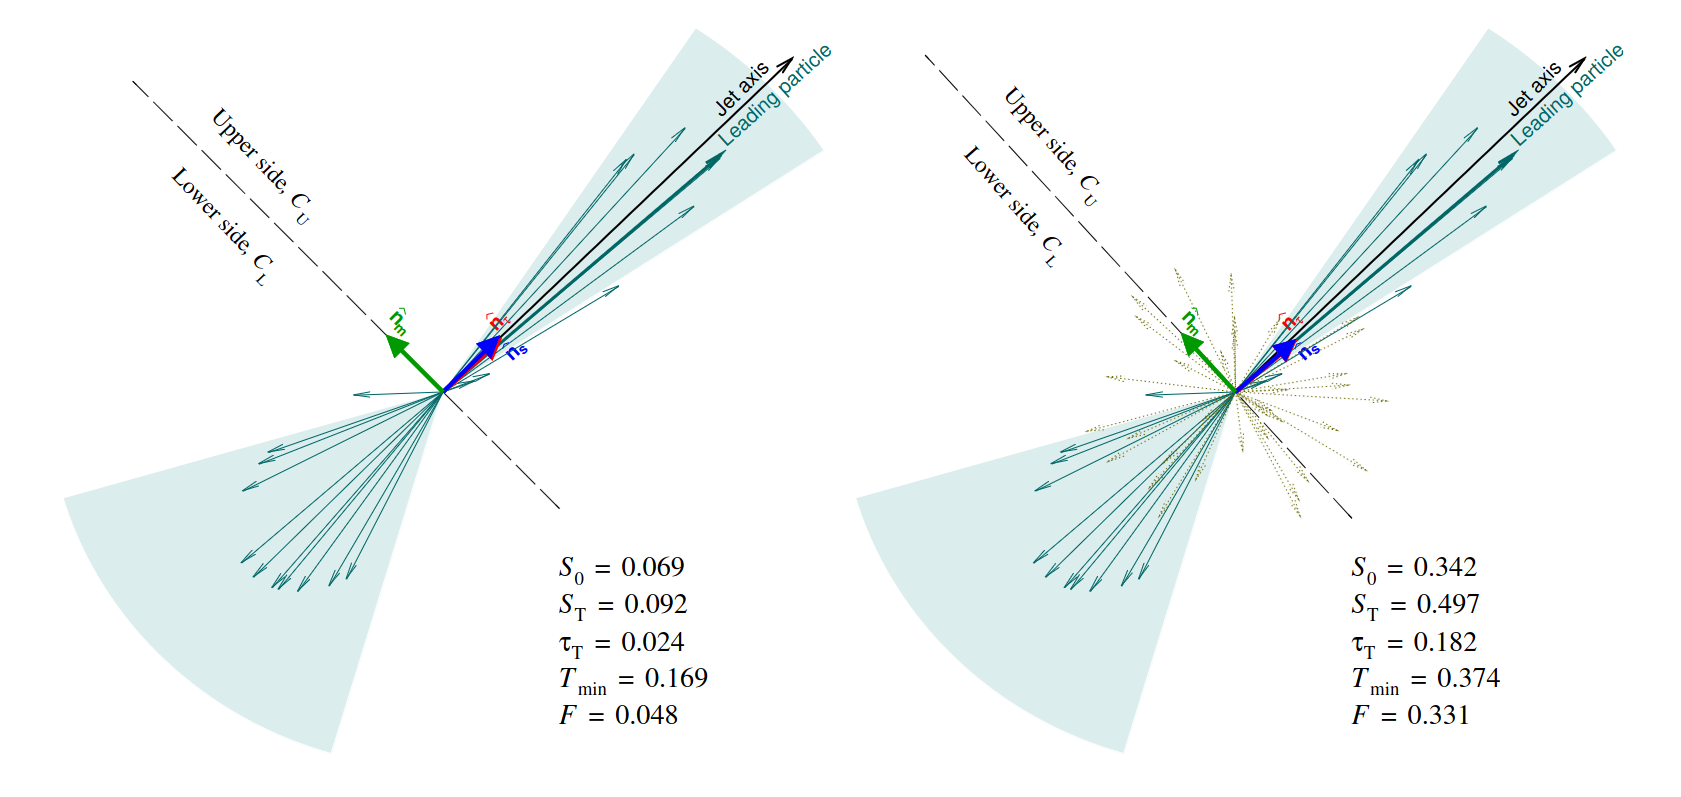
\includegraphics[width=.90\textwidth]{\imgpath/event-observables.png}
\caption{Visualisation of two events in the azimuthal plane: \textbf{(left)} more ``jetty" and \textbf{(right)} more isotropic. Values for the transverse spherocity \SO are given as well as for some other event shape observables: sphericity, thrust, thrust-minor, and F-parameter. The vector minimising the \SO calculation is denoted as a blue arrow. \cite{ortizExperimentalResultsEvent2018}}
\label{fig:sphero:topologies}
\end{figure}

With the discoveries of QGP phenomena in high-multiplicity collisions of small systems, event shape observables become attractive for different reasons. This is because pQCD (``hard") processes are responsible for a significant fraction of particle production and are likely to impact the character of QGP phenomena in non-trivial ways. The role of non-perturbative (``soft") processes is particularly interesting to study as their mechanisms are not fully understood and their interpretation relies on phenomenological models that require clear experimental measurements with high discriminatory power. 

Event shape observables allow us to quantify events according to the dominant contributing processes. For instance, collisions with single large \pt transfer scatterings are likely to lead into events with two back-to-back, highly collimated showers, which create a pencil-like shape in the transverse plane. Conversely, collisions with multiple lower \pt transfer partonic interactions will exhibit a high degree of azimuthal isotropy. Therefore, event shape measurements help us gain a deeper understanding of high-multiplicity events and a better control over the magnitudes of the hard and soft contributions. Ultimately, these measurements may help determine whether QGP formation is necessary in small systems or uncover new physical behaviours.

\subsection{\SO and \SOPT as experimental observables}

Traditionally, spherocity \SO is defined as:

\begin{align}
\SO = \frac{\pi^2}{4} \min_{\hat{n}} \left(\frac{\sum_i
      |p_{\textrm{T},i} \times \hat{n}|}{\sum_i
      |p_{\textrm{T},i}|}  \right)^2 \quad ,
\end{align}
where $p_{\textrm{T},i}$ represents the vector of transverse momentum of a particle $i$ and $\hat{n}$ is the event-dependent unit vector that minimises the sum. The sum runs over all charged particles in the event within the detector acceptance.

Previous ALICE measurements \cite{alicecollaborationChargedparticleProductionFunction2019} studied characteristics of charged particles in pp collisions and discovered their strong dependence of \meanpt on spherocity \SO, which validates the previously discussed motivation. This relationship is shown in Fig.~\ref{fig:sphero:nchpt}. Additionally, phenomenological studies of \SO in Pythia 8 further demonstrate its classifying power by finding strong dependence of \meannmpi as well as the mean number of reconstructed jets $\langle n_\mathrm{j} \rangle$ on \SO\cite{cuautleDisentanglingSoftHard2014, cuautleMidrapidityChargedHadron2015}. These results can be seen in Fig.~\ref{fig:sphero:nmpinjets}.

\begin{figure}%
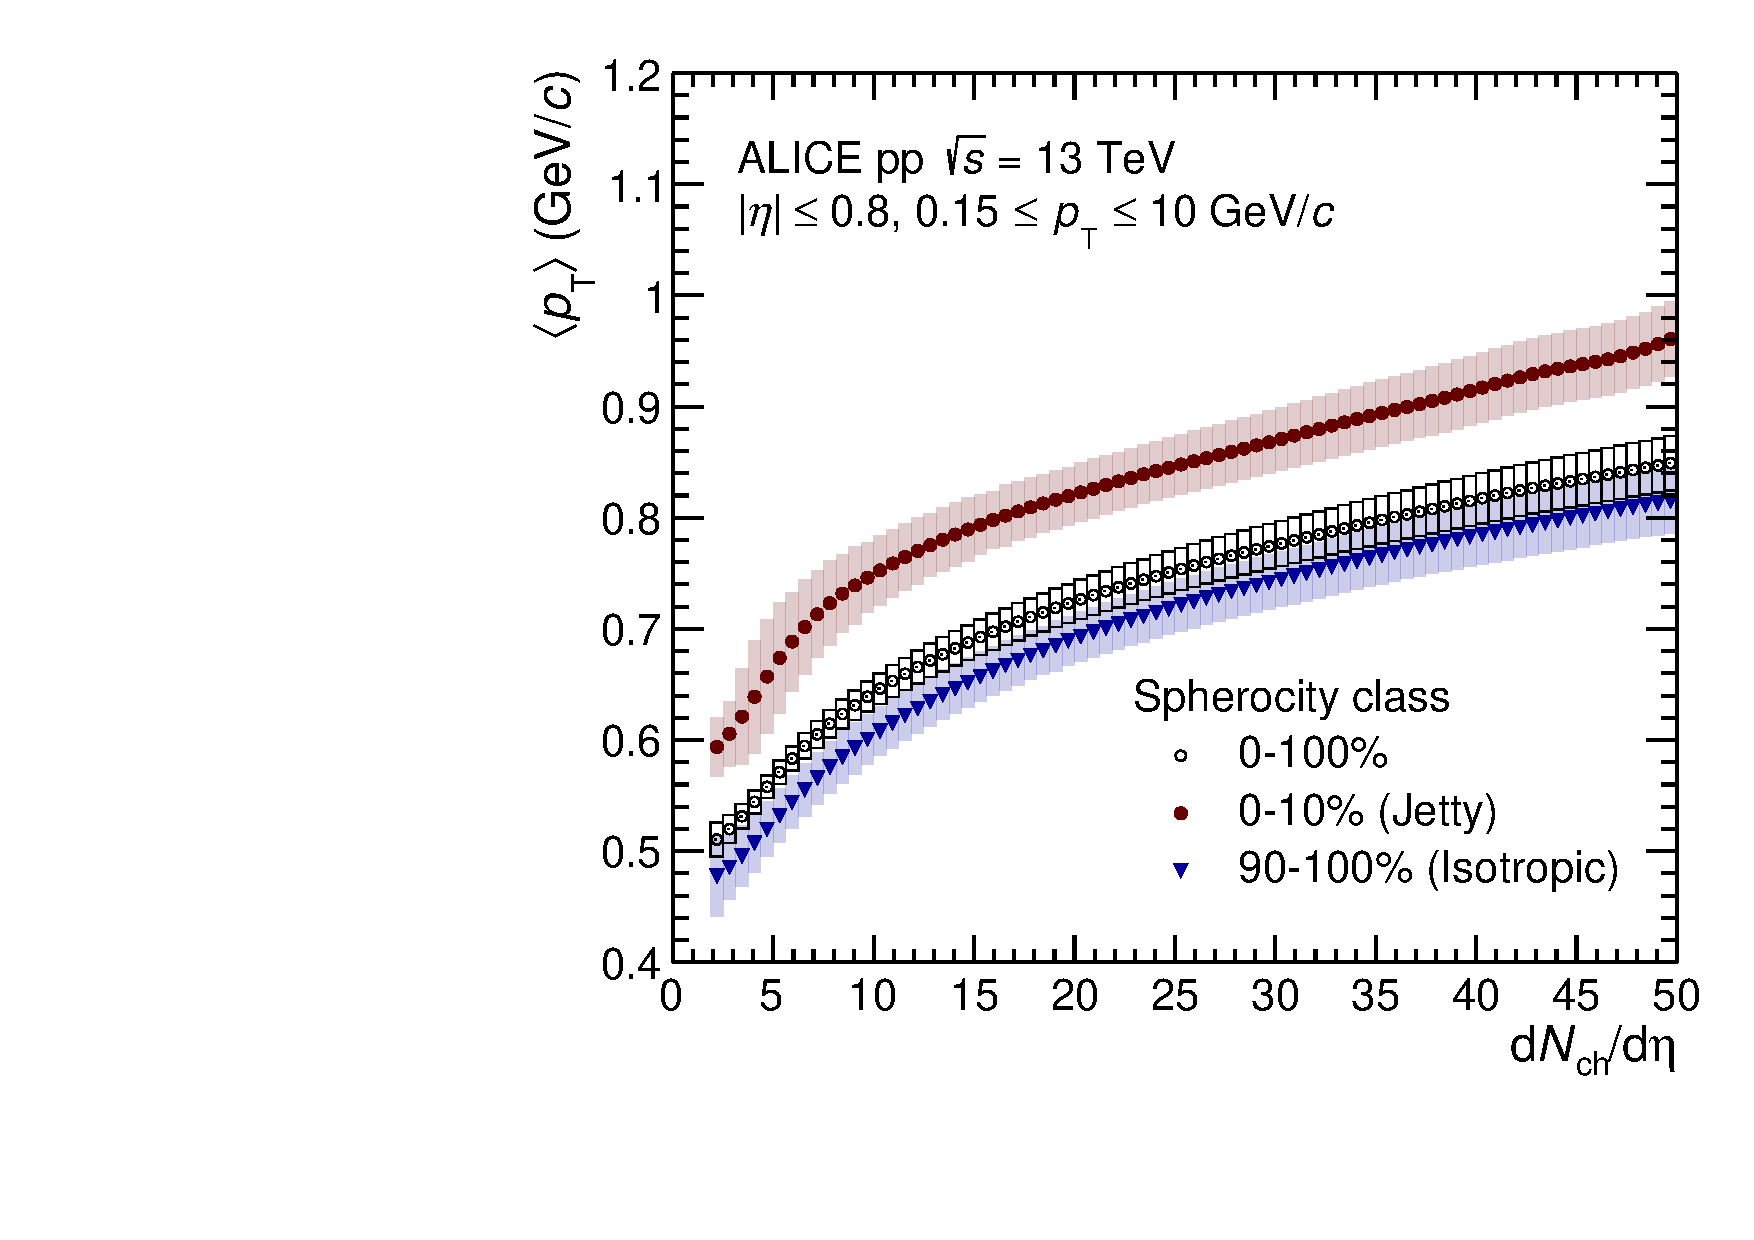
\includegraphics[width=.60\textwidth]{\imgpath/alice_sphero_meanpt.pdf}
\caption{Dependence of the transverse momentum spectrum of charged particles as a function of event multiplicity at mid-rapidity. Cases for jetty, isotropic, and spherocity-unbiased events are displayed. Systematic uncertainties are indicated by the boxes and shaded areas. \cite{alicecollaborationChargedparticleProductionFunction2019}}
\label{fig:sphero:nchpt}
\end{figure}

\begin{figure}%
\subfloat[][]{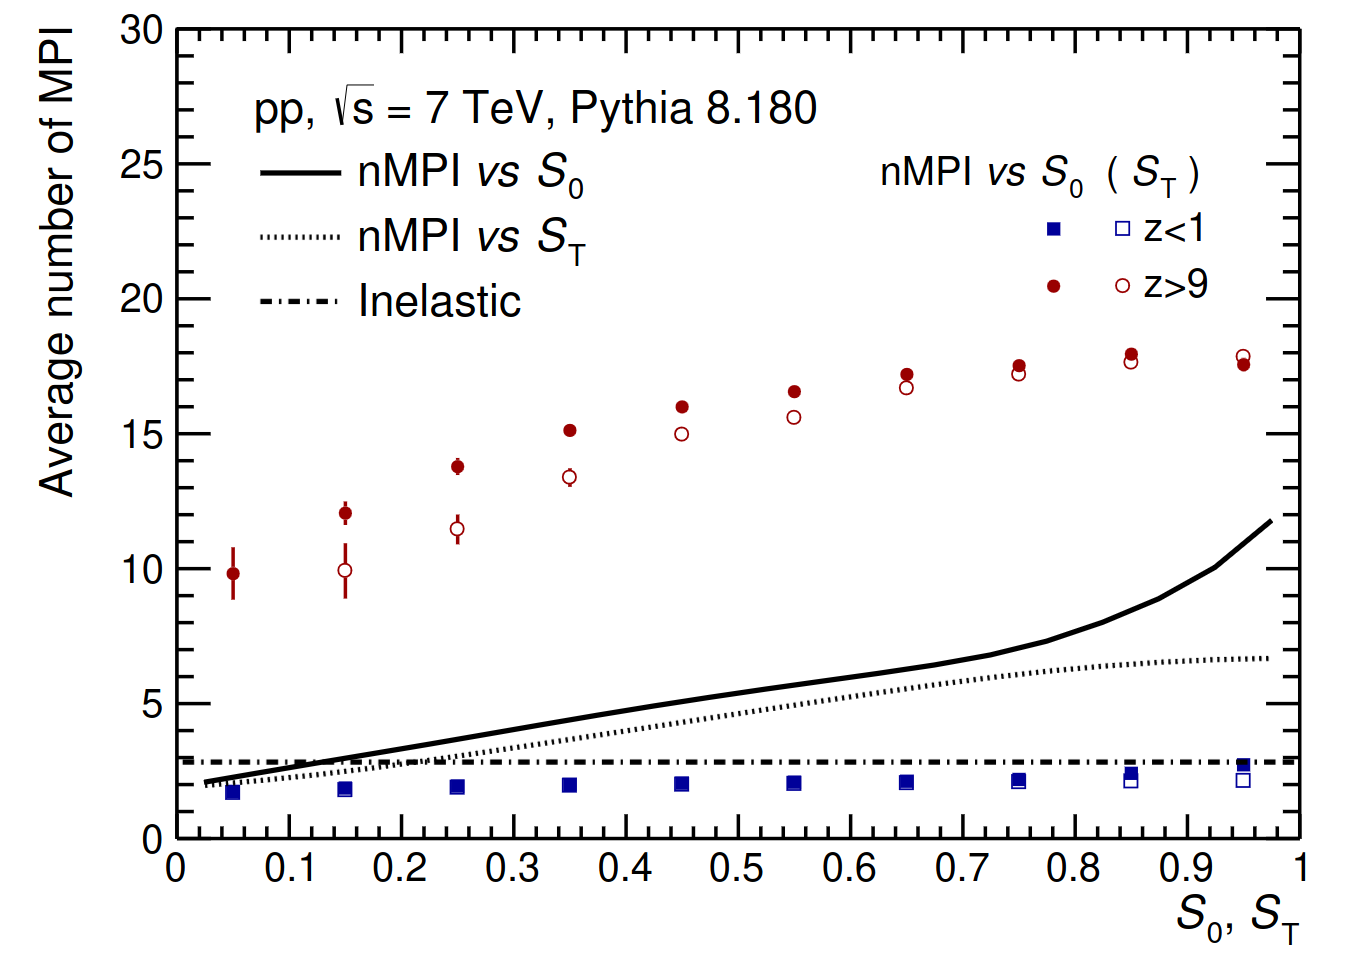
\includegraphics[width=.48\textwidth]{\imgpath/sphero_nmpi.png}}
\subfloat[][]{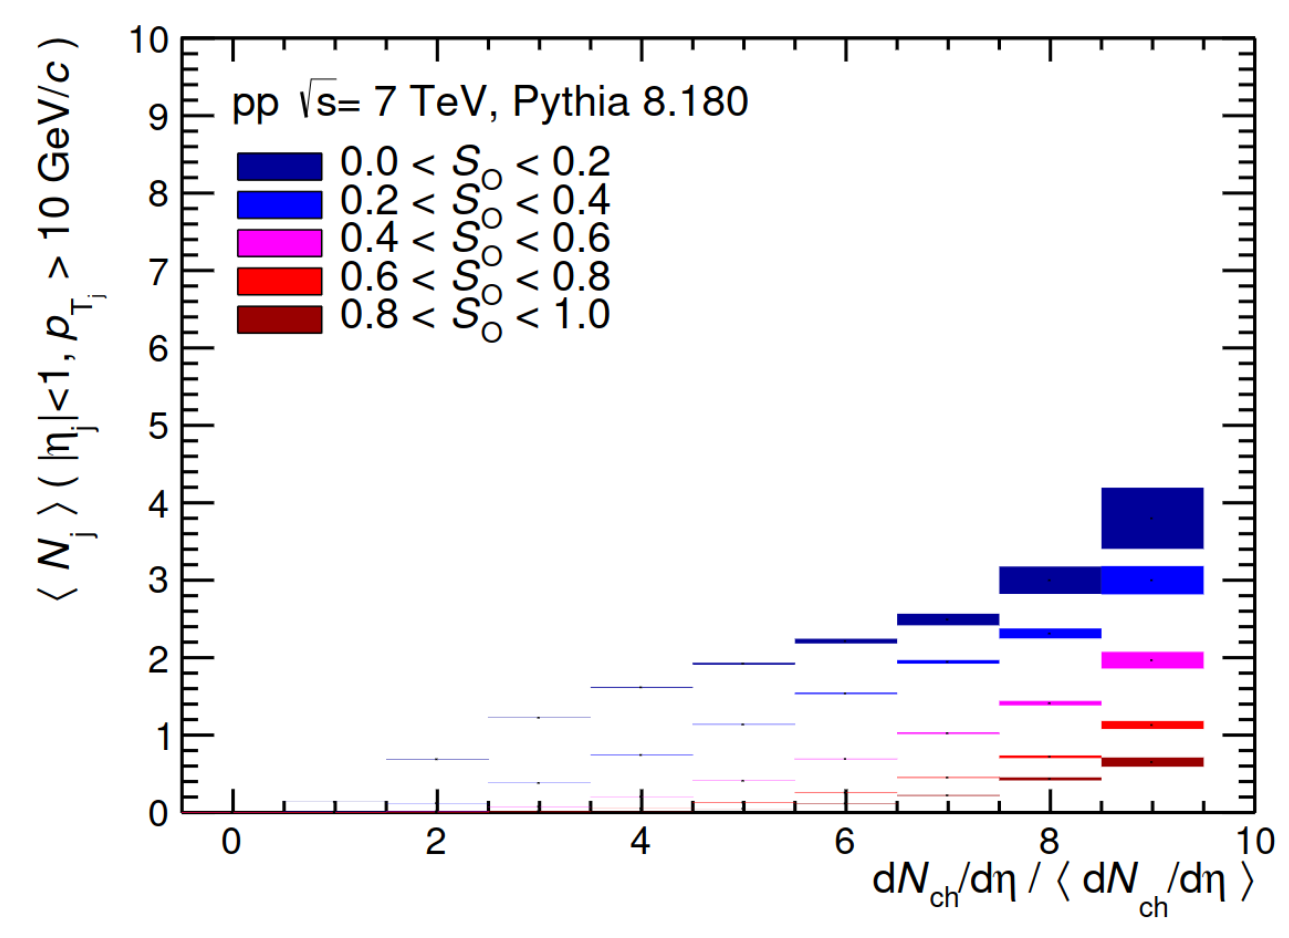
\includegraphics[width=.48\textwidth]{\imgpath/sphero_njets.png}}\\
\caption{\textbf{(a)} Correlation between the mean number of MPIs and transverse spherocity (and sphericity) in pp collisions at \sppt{7} predicted by Pythia 8, shown as solid and dotted lines. The horizontal line shows the average for minimum bias inelastic events. Events with high (red) and low (blue) self-normalised event multiplicity $z$ are also studied and depicted as datapoints. \cite{cuautleDisentanglingSoftHard2014} \textbf{(b)} Average number of reconstructed jets as a function of self-normalised event multiplicity in pp collisions at \sppt{7} with varying values of spherocity, as predicted by Pythia 8. \cite{cuautleMidrapidityChargedHadron2015}}
\label{fig:sphero:nmpinjets}
\end{figure}

This work uses a modified definition of this observable, \textit{unweighted} transverse spherocity \SOPT, defined as follows:

\begin{align}
\SOPT = \frac{\pi^2}{4} \min_{\hat{n}} \left(\frac{\sum_i
      |\hat{p}_{\textrm{T},i} \times \hat{n}|}{N_{\textrm{trks}}}  \right)^2 \quad ,
\label{eq:sOpt}      
\end{align}
where $\hat{p_{\textrm{T},i}}$ represents the \textit{unit} vector of transverse momentum of a particle $i$ and $N_{\textrm{trks}}$ the number of charged particles entering the sum. 

In this thesis, unless stated otherwise, the terms transverse spherocity and spherocity are both used to refer to this unweighted transverse spherocity \SOPT.

Applying the spherocity \SOPT, events in two geometrical limits can be studied:
\begin{itemize}
\item $\SOPT \rightarrow 0$ : the \textbf{``jetty"} limit, where a pencil-like topology is selected. These events are dominated by hard pQCD processes. In this limit, with perfectly collimated back-to-back particles, $\hat{n}$ aligns with them. Thus, the sum of vector products in Eq.~\ref{eq:sOpt} contains only zero values as $\sin 0 = \sin \pi = 0$.
\item $\SOPT \rightarrow 1$ : the \textbf{``isotropic"} limit, where a circular topology is selected. Such events are dominated by multiple softer non-perturbative processes\footnote{However, it is important to mention that  anisotropic collective flow such as $v_2$, a non-perturbative phenomenon, reduces the event isotropy.}. In this limit of $N\rightarrow\infty$ uniformly distributed unit vectors within $(0,2\pi)$, the choice of $\hat{n}$ becomes arbitrary and calculation of the sum in Eq.~\ref{eq:sOpt} leads to:
 \begin{align}
\frac{1}{N} \sum_{n=1}^N | \sin\frac{2\pi n}{N}| &\approx \frac{1}{N} \int_0^N |\sin\frac{2\pi x}{N}| \mathrm{d}x \\ 
&= \frac{2}{N} \int_0^{N/2} \sin\frac{2\pi x}{N} \mathrm{d}x = \frac{1}{\pi} \int_0^{\pi} \sin u \mathrm{d}u \\
&= \frac{1}{\pi} \left[-\cos x\right]_0^{\pi} = \frac{2}{\pi} \quad \,
\end{align}
and therefore $\SOPT=1$. 
\end{itemize}

Figure~\ref{fig:sphero:shapelimits} illustrates how spherocity slowly approaches the circular limit value with increasing $N$ compared to other event shape observables. This property makes spherocity favoured by experimentalists in these measurements, as it provides the highest discrimination power of isotropic events \cite{ortizExperimentalResultsEvent2018}.

\begin{figure}%
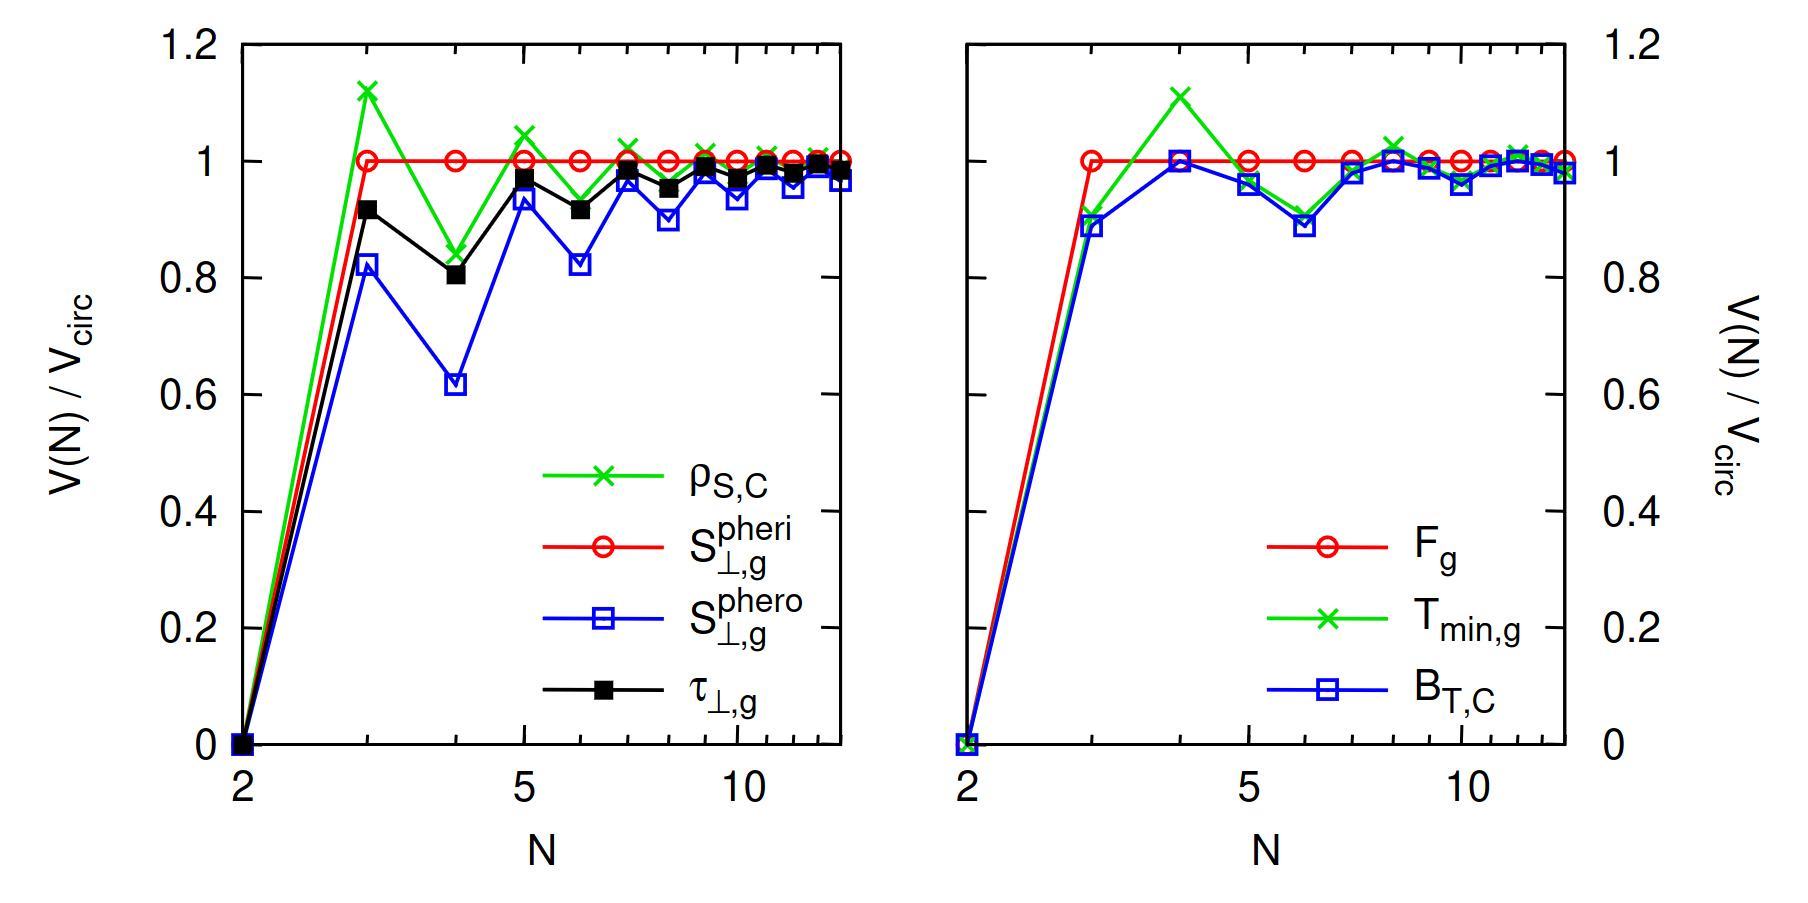
\includegraphics[width=.90\textwidth]{\imgpath/sphero-shapelimits.png}
\caption{Graphs showing how rapidly the different event shape observables approach the circular limit $V_\mathrm{circ}$ corresponding to $N\to\infty$, based on the number of perfectly isotropically distributed particles $N$. Transverse spherocity, here denoted as $S^\mathrm{phero}_{\perp,g}$, exhibits the slowest rise, and never exceeds unity.\cite{banfiPhenomenologyEventShapes2010}}
\label{fig:sphero:shapelimits}
\end{figure}


\subsection{Relationship between \SOPT and \SO}

In ALICE, only charged particles are considered when calculating spherocities. This introduces biases when measuring charged and neutral species of hadrons. For instance, even topologically identical events with dominant high-\pt leading $\pi^+$ and $\pi^0$ can yield significantly different values of the traditional \pt-weighted spherocity \SO, despite being comparable in all relevant aspects. In contrast, unweighted spherocity \SOPT offers a more similar quantification of the two events, as shown in Fig.~\ref{fig:sphero:sOvssOpt}. However, it should be noted that this modified definition is only applicable to events with many tracks (i.e., $N_{\textrm{trks}}>10$).

\begin{figure}%
\includegraphics[width=.70\textwidth]{\imgpath/SOvsSOPT2_up.png}
\caption{Illustration of two topologically identical events with swapped charged and neutral particles. Momentum vectors entering the \pt-weighted spherocity (red) and \pt-unweighted (blue) calculations are displaying, showing a larger difference between the two scenarios for the former than the latter. (\textit{Needs to be remade or credited})}
\label{fig:sphero:sOvssOpt}
\end{figure}

In addition, while not a large concern in high-multiplicity collisions \cite{alicecollaborationChargedparticleProductionFunction2019}, \SOPT also offers improved resolution compared to \SO, as the failure to reconstruct a high-\pt track has a smaller impact. Overall, \SO and \SOPT exhibit similar values and interpretations, with a strong correlation between the two, as illustrated in Fig.~\ref{fig:sphero:sOvssOptcorr}.

\begin{figure}%
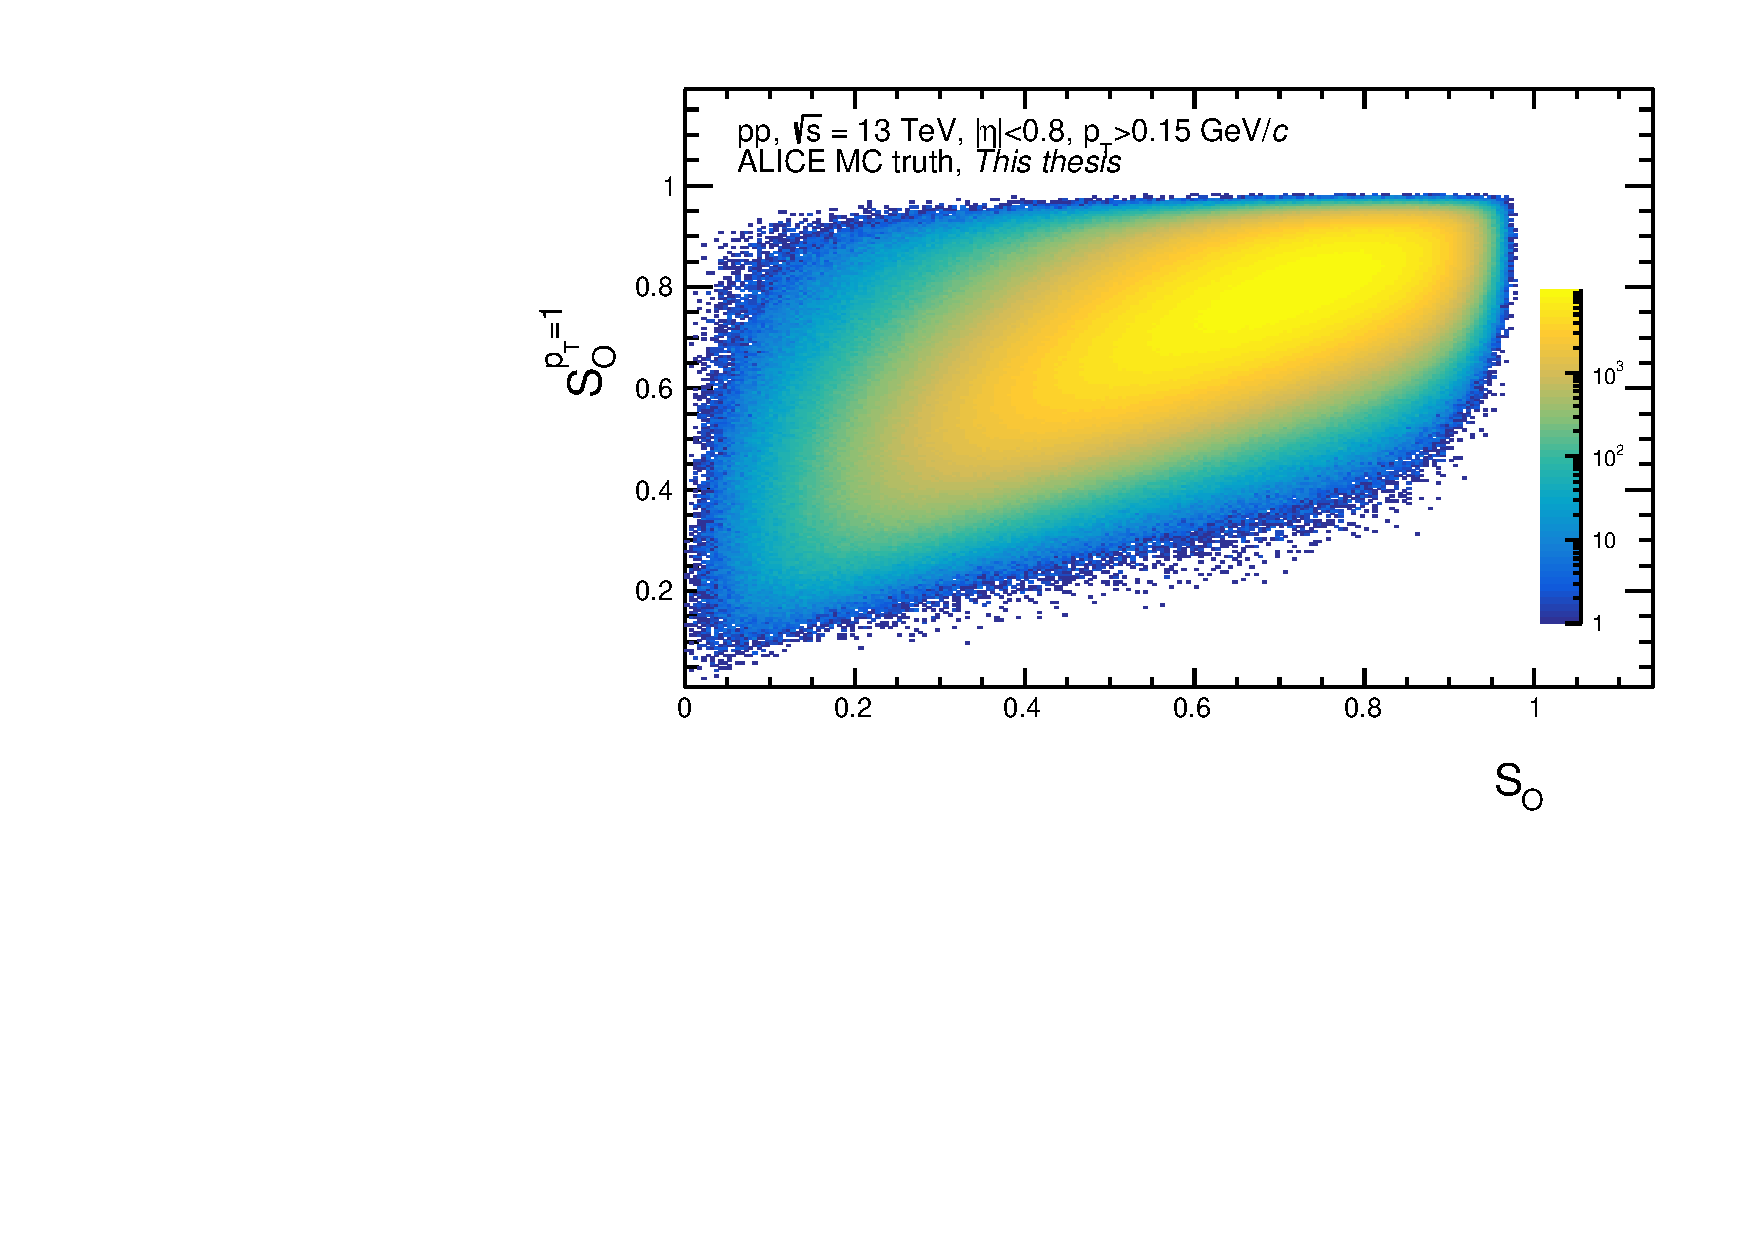
\includegraphics[width=.70\textwidth]{\imgpath/InfoSO_norm.pdf}
\caption{Two-dimensional histogram showing the correlation between the traditional transverse spherocity \SO and the unweighted transverse spherocity \SOPT employed in this measurement, obtained from ALICE MC simulations.}
\label{fig:sphero:sOvssOptcorr}
\end{figure}

\subsection{Track and event selection}\label{sec:sphero:eventtracks}

The measurements are carried out on MB events with \INELgtO, requiring at least one hit in the \VOA or \VOC scintillators and one charged particle reconstructed within $|\eta|<1$. The primary vertex is reconstructed using hits in the SPD and is required to be within $10$~cm of the interaction point. The fast read-out time of the SPD allows rejection of out-of-bunch pile-up. In-bunch pile-up is further removed by excluding events with multiple reconstructed vertices. The presented results are based on high-multiplicity events, selected by the classifiers \VOM (forward rapidity) and \tracklet (mid-rapidity), and require a minimum of 10 reconstructed tracks within $|\eta|<0.8$ and with $\pt>\gevc{0.15}$.

To ensure a high level of azimuthal acceptance uniformity, which is important for event shape measurements, the following, rather loose, selection criteria are employed:
\begin{enumerate}
\item The SPD is not used due to its inactive sectors, at the expense of a lower momentum resolution.
\item A track is required to have at least 50 clusters in the TPC and be matched to hits in the ITS to improve tracking precision and further reject  pile-up.
\item DCA cuts are applied in both the longitudinal ($|\mathrm{DCA}_z|<3.2$~cm) and transverse ($|\mathrm{DCA}_{xy}|<2.4$~cm) planes to ensure that the reconstructed TPC track points to the primary vertex.
\end{enumerate}
It should be noted that charged decay products of \VOs with low \pt ($\lesssim \gevc{1}$) and small decay radius may enter and influence \SOPT determination.

\subsection{Multiplicity selection and its interplay with \SOPT}

Spherocity exhibits a twofold correlation with multiplicity that is not particularly informative. First, the definition of \SOPT results in higher values for events with more uniformly distributed particles, as shown in Fig.~\ref{fig:sphero:shapelimits}. Second, in models such as Pythia, high multiplicity is often associated with more MPI, which tend to lead to higher isotropy due to the increased number of emission sources. To gain a more nuanced understanding of the relationship between spherocity and multiplicity, the effect of \SOPT on measured particles was analysed in high-multiplicity events determined in two distinct rapidity regions, as described above. Specifically, the top $1\%$ ($10\%$) quantiles are used, denoted as \VOM I and \NSPD I (\VOM I-III and \NSPD I-III).

Figure~\ref{fig:sphero:v0mvscl1} shows the effect of \SOPT on the pion yields and \meanpt. Pions are measured in the high-multiplicity events and in top and bottom $10\%$ and $1\%$ quantiles of \SOPT. The result reveals that when measuring multiplicity in forward rapidity (\VOM I), the effect of \SOPT causes a change of approximately $100\%$ in the yields when going from jetty to isotropic limits, whereas the difference in \meanpt is only about $10\%$. Conversely, when determining the multiplicity in mid-rapidity (\NSPD I), the same region where the pion spectra are reconstructed, the change in the yields is only approximately $10\%$ while the change in \meanpt is approx.\ $25\%$.

For this reason, the following combinations of multiplicity and \SOPT selections are presented:
\begin{enumerate}
\item \NSPD I and \SOPT top and bottom $10\%$ quantiles: This selection emphasises the impact of extreme event topologies on the QCD processes whilst minimising the effect of multiplicity dependence.
\item \NSPD I-III and \SOPT top and bottom $1\%$ quantiles: This selection shows the effect of even more extreme event topologies but with overall less and somewhat varying multiplicity. 
\item \VOM I and \SOPT top and bottom $10\%$ quantiles: This selection highlights the effect of extreme event topologies with highly varying mid-rapidity multiplicity. It also allows for a comparison with \NSPD I-III and \SOPT $1\%$ selection, as the mid-rapidity multiplicity and the \meanpt variations are more similar.
\end{enumerate}

\begin{figure}%
\begin{tikzpicture}
    \draw (0, 0) node[inner sep=0] {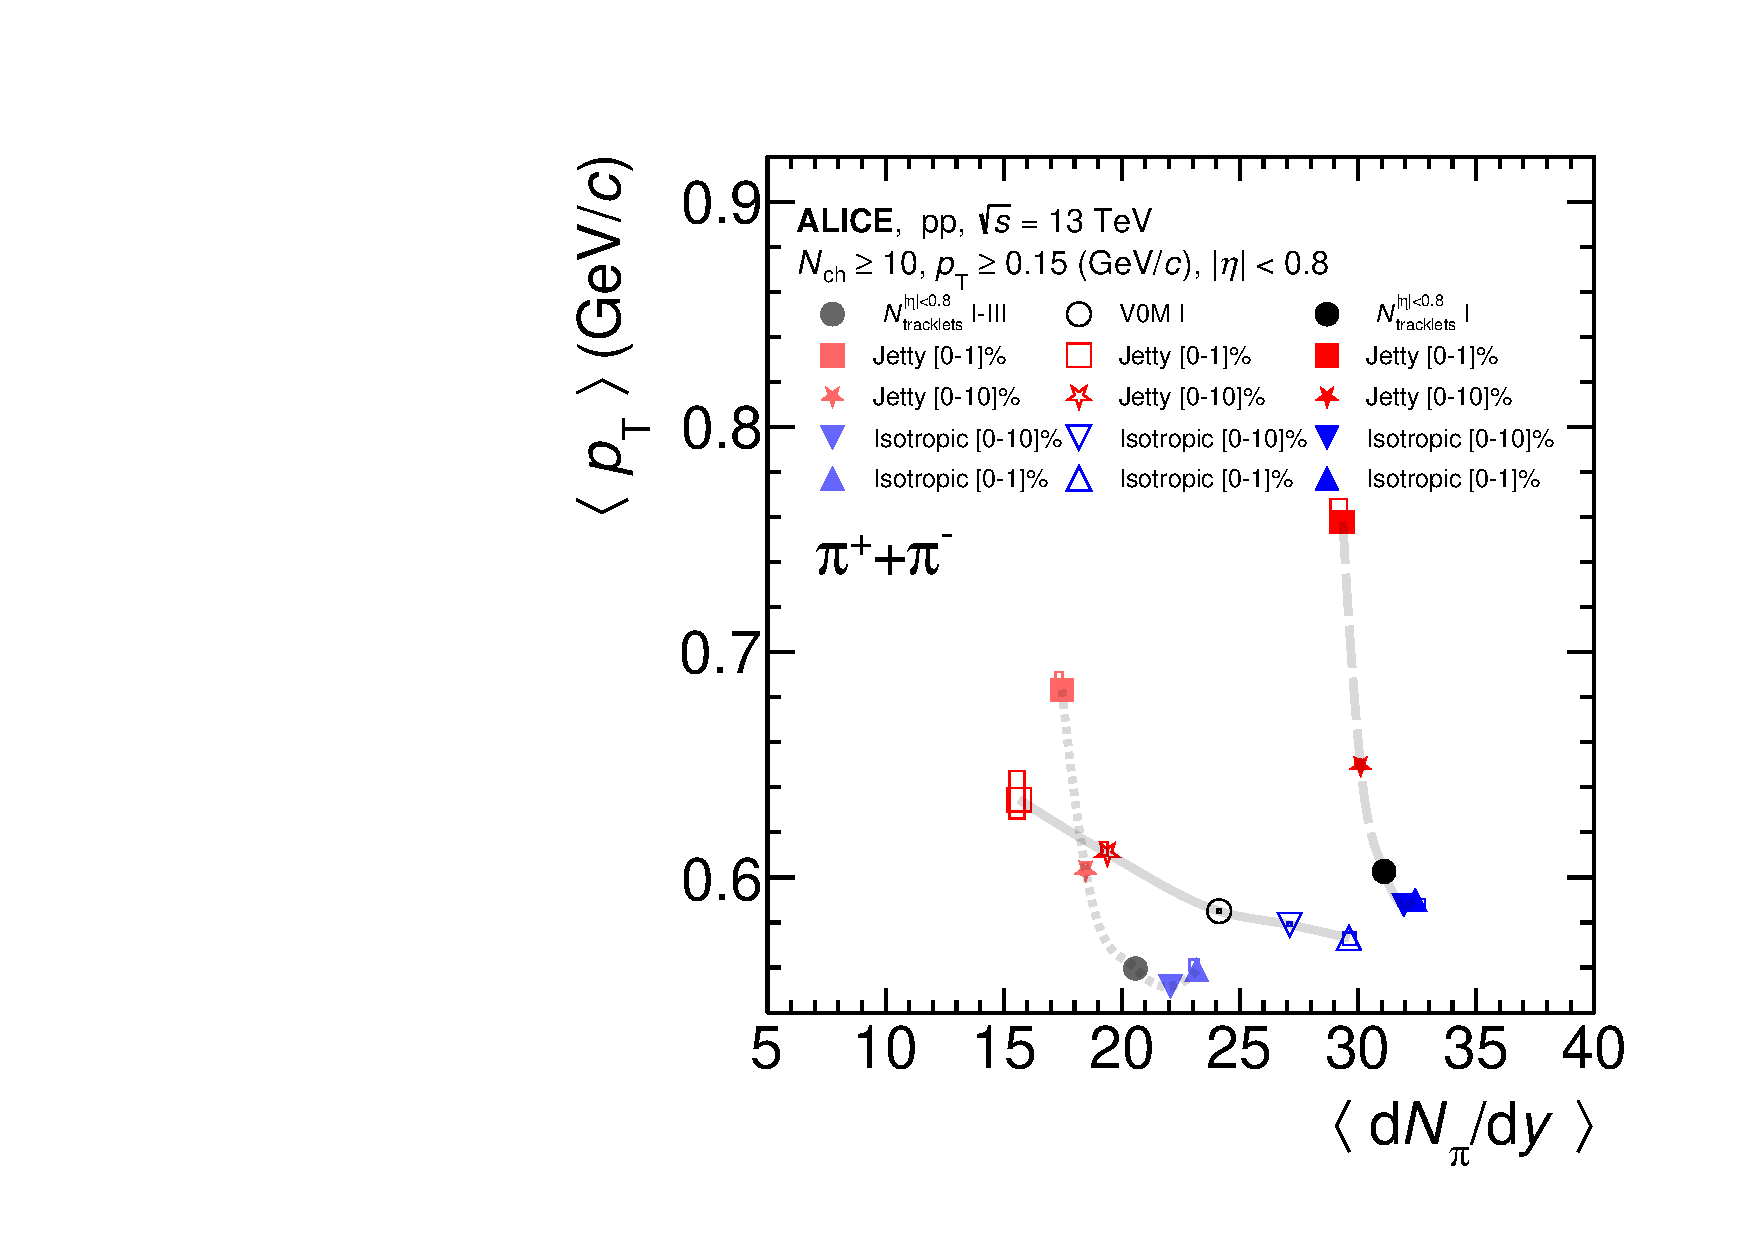
\includegraphics[width=.70\textwidth]{\imgpath/mgPion_0.pdf}};
    \draw (-1.5, -0.2) node {This thesis};
\end{tikzpicture}
\caption{Relationship between the mean transverse momentum of charged pions and their yields in events with different \SOPT values and event multiplicity determined at mid-rapidity (here denoted $N_\mathrm{tracklets}^{|\eta|<0.8}$) and forward rapidity (VOM). Events in the same multiplicity classes are connected with lines for clarity's sake.}
\label{fig:sphero:v0mvscl1}
\end{figure}

The mid-rapidity multiplicities in the different high-multiplicity classes are reported in Tab.~\ref{tab:sphero:hm}. The measured \SOPT distributions in \NSPD I, \NSPD I-III, and \VOM I-III are shown in Fig.~\ref{fig:sphero:sopt}. They are treated with Bayesian unfolding to account for reconstruction effects. They are also compared with theoretical predictions from Pythia 8 (Monash \cite{skandsTuningPYTHIAMonash2014} and Ropes \cite{bierlichEffectsOverlappingStrings2015} tunes), EPOS LHC \cite{pierogEPOSLHCTest2015}, and Herwig 7 \cite{bellmHerwigReleaseNote2020}. Table~\ref{tab:sphero:sOpt} provides the \SOPT cut values associated with the quantile selections in data.

\begin{figure}[H]%
\subfloat[][]{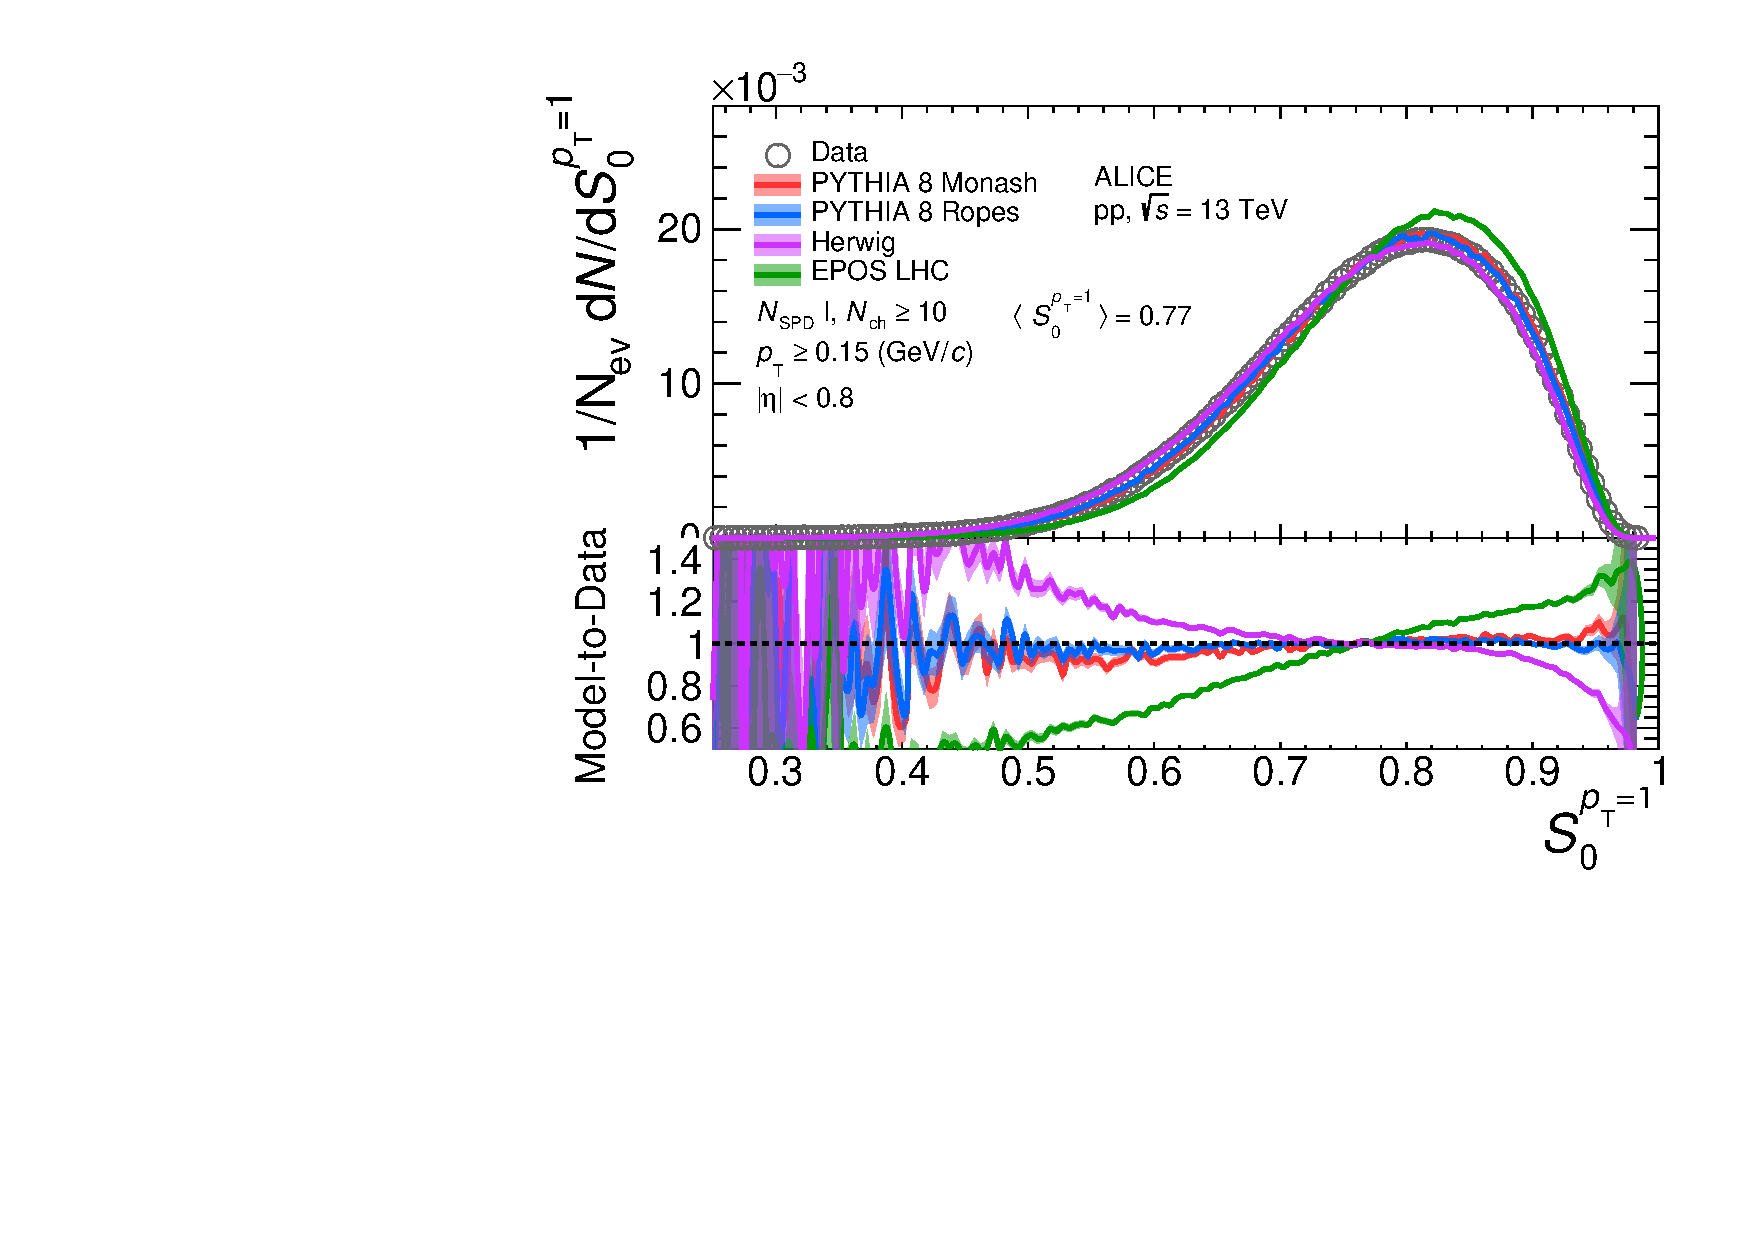
\includegraphics[width=.45\textwidth]{\imgpath/SO_Unfolded_CL1_Perc_1.pdf}}
\subfloat[][]{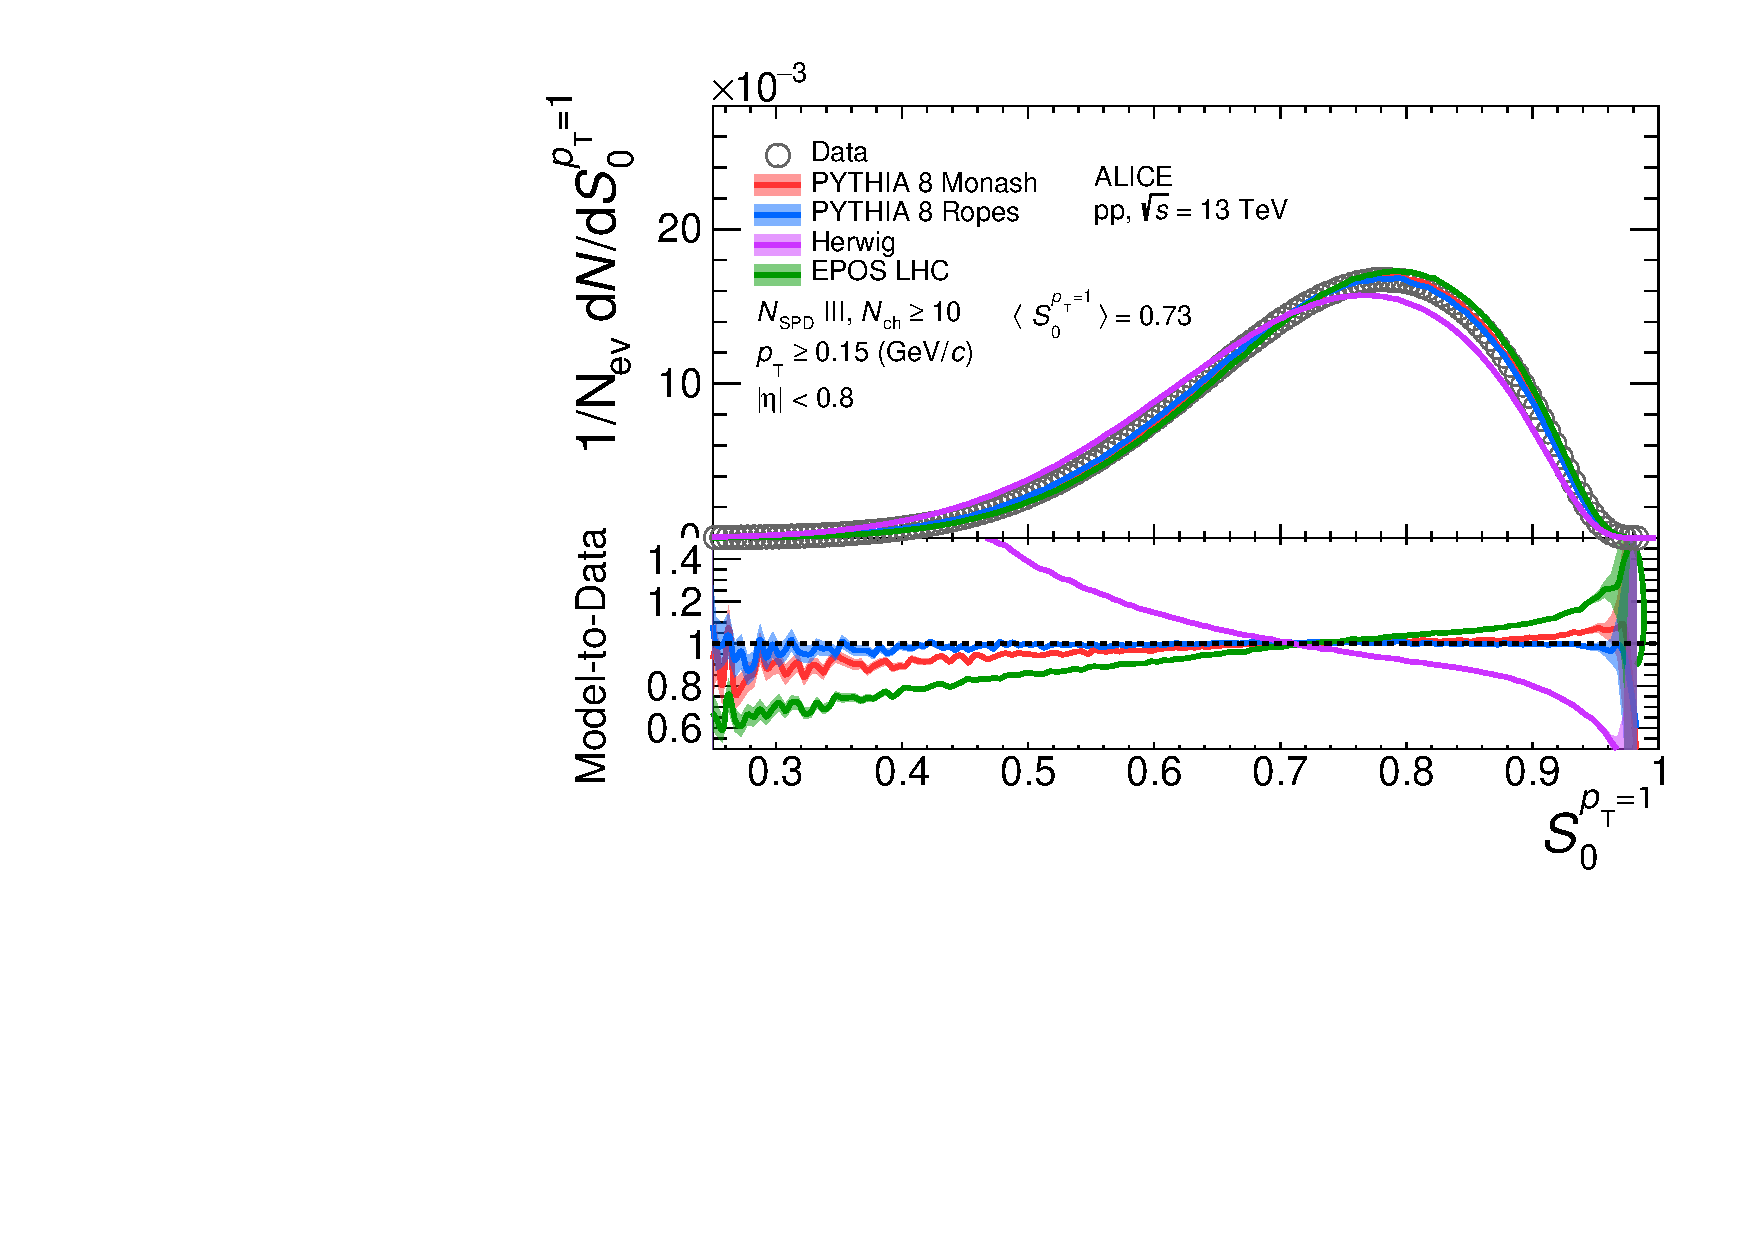
\includegraphics[width=.45\textwidth]{\imgpath/SO_Unfolded_CL1_Perc_10.pdf}}\\
\subfloat[][]{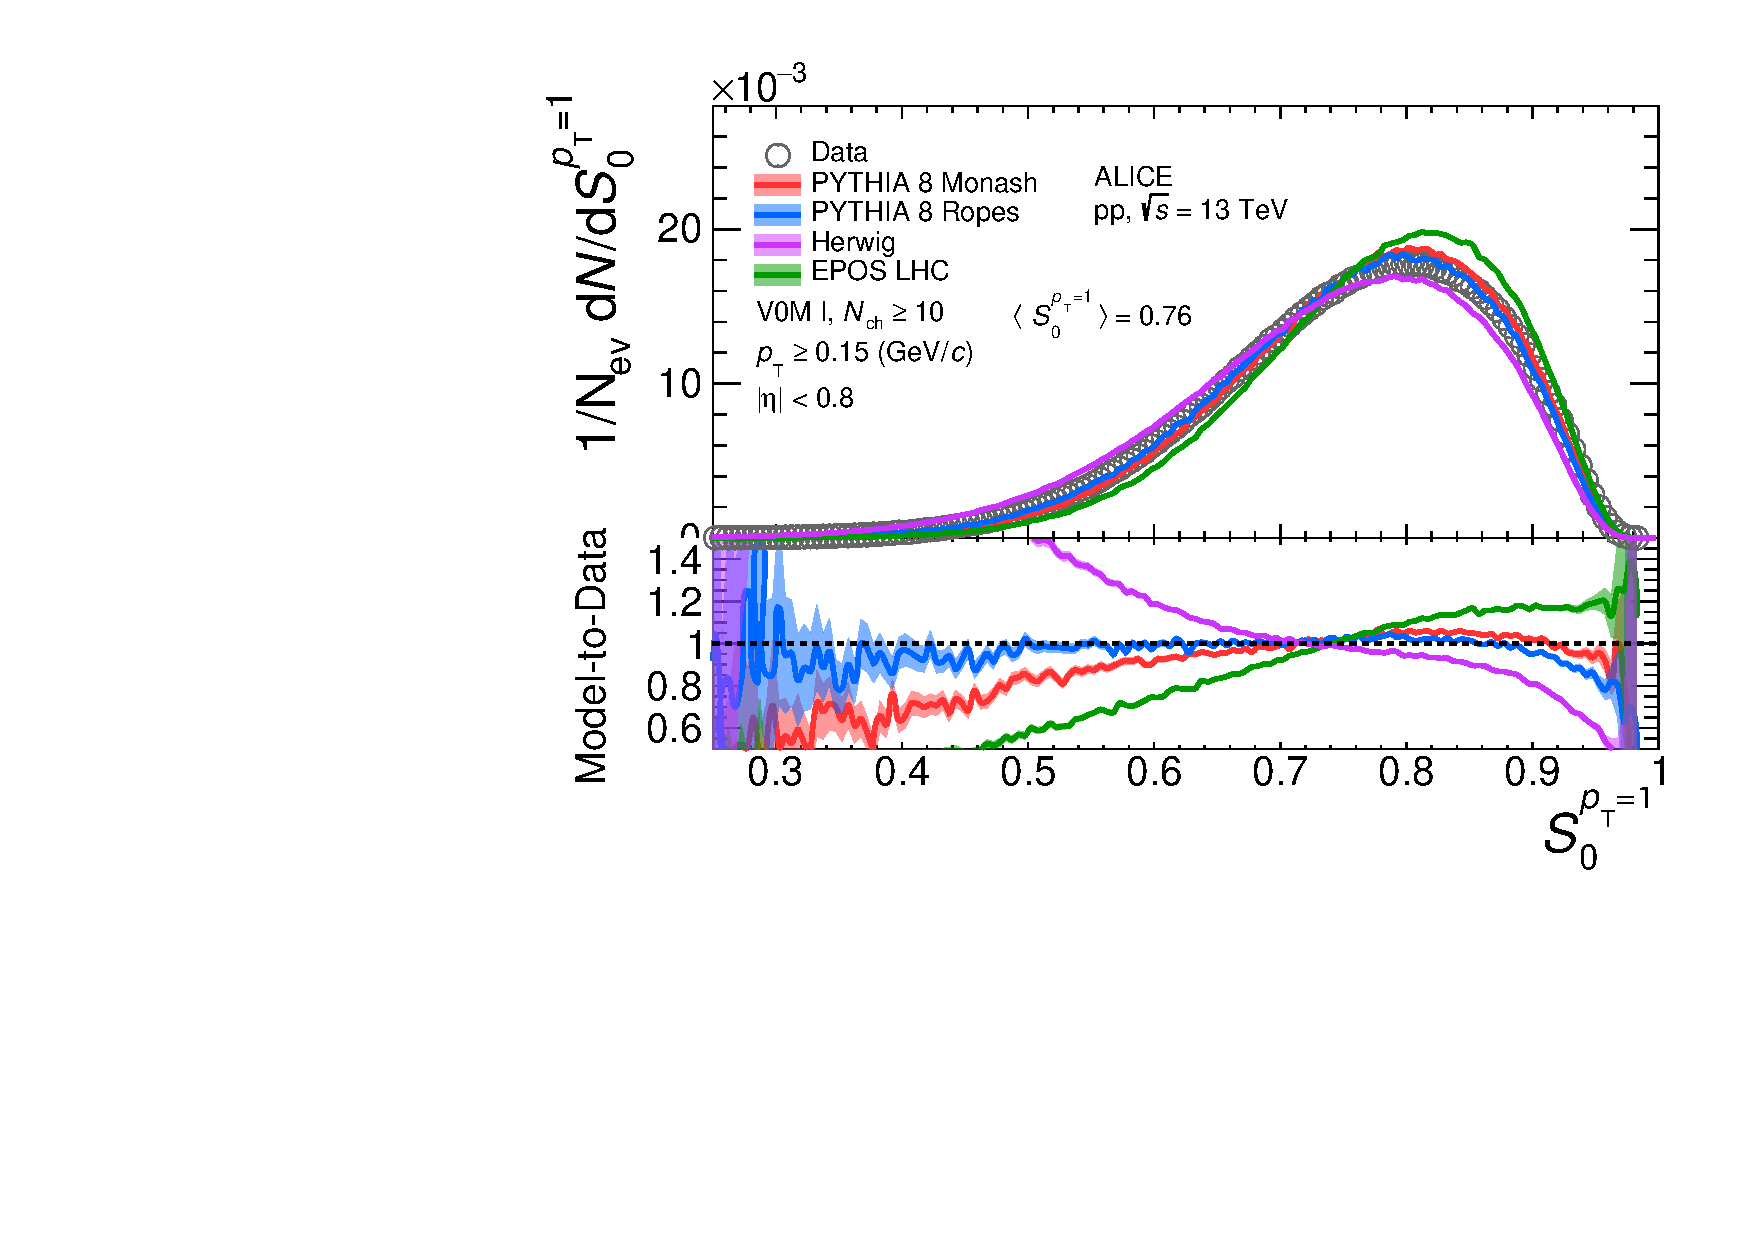
\includegraphics[width=.45\textwidth]{\imgpath/SO_Unfolded_V0M_Perc_1.pdf}}
\caption{The measured and fully corrected \SOPT distributions for both \textbf{(a)} \NSPD 0--1\%, \textbf{(b)} 0--10\% and \textbf{(c)} \VOM 0--1\% . The curves represent different model prediction, where the shaded area represents the statistical uncertainty of the models.}
\label{fig:sphero:sopt}
\end{figure}

%ˇ\begin{table}[h]
%\centering
%\caption{TBA}
%\label{tab:sphero:hm}
%\begin{tabular}{|c|c|c|c|c|}
%\hline
%\textbf{Event class} & \textbf{\NSPD I} & \textbf{\NSPD I-III} & %\textbf{\VOM I} & \textbf{\VOM I-III} \ \hline
%$\avdndeta$ & $18.7 \pm 0.25$ & $21.57 \pm 0.32$ & $26.02 \pm 0.35$ & %$33.01 \pm 0.55$ \ \hline
%\end{tabular}
%\end{table}

\begin{table}[h!]
\centering
\caption{Mean values of charged particle multiplicity at mid-rapidity in different high-multiplicity event classes.}
\label{tab:sphero:hm}

\begin{tabular}{|cc|ccc|}
\hline
\multicolumn{2}{|r|}{\parbox[b][1.2em]{2em}{} Event class} & \NSPD I & \NSPD I-III & \VOM I \\ \hline
%\multicolumn{2}{l|}{} & \multicolumn{3}{l}{} \\
%\multicolumn{5}{l}{\parbox[b][1.4em]{1em}{Jetty}} \\ \hline
\multicolumn{2}{|l|}{\parbox[b][1.1em]{1em}{}\avdndeta} & $33.01 \pm 0.55$ & $21.57\pm 0.32$ & $26.02 \pm 0.35$ \\ \hline
\end{tabular}
\end{table}

\begin{table}[h!]
\centering
\caption{Cut values of the different quantiles of the uncorrected \SOPT distribution used for the event selections in this analysis.}\label{tab:sphero:sOpt}

\begin{tabular}{|cc|ccc|}
\hline
\multicolumn{2}{|r|}{\parbox[b][1.2em]{2em}{} Event class} & \NSPD I & \NSPD I-III & \VOM I \\ \hline
%\multicolumn{2}{l|}{} & \multicolumn{3}{l}{} \\
\multicolumn{5}{l}{\parbox[b][1.4em]{1em}{Jetty}} \\ \hline
\multicolumn{2}{|l|}{\parbox[b][1.1em]{1em}{}\SOPT 0--1\%} & $<0.487$ & $<0.408$ & $<0.433$ \\
\multicolumn{2}{|l|}{\SOPT 0--10\%} & $<0.624$ & $<0.561$ & $<0.589$ \\
\hline
\multicolumn{5}{l}{\parbox[b][1.2em]{1em}{Isotropic}} \\ \hline
\multicolumn{2}{|l|}{\SOPT 90--100\%} & $>0.892$ & $>0.871$ & $>0.882$ \\
\multicolumn{2}{|l|}{\SOPT 99--100\%} & $>0.942$ & $>0.930$ & $>0.936$ \\ \hline
\end{tabular}
\end{table}

\subsection{Comparison of \VO production with MC generators}

Further on in this chapter, the results of \KOs, \LA, and \AL as a function of \SOPT are presented and compared with predictions from phenomenological models Pythia 8 \cite{bierlichComprehensiveGuidePhysics2022}, EPOS LHC \cite{pierogEPOSLHCTest2015}, and Herwig 7 \cite{bellmHerwigReleaseNote2020} obtained from MC simulations. To mitigate the effect of reconstruction on the experimental results and make the comparison with these predictions as comparable as possible, the following strategies were employed based on findings using the ALICE MC simulations:
\begin{itemize}
\item The results were compared using the same quantiles of the \SOPT distributions in both the MC and the data, instead of relying on the experimental \SOPT ranges determined by specific cut values. This approach reduced the effects of \SOPT resolution.
\item In the MC simulations, the \SOPT calculations included neutral particles \KOs, \LA, and \AL, despite their neutral charge. This helped minimize differences between the true and reconstructed/corrected MC results, possible due to the potential contribution of charged daughters to the \SOPT calculation. 
\end{itemize}
Any discrepancies that still persisted between the true and reconstructed/corrected transverse momentum spectra were accounted for as systematic uncertainties.

\section{Systematic uncertainties}

The systematic uncertainties associated with the \pt spectra of \KOs, \LA, and \AL were evaluated separately for \NSPD I and \VOM I events with no \SOPT selection, as well as for the top and bottom $10\%$ isotropic and jetty quantiles, using the methodology described in Section~\ref{sec:ana:syst}. The relative systematic uncertainties obtained from these configurations were also applied to the \NSPD I-III and \VOM I-III event classes with different jetty/isotropic quantiles.

Figures~\ref{fig:sphero:systK0s}, \ref{fig:sphero:systLA}, and \ref{fig:sphero:systAL} illustrate the maximal deviations of variations resulting from alternative cut values, extraction parameters, or feeddown methods in \VOM I, \SOPT-unbiased events for \KOs, \LA, and \AL, respectively. 

\begin{figure}[H]
  \centering
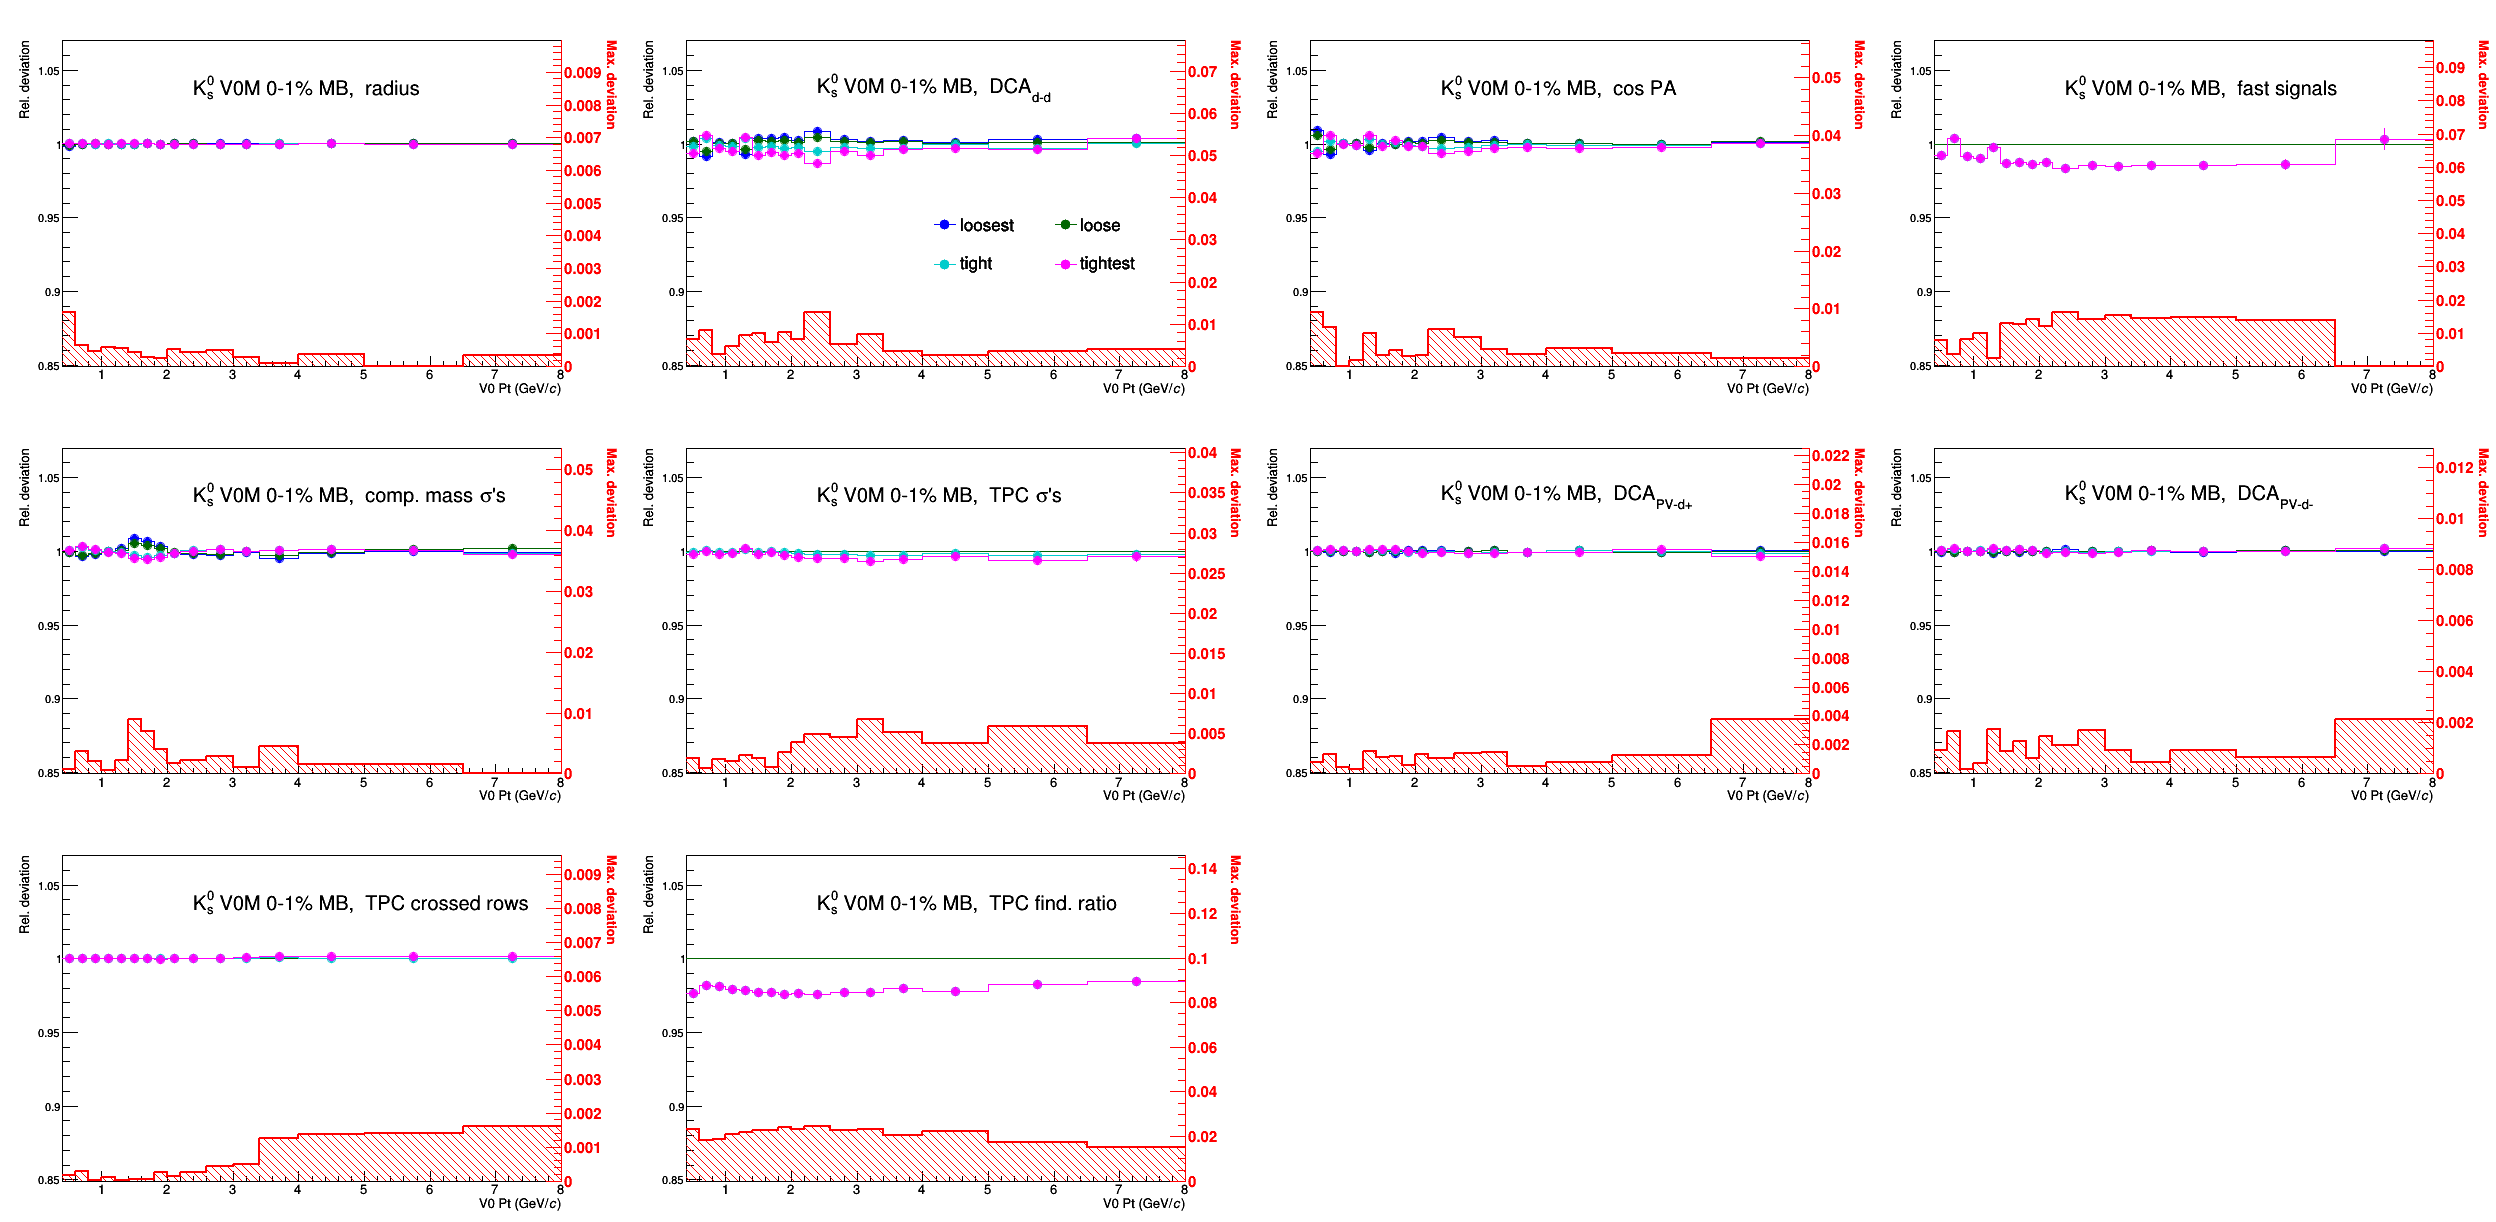
\includegraphics[width=.98\textwidth]{\imgpath/cDev_K0s_V0M01_MB.png}
  \caption{NEEDS TO BE REDRAWN IN CONSISTENT STYLE WITH RT CHAPTER:Deviations of the corrected spectra w.r.t.\ the different cut variations used for the \Ks . The maximum deviation is added in quadrature to the total, if it's larger than $\sigma_\mathrm{RB}$ (depicted as errorbars) from unity.}
  \label{fig:sphero:systK0s}
\end{figure}

\begin{figure}[H]
  \centering
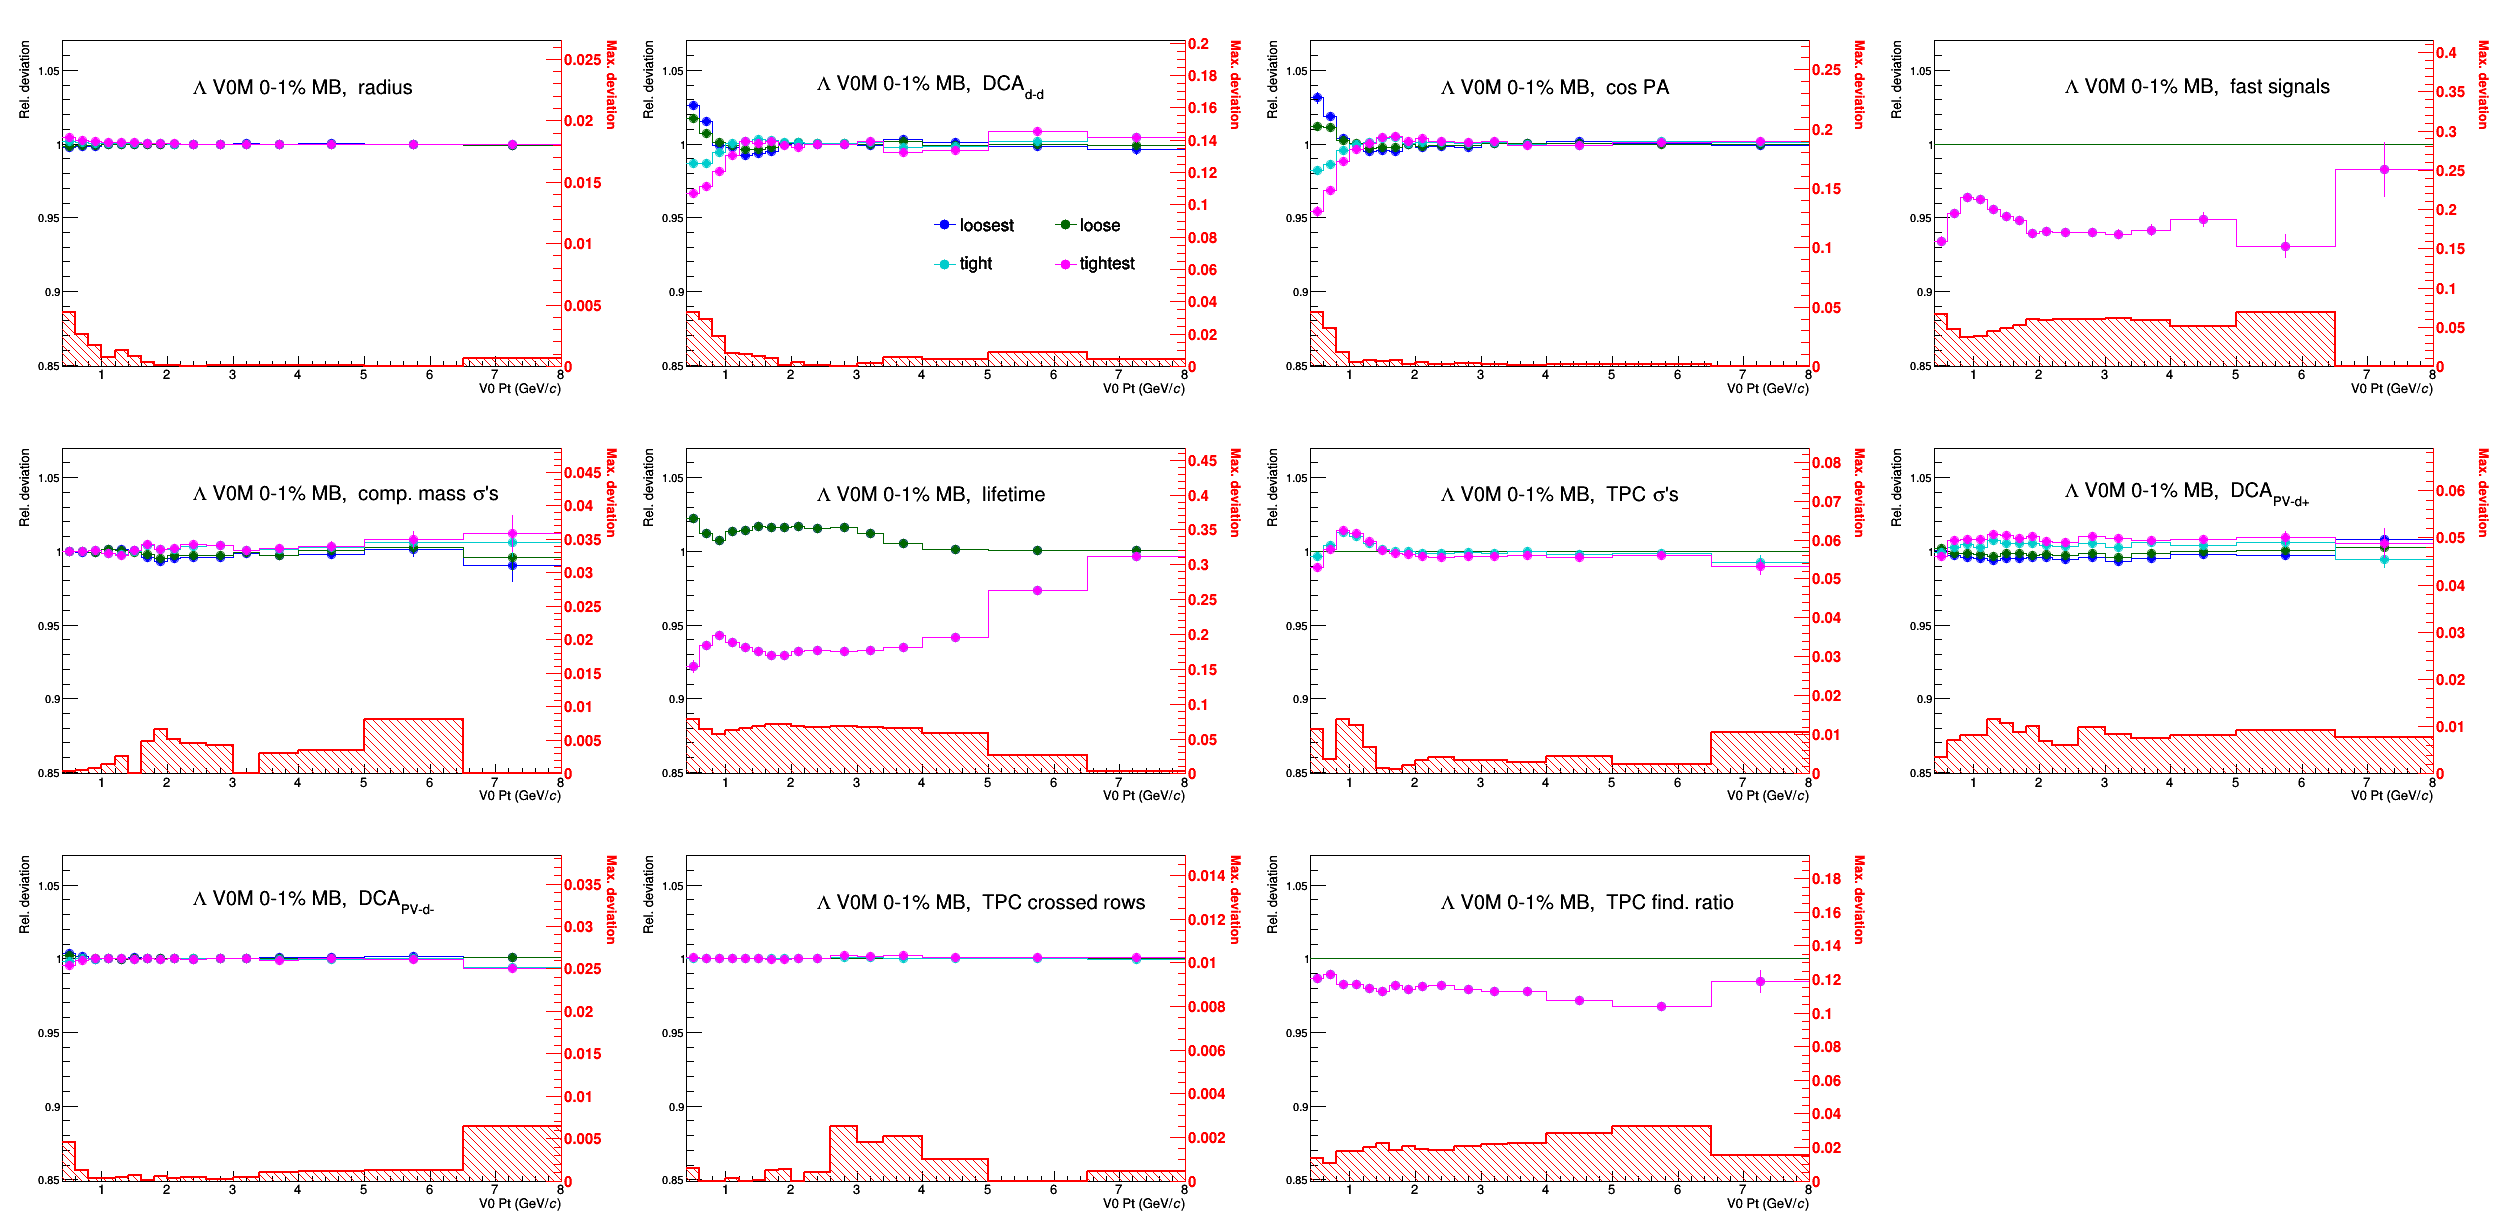
\includegraphics[width=.98\textwidth]{\imgpath/cDev_L_V0M01_MB.png}
  \caption{NEEDS TO BE REDRAWN IN CONSISTENT STYLE WITH RT CHAPTER:Deviations of the corrected spectra w.r.t.\ the different cut variations used for the \Ks . The maximum deviation is added in quadrature to the total, if it's larger than $\sigma_\mathrm{RB}$ (depicted as errorbars) from unity.}
  \label{fig:sphero:systLA}
\end{figure}

\begin{figure}[H]
  \centering
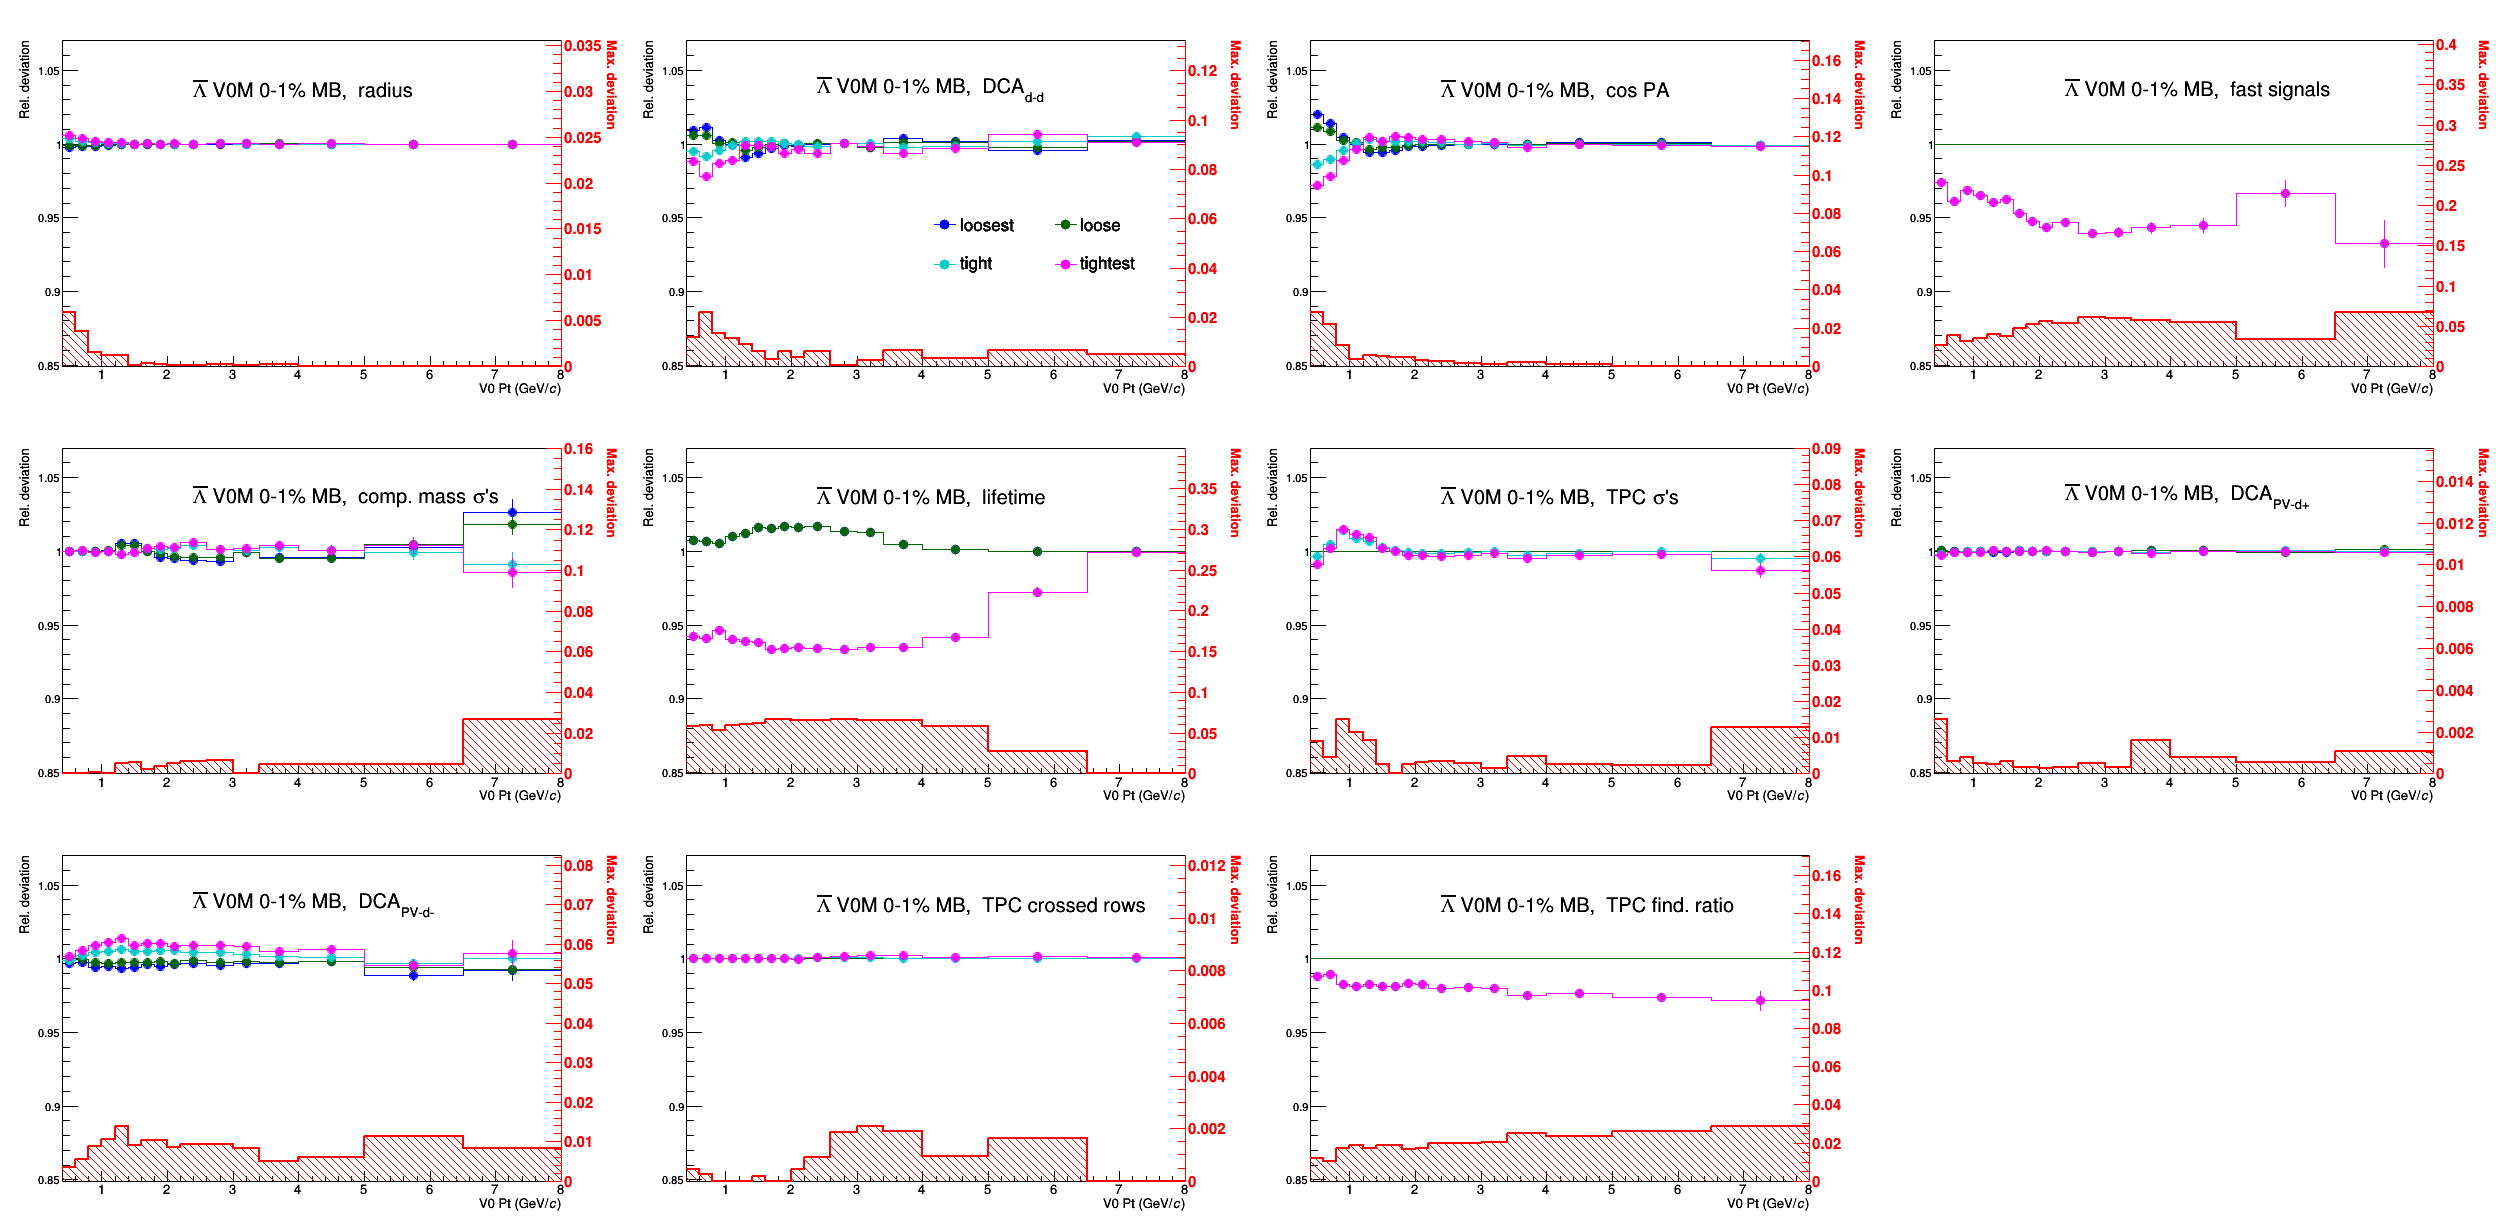
\includegraphics[width=.98\textwidth]{\imgpath/cDev_Lbar_V0M01_MB.png}
  \caption{NEEDS TO BE REDRAWN IN CONSISTENT STYLE WITH RT CHAPTER:Deviations of the corrected spectra w.r.t.\ the different cut variations used for the \Ks . The maximum deviation is added in quadrature to the total, if it's larger than $\sigma_\mathrm{RB}$ (depicted as errorbars) from unity.}
  \label{fig:sphero:systAL}
\end{figure}

\subsection{Experimental bias}

To estimate the experimental bias of the \SOPT selection, Monte Carlo closure tests were used, studying the ratios of true \pt spectra in jetty/isotropic quantiles of the true \SOPT distribution to the measured and corrected \pt spectra in quantiles of the measured \SOPT distribution.

Due to the loose DCA cuts used in the \SOPT determination, it is expected that the \VO daughters may enter its calculation. Thus, to make the predictions from simulations more comparable to the data, the \KOs, \LA, and \AL particles were included in the true \SOPT calculation. Although insufficient below $\pt < \gevc{1}$, this works well and corresponds to $1\%$ and $4\%$ discrepancies for isotropic and jetty events, respectively \cite{nassirpourShapeStrangenessTransverse2022}. 

Alternatively, as discussed further in this dissertation in the \RT measurements in Chapter~\ref{chap:rt} but not employed here, this effect could be accounted for experimentally, by making the two track sets (spherocity and \VO daughters) explicitly disjunct by enforcing a DCA cut.

\subsection{Correlation of uncertainties with \SOPT}

Correlations of several systematic uncertainties with respect to the \SOPT selection are expected. Since the ratios of jetty/isotropic results to \SOPT-unbiased ones provide important insights, it is necessary to account for these correlations in order to not overestimate the uncertainties, following the methodology described in Fig.~\ref{sec:ana:systcorr}.

Moreover, the systematic uncertainty associated with the material budget is treated as fully correlated, while assuming the reconstruction efficiency is independent of multiplicity leads to an uncorrelated uncertainty. This assumption would lead to a factor of $\sqrt{2}$ in the ratios of jetty/isotropic to \SOPT-unbiased for this uncertainty. However, in ALICE, this assumption is generally considered too conservative \cite{alicecollaborationMultiplicityDependenceLightflavor2019}, and thus this factor is dropped. The same approach is used for the uncertainty associated with the multiplicity independence of the feeddown matrix. Detailed results can be found in Appendix~\ref{app:spherosyst}.

\subsection{Summary}

The total systematic uncertainties are reported in Tab.~\ref{tab:sphero:syst} and visualised in Fig.~\ref{fig:sphero:systtot}. The dominant contributions are, in no specific order, selection cuts, experimental bias, signal extraction, and the enforcement of signals from fast detectors to prevent track pile-up.

\begin{table}[H]
\centering
\caption{The most relevant systematic uncertainties for the long-lived particles \KOs and \LA(\AL) as a function of \SOPT. ``HM'' in this table represents the \SOPT-unbiased spectra. Uncertainties are pt-dependent, and the ranges listed represents the minimum-maximum values presented in the final spectra (see text for details). }
\label{tab:sphero:syst}
\begin{tabular}{|l|lllll|}
\hline
\multicolumn{1}{|r|}{Topology:}              & Jetty     & Iso       & HM        & Jetty/HM       & Iso/HM      \\ \hline

\multicolumn{6}{l}{\parbox[b][1.2em]{1em}{K$^0_\mathrm{S}$}} \\
\hline
Selection cuts        & 3\%    & 3--4\%     & 3--4\%     & Negl.          & 1\%          \\
Track pile--up        & 1\% & 1--3\% & 1\% & 0--2\% & 0--2\%   \\
Signal extraction     & 1--3\%     & 1--3\%     & 1--3\%     & Negl. & Negl. \\
Efficiency            & 2\%    & 2\%    & 2\%    & 2\%         & 2\%         \\
Material budget       & 4\%    & 4\%    & 4\%    & --              & --              \\
Experimental bias     & 4\%    & 1\%    & --         & 4\%         & 1\%         \\ \hline
Total uncertainty     & 7\%    & 6--7\%\%   & 5--6\%     & 5\%         & 2--3\%          \\ \hline
\multicolumn{6}{l}{\parbox[b][1.2em]{1em}{$\Lambda$($\overline{\Lambda})$}} \\
\hline
Selection cuts & 1--5\%     & 2--6\%     & 4--5\%     & 0--1\%          & 0--3\%          \\
Track pile--up        & 4--5\% & 5\% & 3--5\% & 0--1.5\% & 0--1\%   \\
Signal extraction     & 2--6\%     & 2--6\%     & 2--6\%     & 0--2\%          & 0--1\%          \\
Feed-down correction   & 1.0--1.5\% & 1.0--1.5\% & 1.0--1.5\% & Negl. & Negl. \\
Efficiency            & 2\%    & 2\%    & 2\%    & 2\%         & 2\%         \\
Material budget       & 4\%    & 4\%    & 4\%    & --              & --              \\
Experimental bias     & 4\%    & 1\%    & --         & 4\%         & 1\%         \\ \hline
Total uncertainty     & 8--10\%    & 8--9\%     & 7--9\%     & 5\%         & 3--4\%          \\ \hline
\end{tabular}
\end{table}

\begin{figure}[H]
\centering
\subfloat[][]{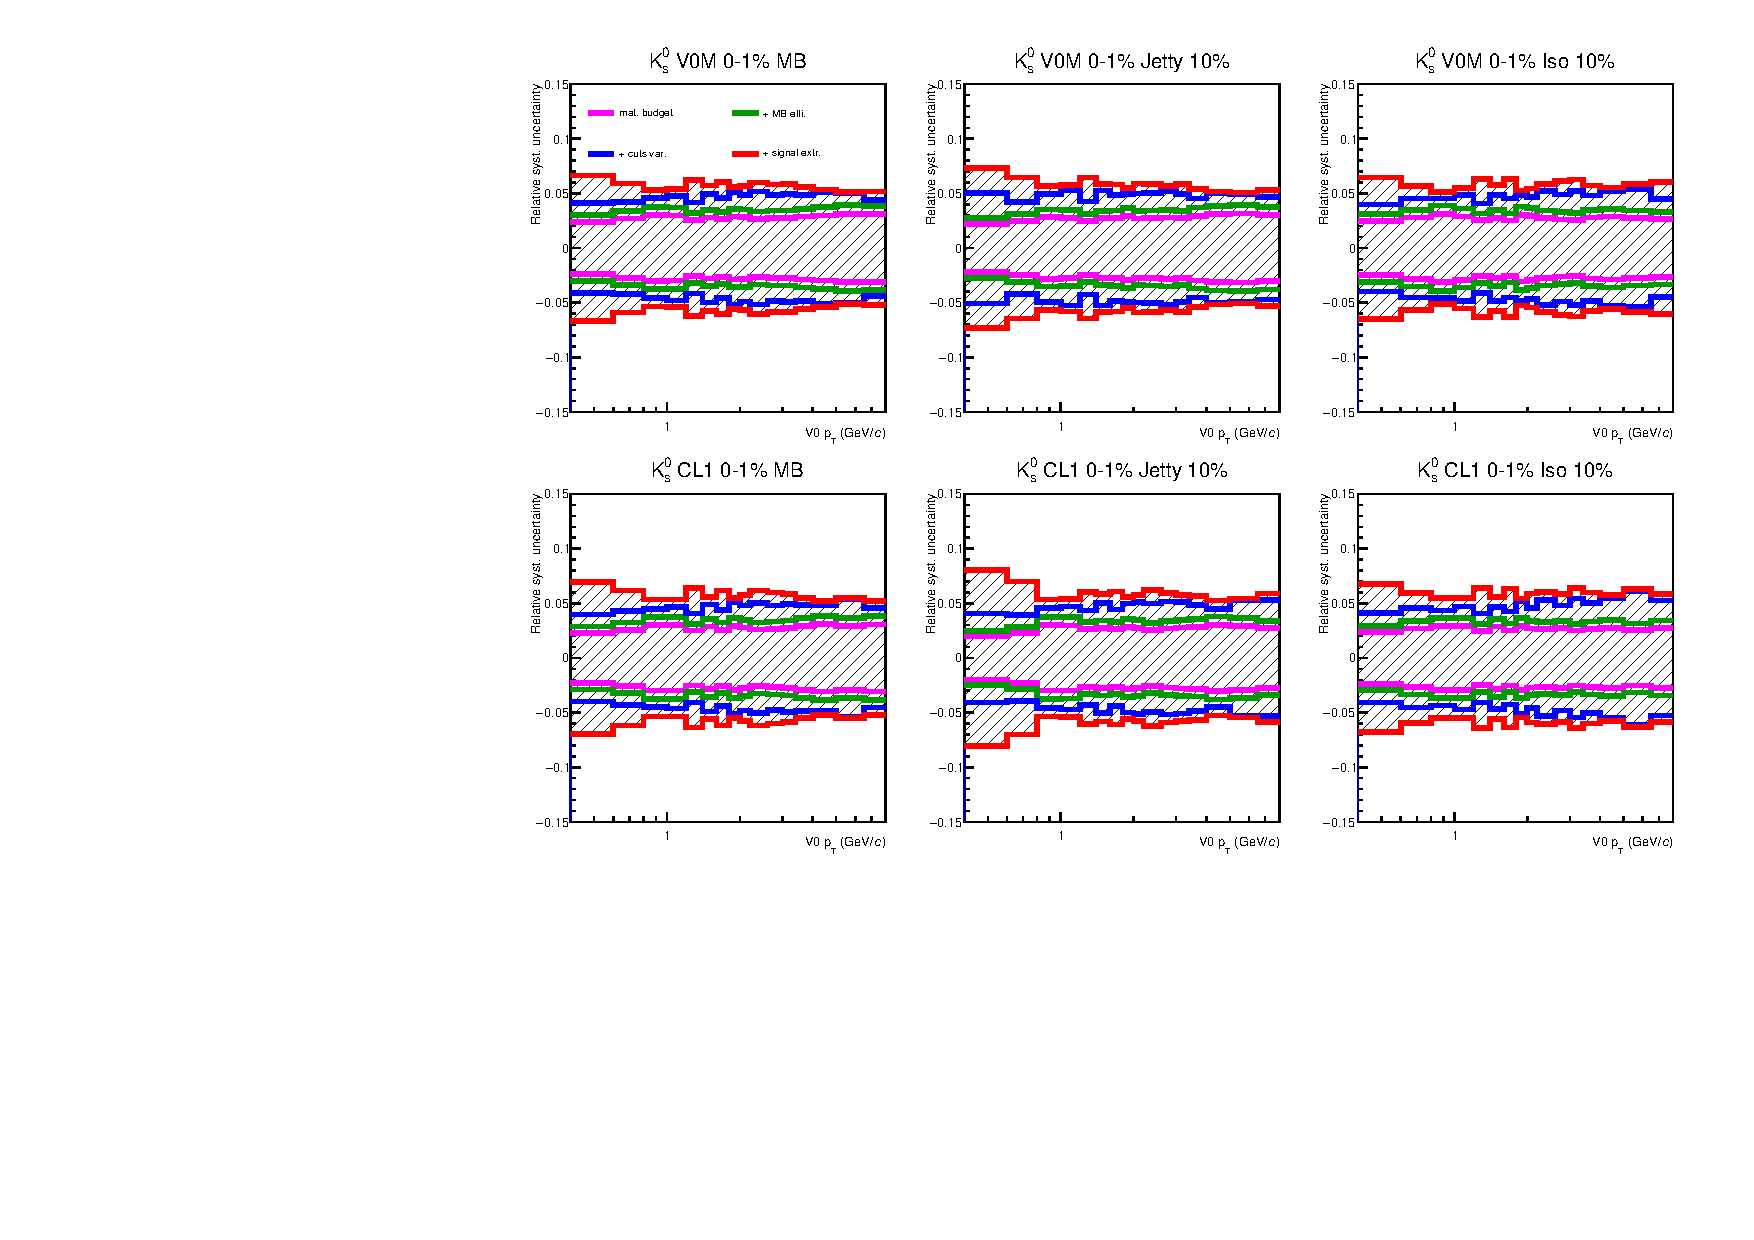
\includegraphics[height=.3\textheight]{\imgpath/k0s_sys.pdf}}\\
\subfloat[][]{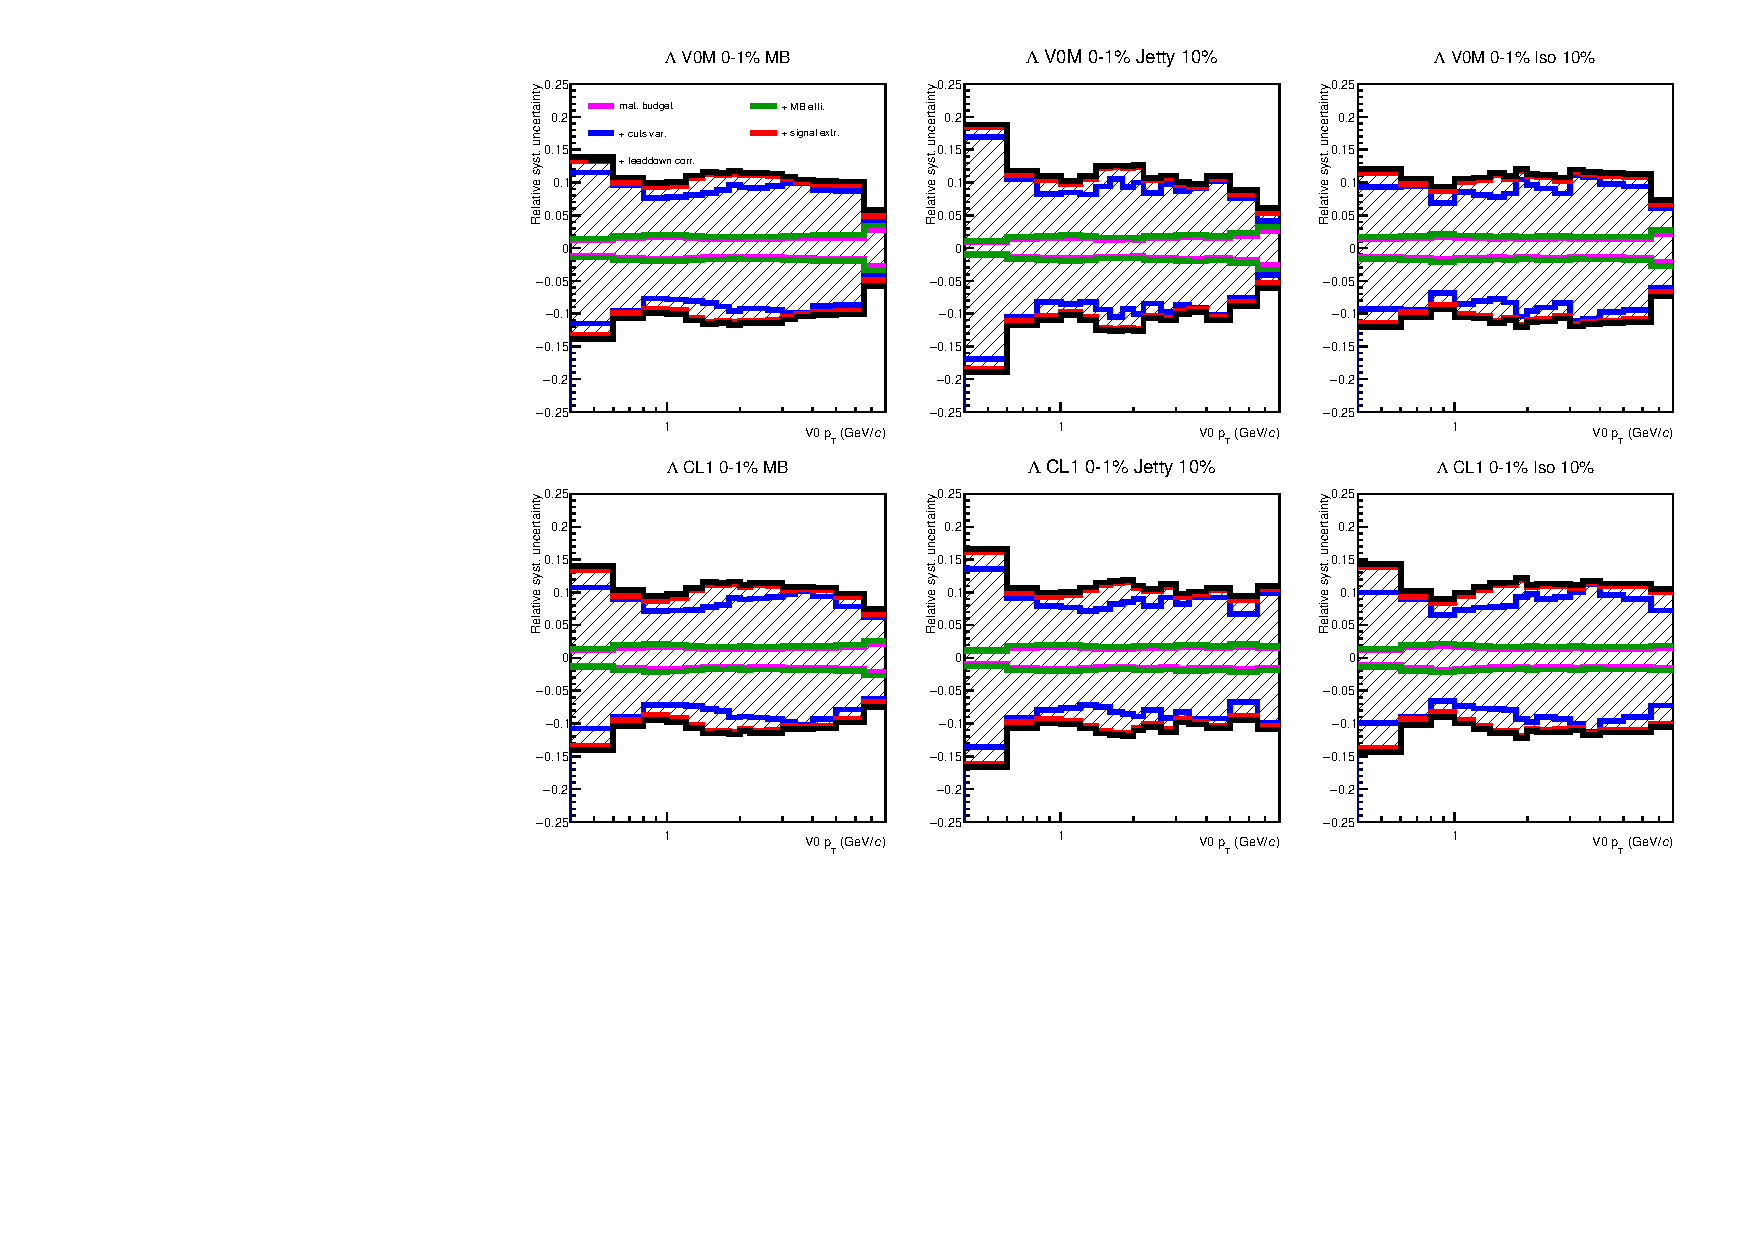
\includegraphics[height=.3\textheight]{\imgpath/l_sys.pdf}}\\
%\subfloat[][]{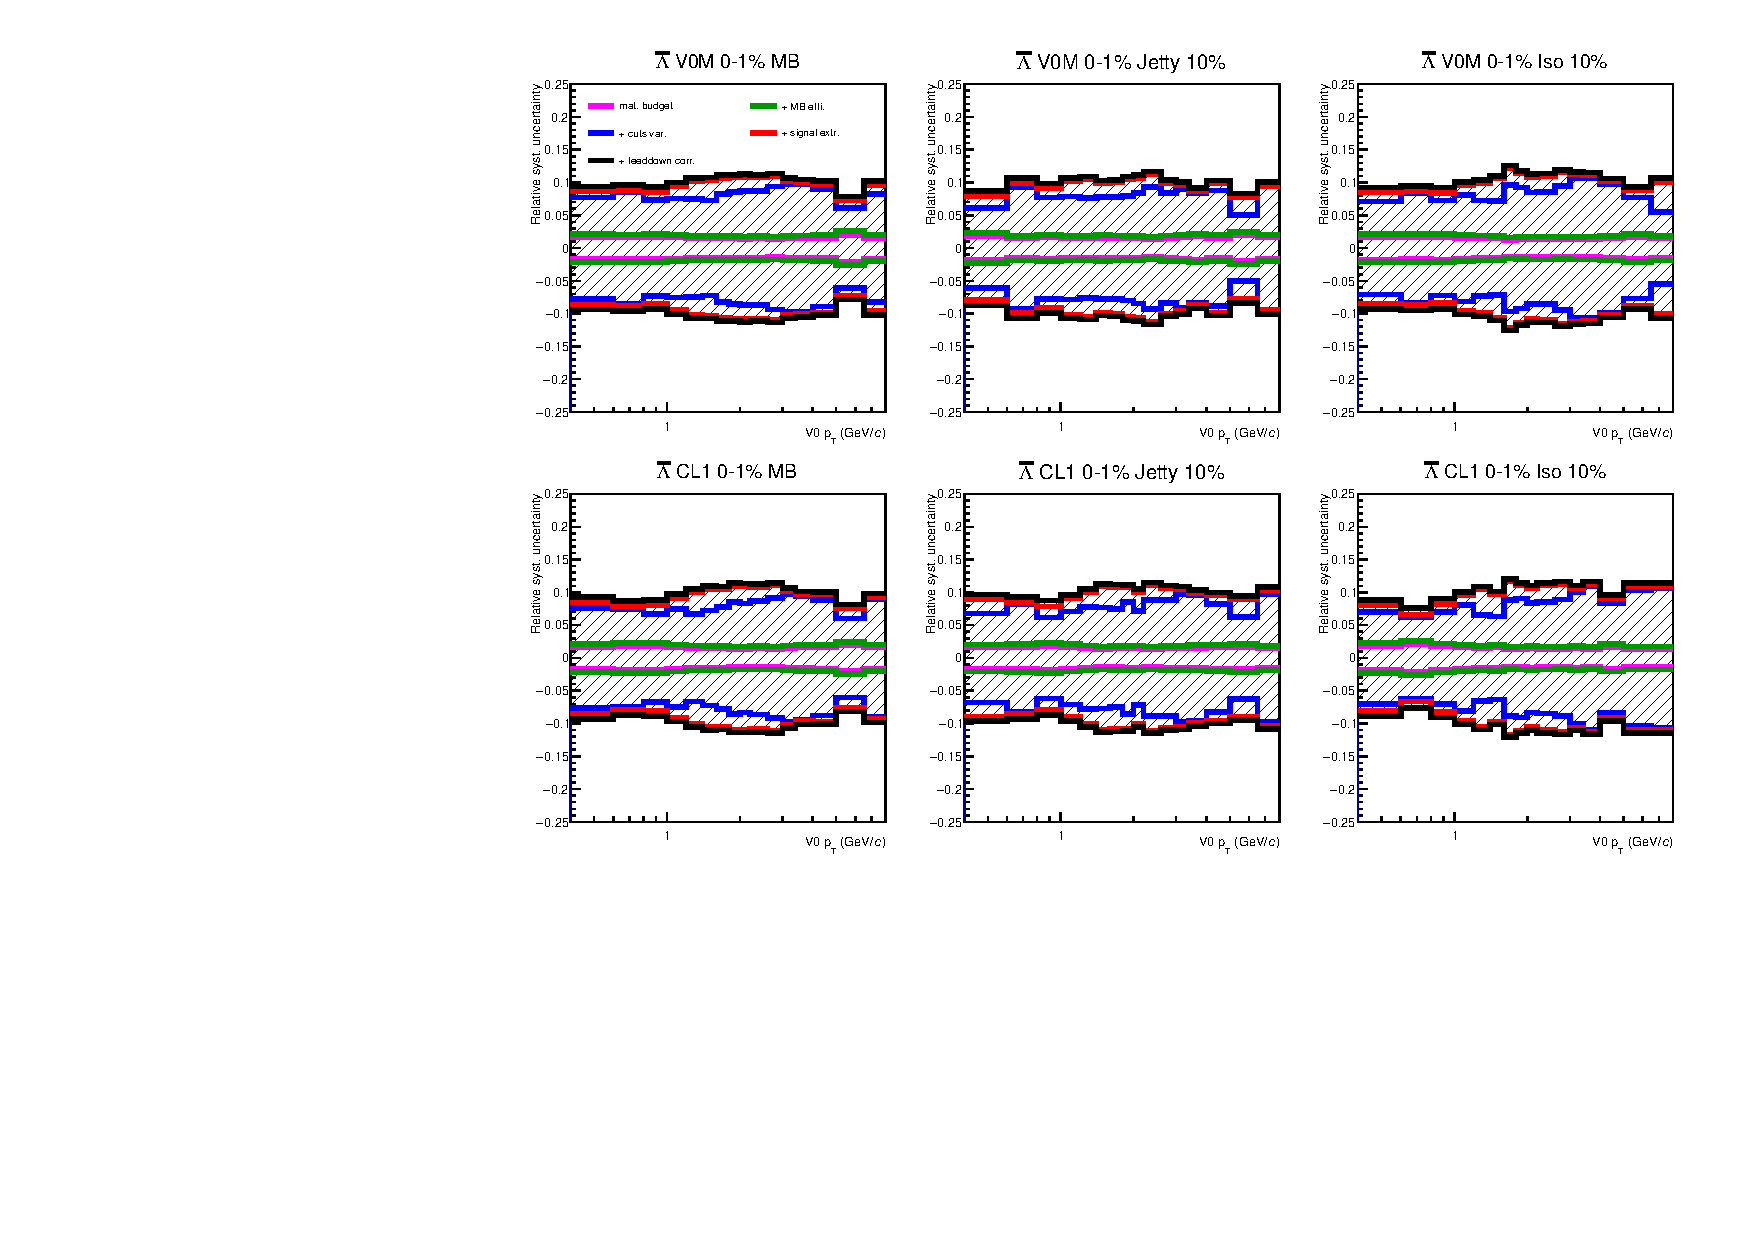
\includegraphics[height=.3\textheight]{\imgpath/lbar_sys.pdf}}\\
\caption{NEEDS TO BE REDRAWN IN CONSISTENT STYLE WITH RT CHAPTER: Total relative systematic uncertainty and individual contributions for the \KOs, \LA, and \AL .}
\label{fig:sphero:systtot}
\end{figure}


\section{Transverse momentum spectra vs. \SOPT}

The corrected spectra in \VOM and \NSPD high-multiplicity events and the dependence on spherocity for the \KOs and \LA + \AL can be seen in Fig.~\ref{fig:sphero:k0spt} and Fig.~\ref{fig:sphero:lpt}, respectively.  The trends observed in the spectra are consistent between \KOs and \LA and indicate a significant hardening (softening) in the low (high) spherocity selection, relative to the inclusive high-multiplicity event class. These trends are qualitatively generally well captured by all included model predictions, favouring Pythia 8 Ropes. Particularly, EPOS LHC overestimates the yields and Pythia 8 Monash fails in describing the \LA \pt spectra.

The seperation between jetty and isotropic events is more pronounced in the \NSPD high-multiplicity events, and shows significant difference in the spectra slopes rather than just an offset, which is somewhat the case for the \VOM events.

\begin{figure}[H]%
\centering%
\subfloat[][]{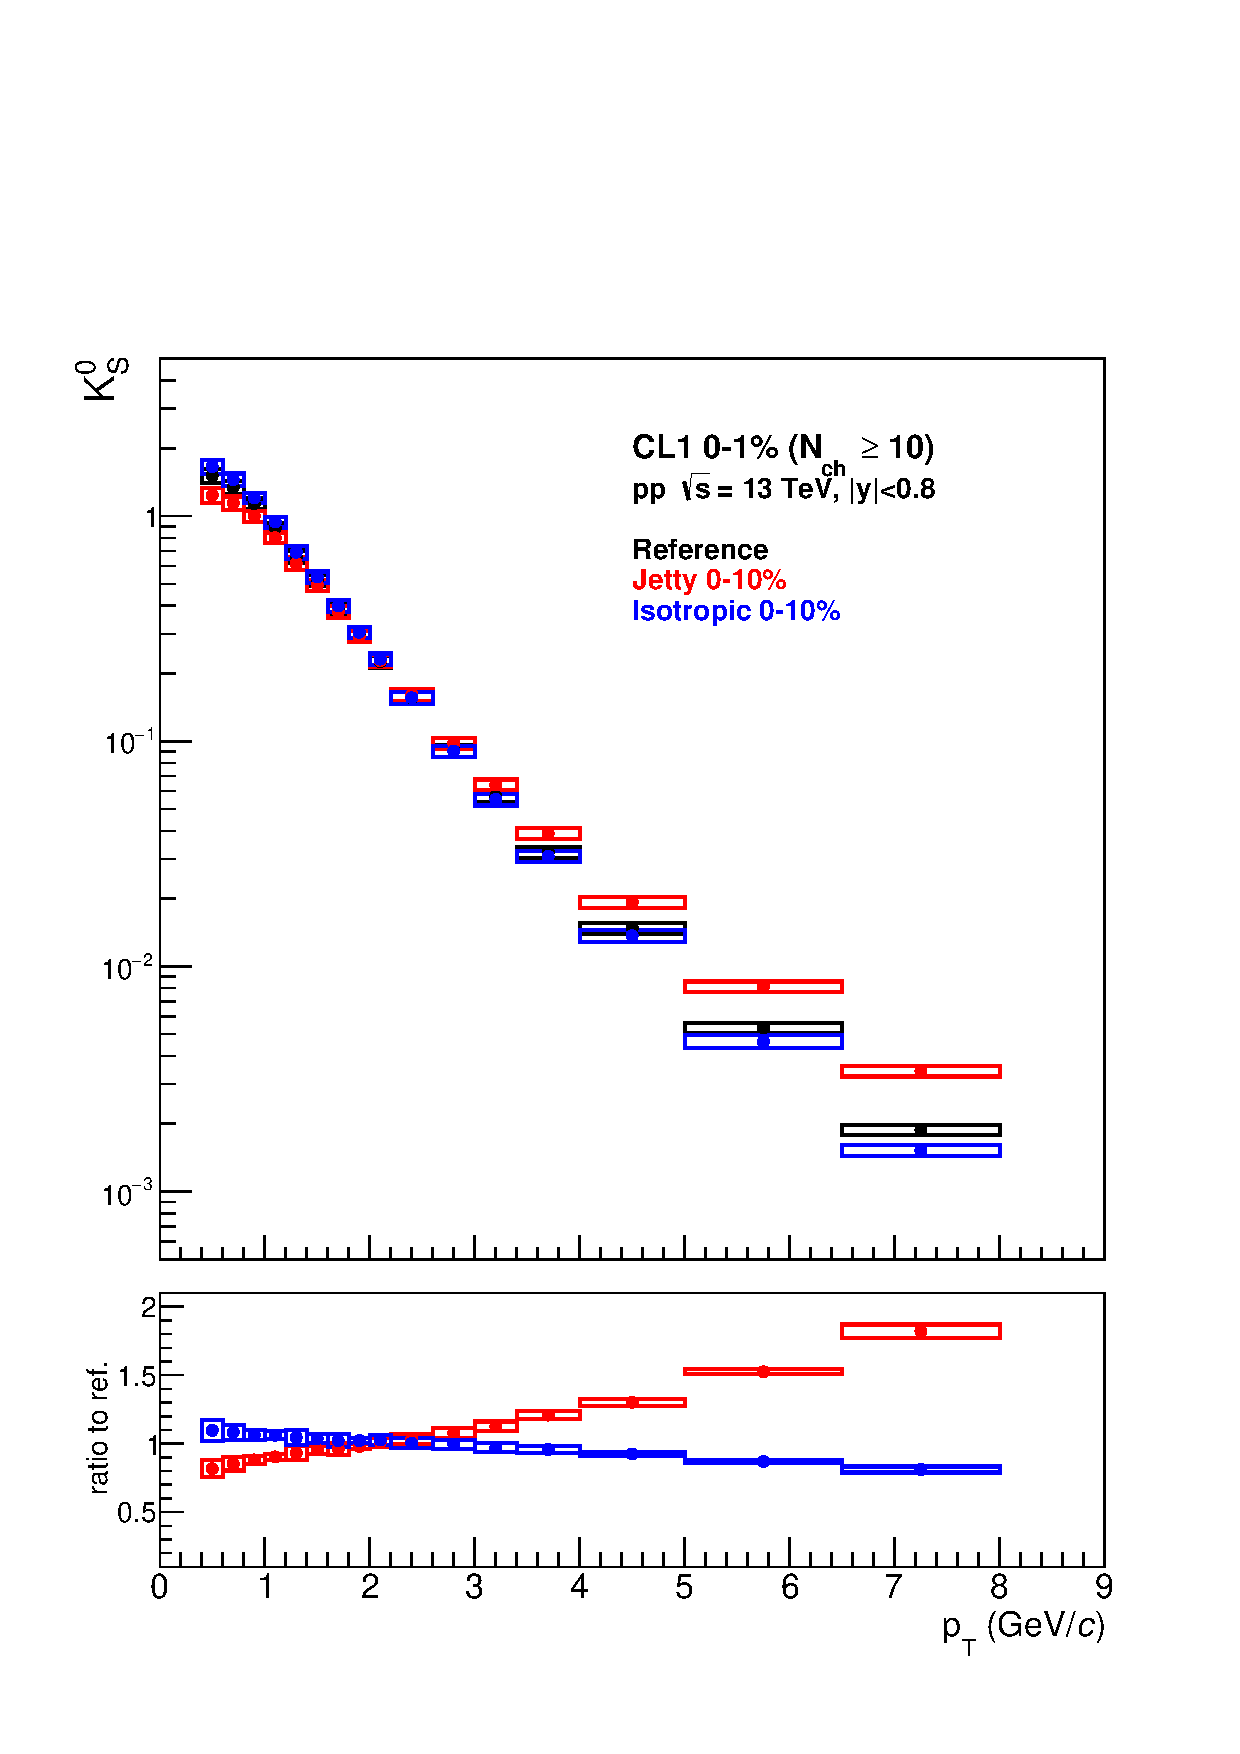
\includegraphics[width=.33\textwidth]{\imgpath/sp_K0s_NCharged01_spher10.pdf}}
\subfloat[][]{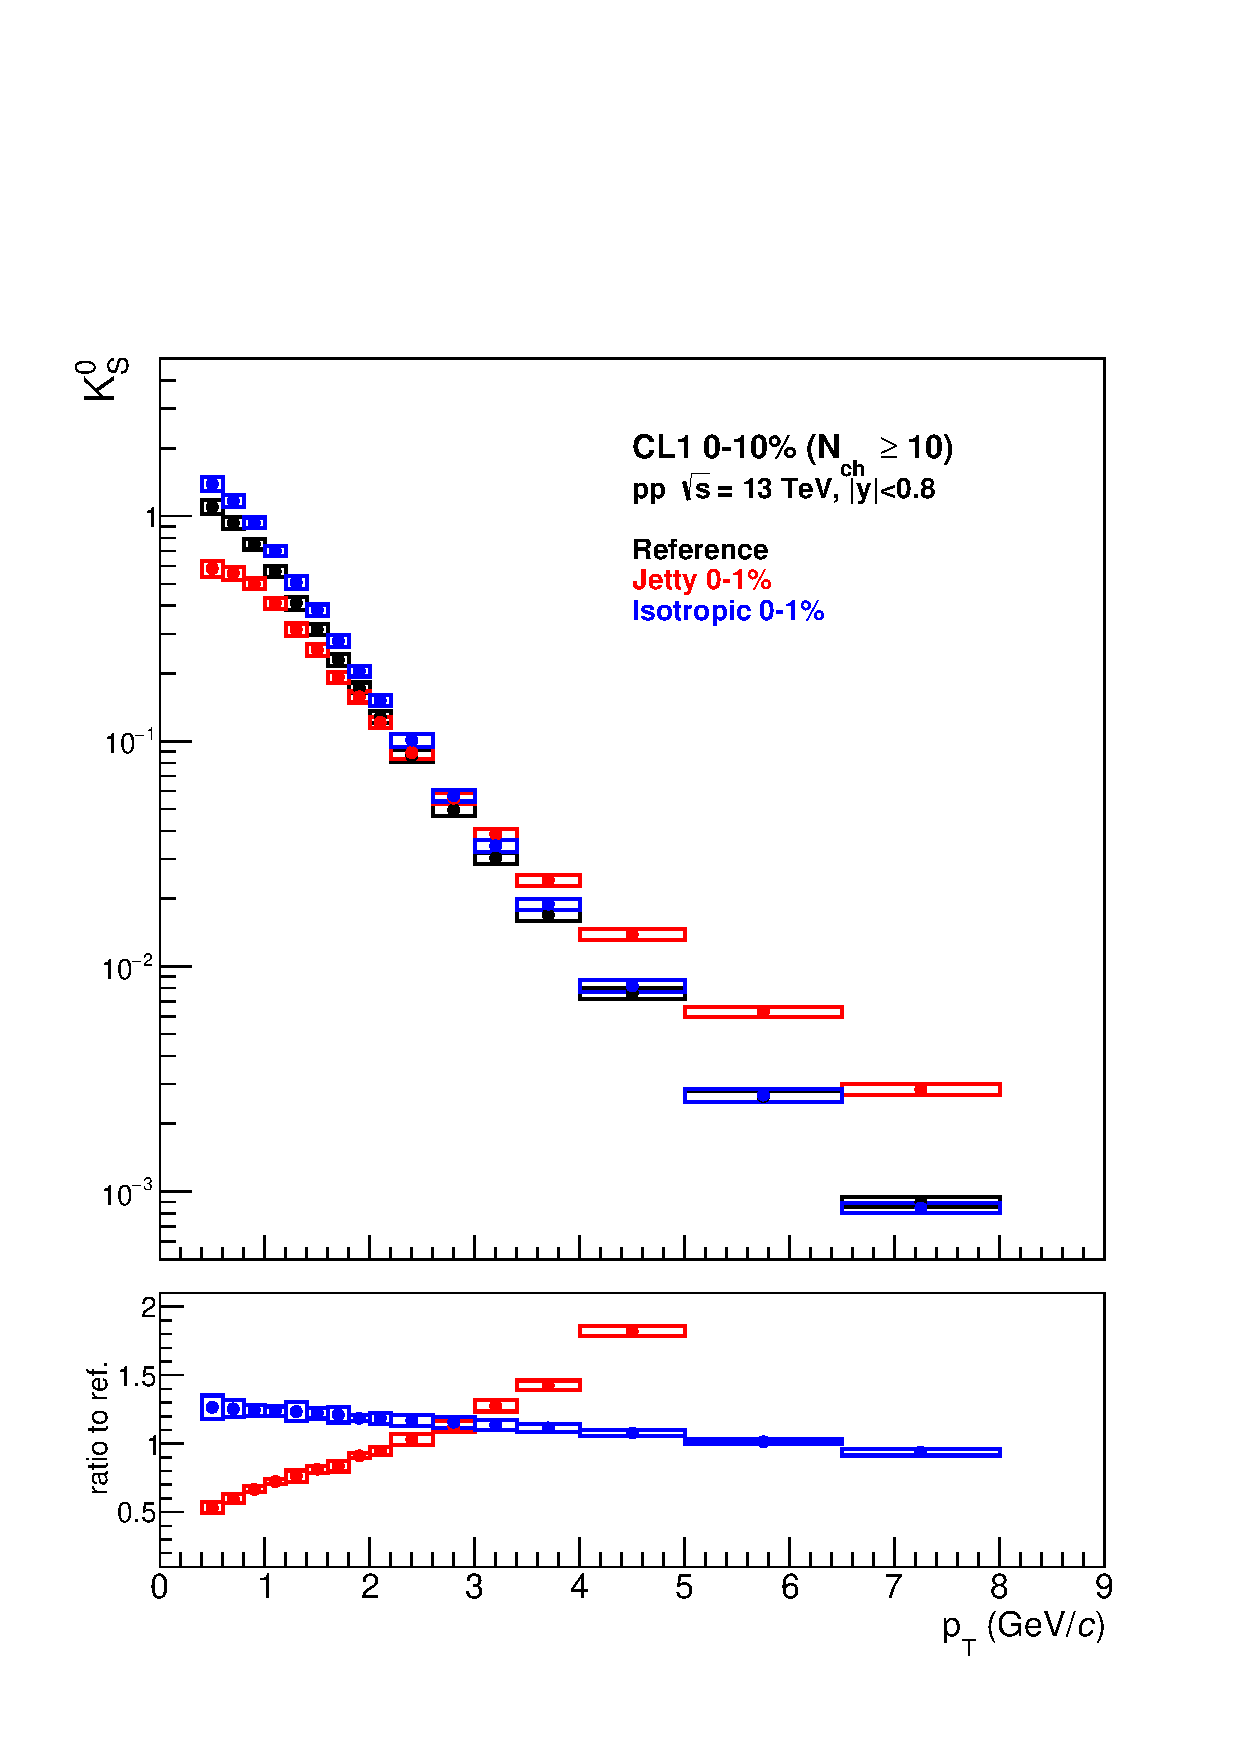
\includegraphics[width=.33\textwidth]{\imgpath/sp_K0s_NCharged_spher1.pdf}}
\subfloat[][]{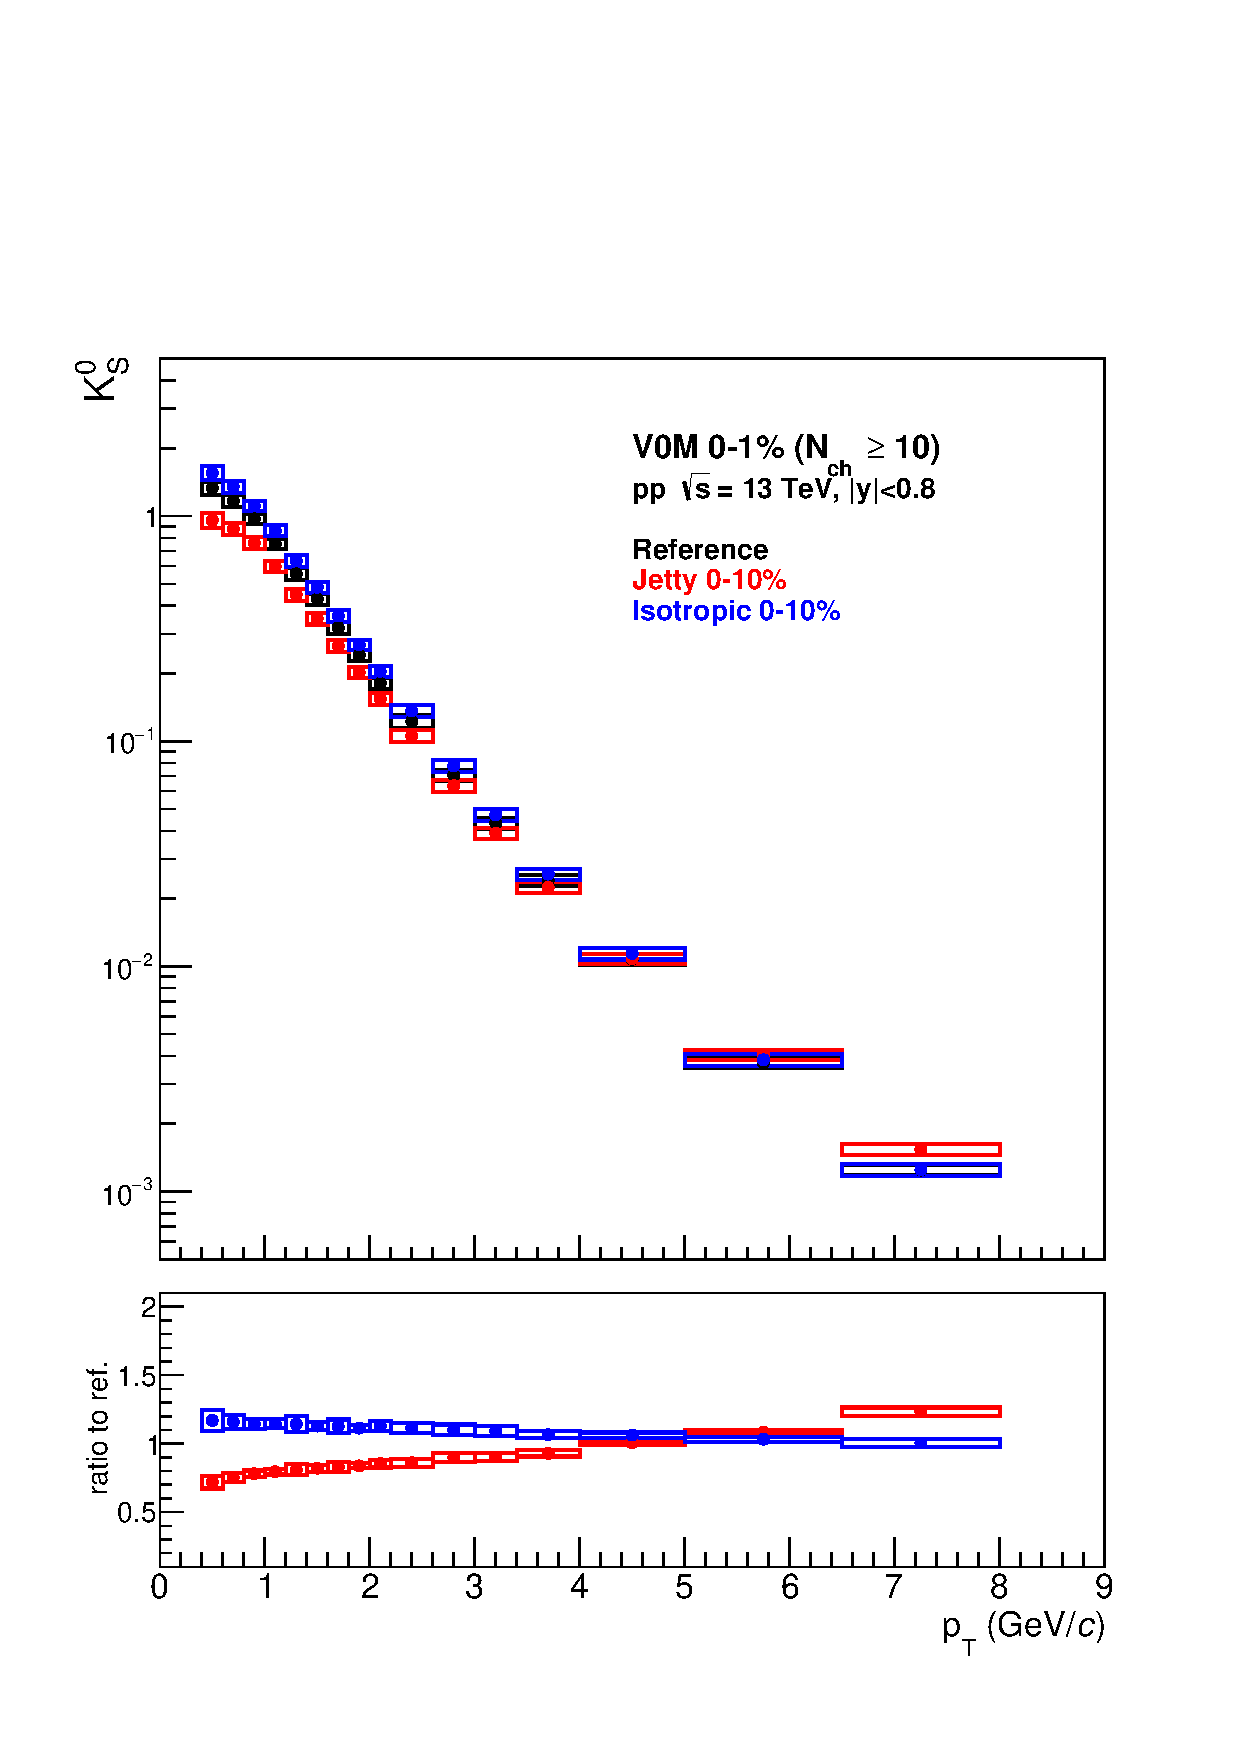
\includegraphics[width=.33\textwidth]{\imgpath/sp_K0s_V0M01_spher10.pdf}}
\caption{Transverse momentum spectra of \KOs in high-multiplicity jetty (red) and isotropic (blue) events of pp collisions at \sppt{13} measured in the \textbf{(a)} \NSPD I, \textbf{(b)} \NSPD I-III, and \textbf{(c)} \VOM I event classes. The bottom panels display ratios to the \SOPT-unbiased spectra. Statistical and systematic uncertainties are indicated with error bars and boxes, respectively. (\textit{Needs to be redrawn to also show MC})}
\label{fig:sphero:k0spt}
\end{figure}

\begin{figure}[H]%
\centering%
\subfloat[][]{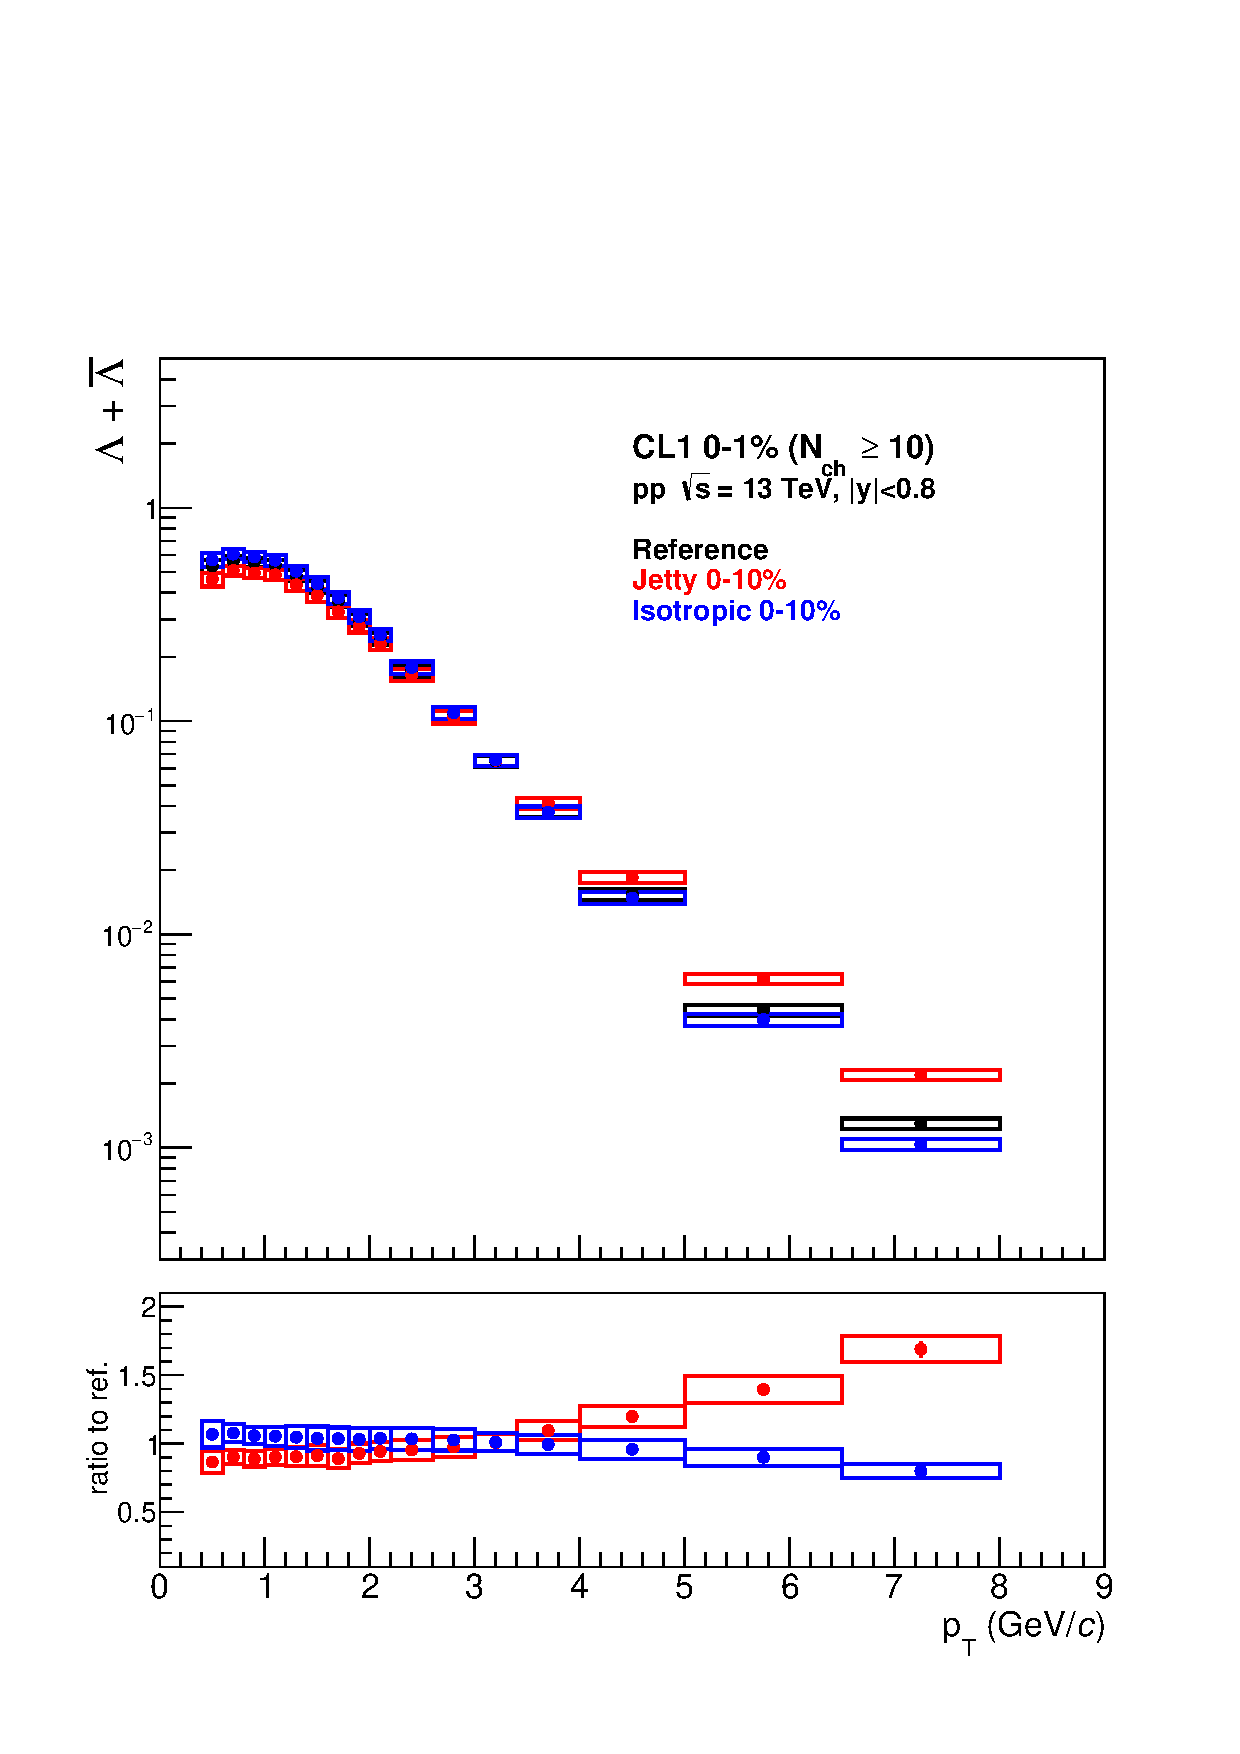
\includegraphics[width=.33\textwidth]{\imgpath/sp_LLbar_NCharged01_spher10.pdf}}
\subfloat[][]{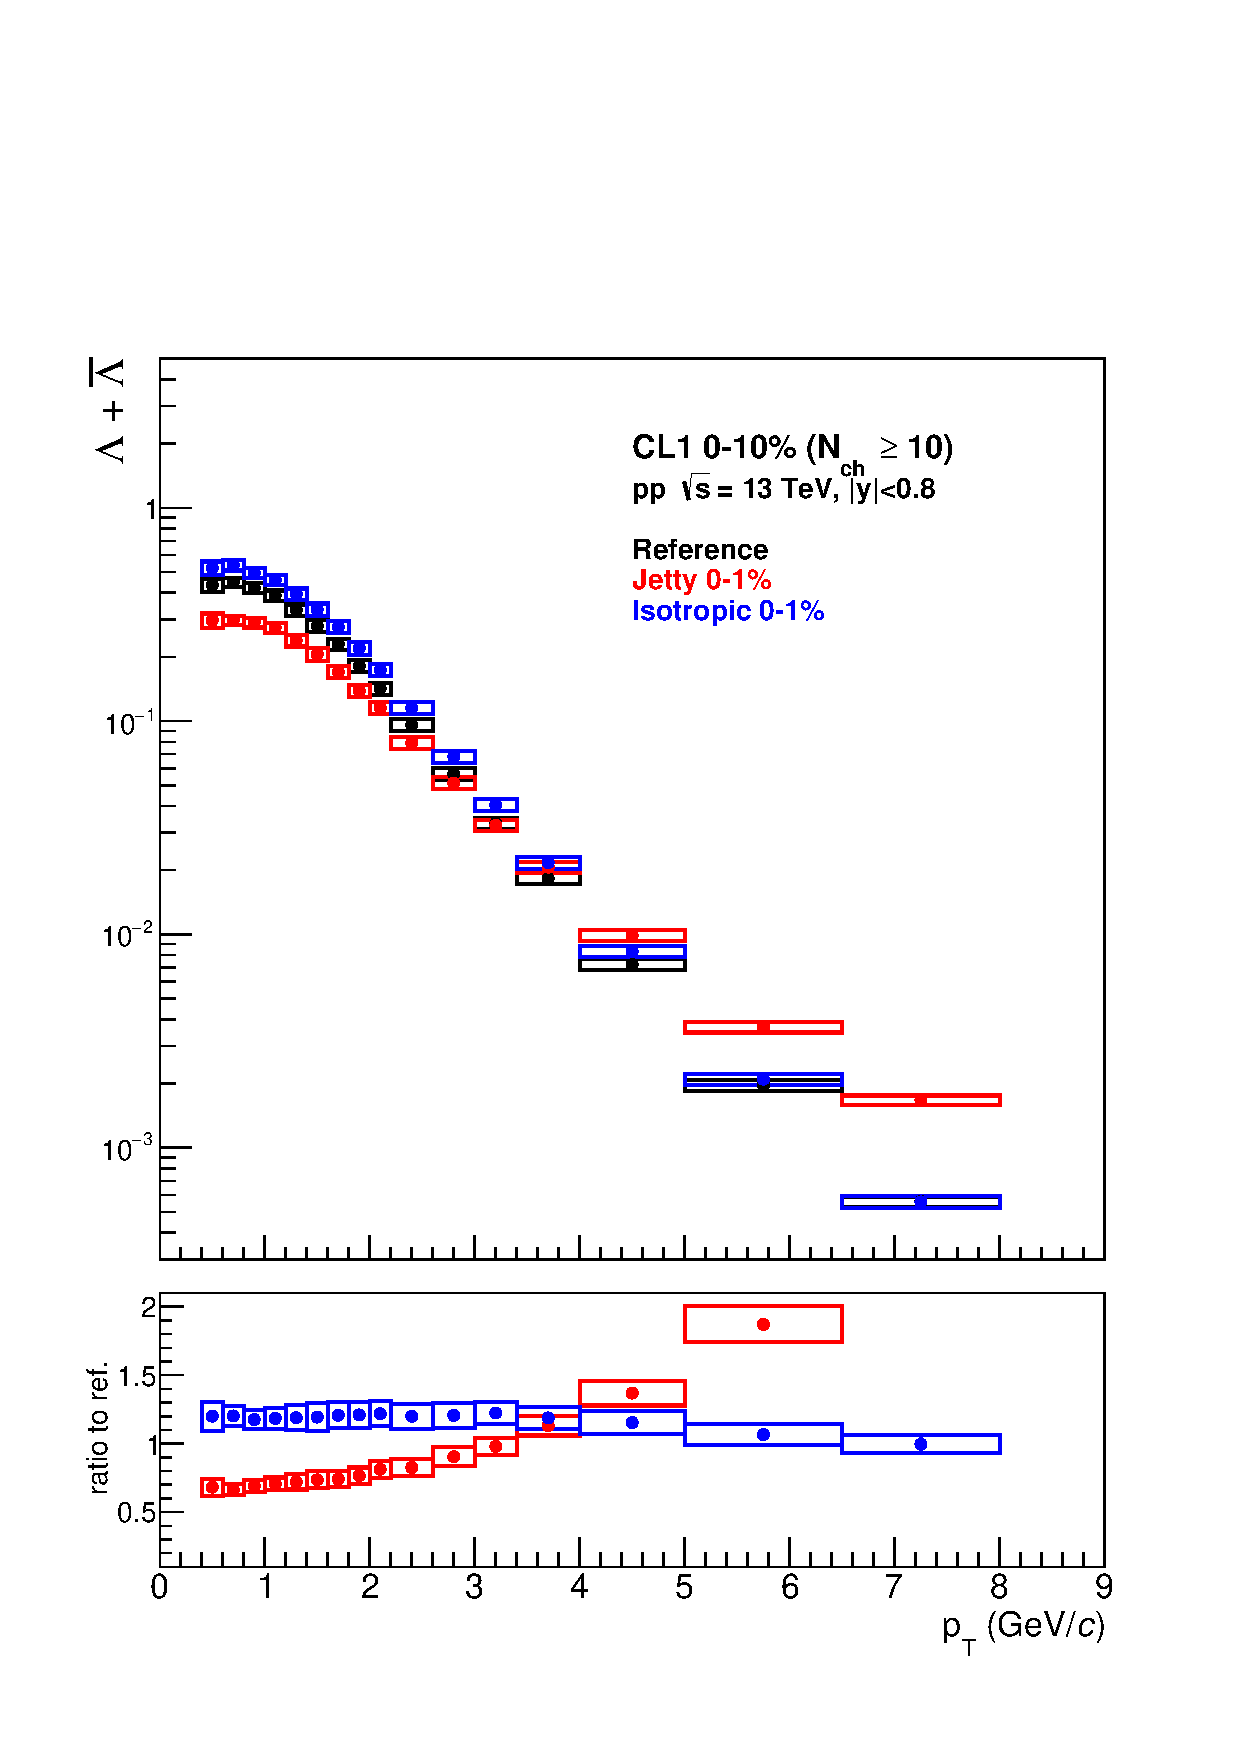
\includegraphics[width=.33\textwidth]{\imgpath/sp_LLbar_NCharged_spher1.pdf}}
\subfloat[][]{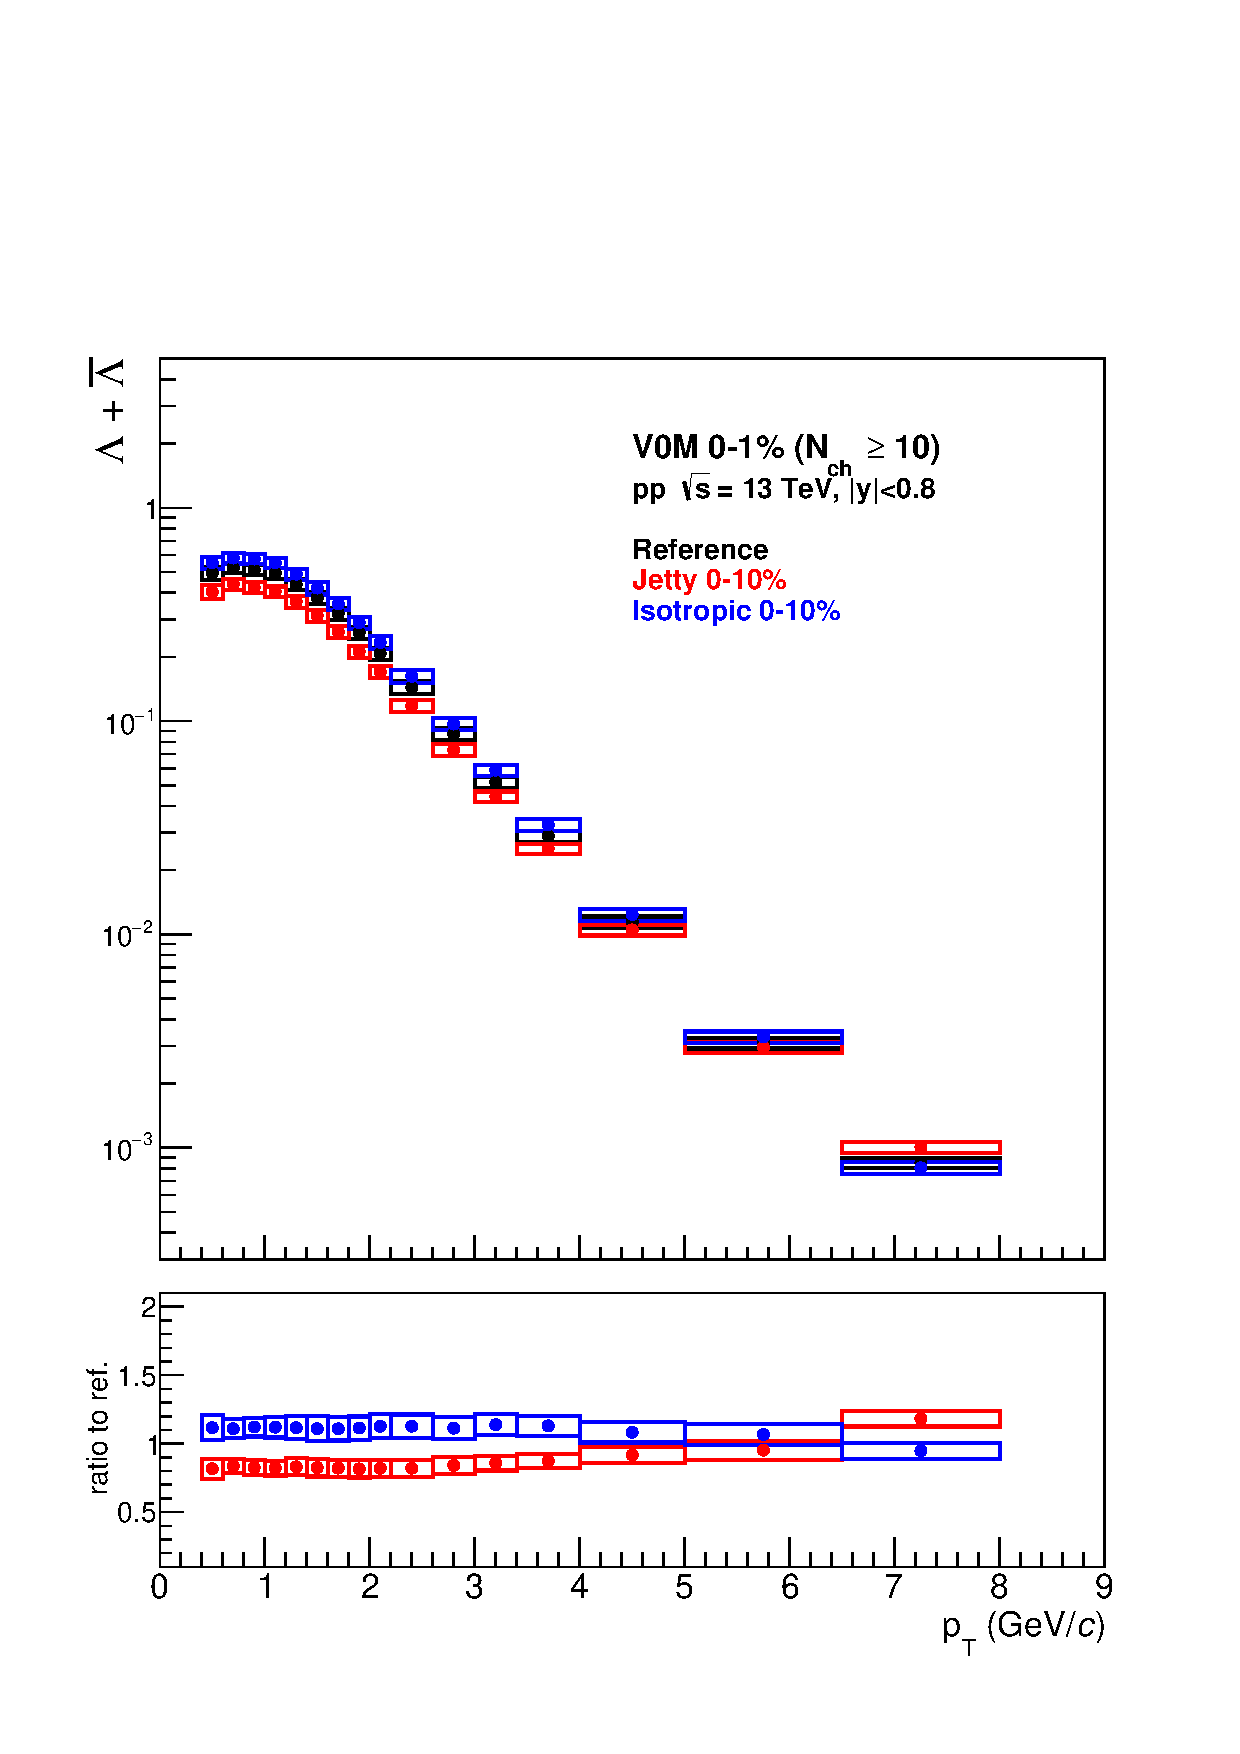
\includegraphics[width=.33\textwidth]{\imgpath/sp_LLbar_V0M01_spher10.pdf}}
\caption{Transverse momentum spectra of \LA+\AL in high-multiplicity jetty (red) and isotropic (blue) events of pp collisions at \sppt{13} measured in the \textbf{(a)} \NSPD I, \textbf{(b)} \NSPD I-III, and \textbf{(c)} \VOM I event classes. The bottom panels display ratios to the \SOPT-unbiased spectra. Statistical and systematic uncertainties are indicated with error bars and boxes, respectively. (\textit{Needs to be redrawn to also show MC and be cut off from 1 GeV.})}
\label{fig:sphero:lpt}
\end{figure}

\subsection{Ratios of neutral kaons to charged kaons}

To verify the robustness of \SOPT as an event observable, the \pt spectra of neutral and charged kaons are compared in the \NSPD I and \VOM I classes. The ratios exhibit no dependence on \SOPT and are consistent with unity, according to expectations. The slight depletion of \KOs in the \NSPD I class is interpreted as the multiplicity selection bias due to requiring a large number of charged tracks at mid-rapidity, and is also reproducible by simulations. The ratios are shown in Fig.~\ref{fig:sphero:ktok}.

\begin{figure}[H]%
\centering%
\subfloat[][]{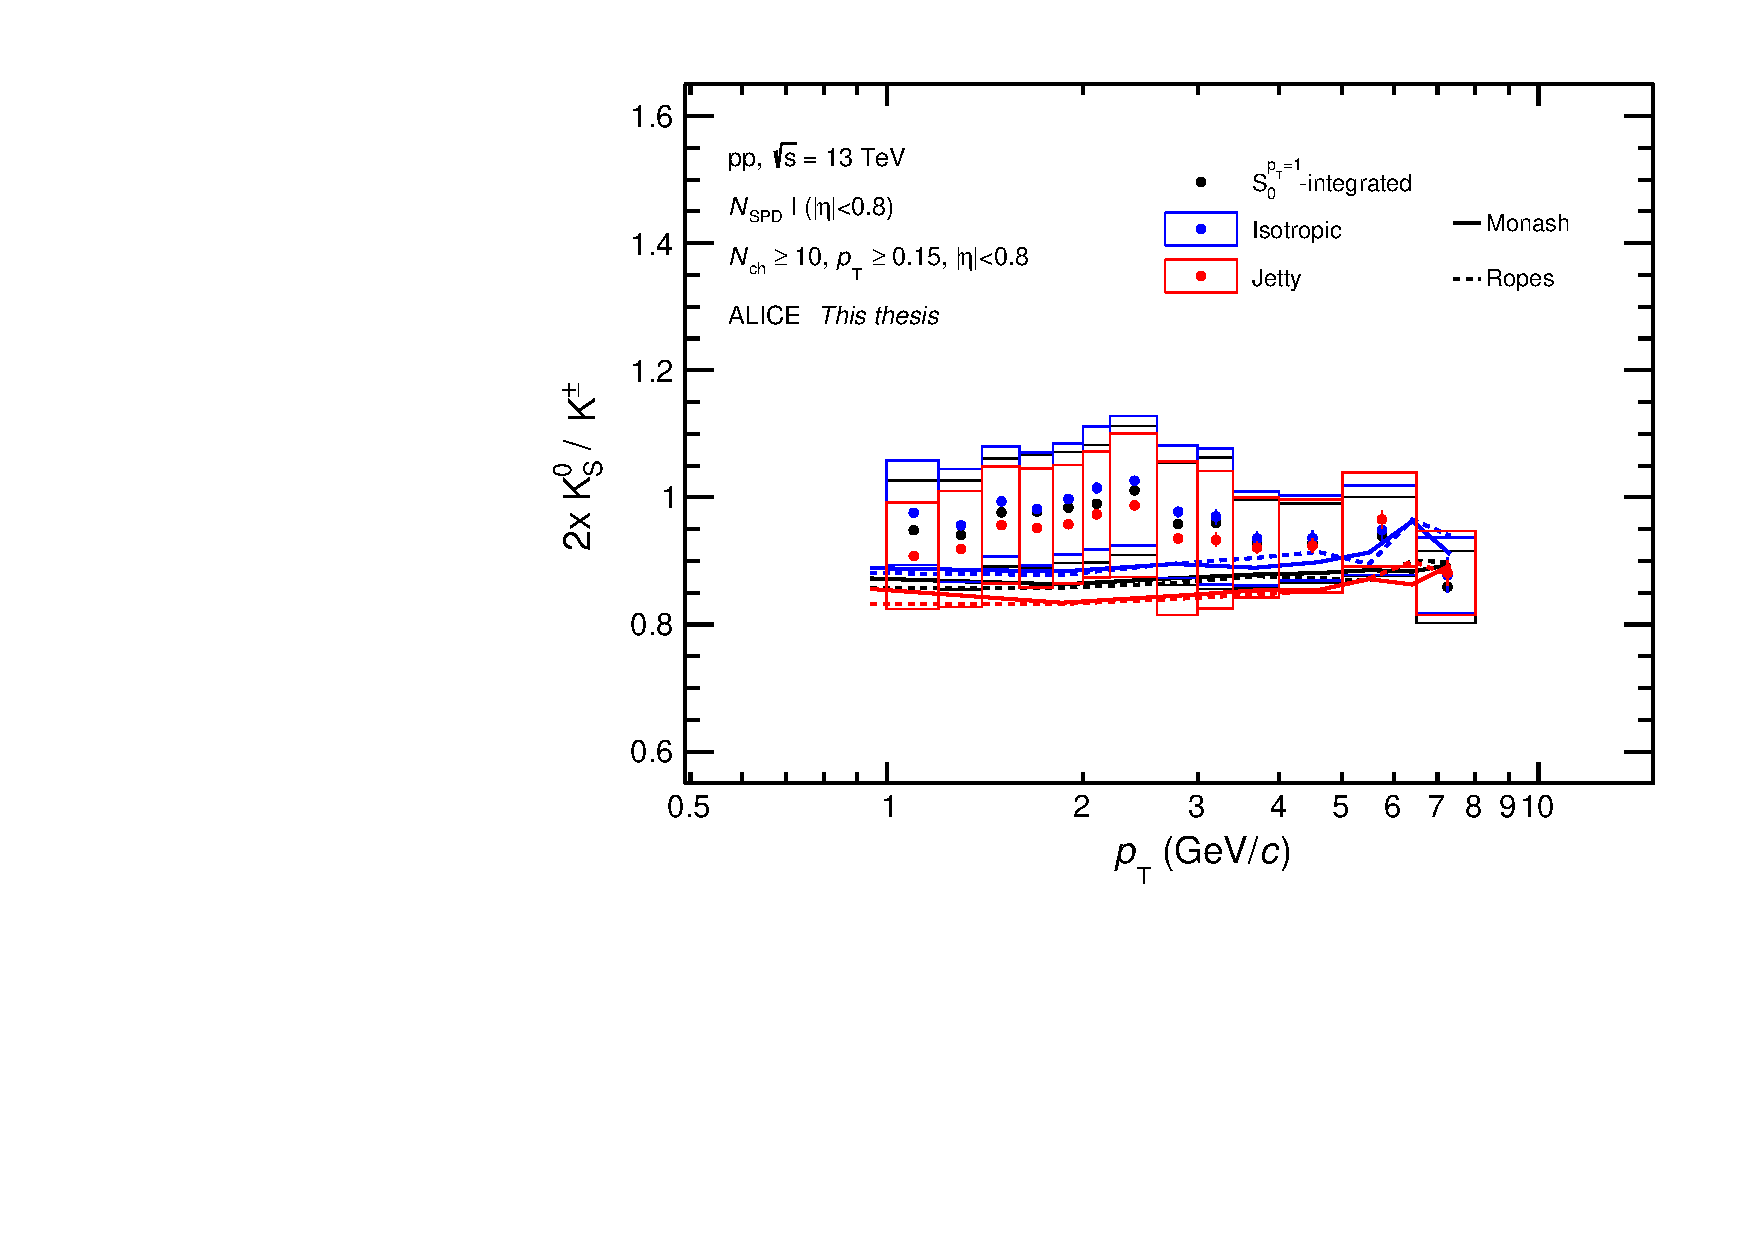
\includegraphics[width=.4\textwidth]{\imgpath/KtoK_NCharged01_spher10.pdf}}\hspace{1em}
\subfloat[][]{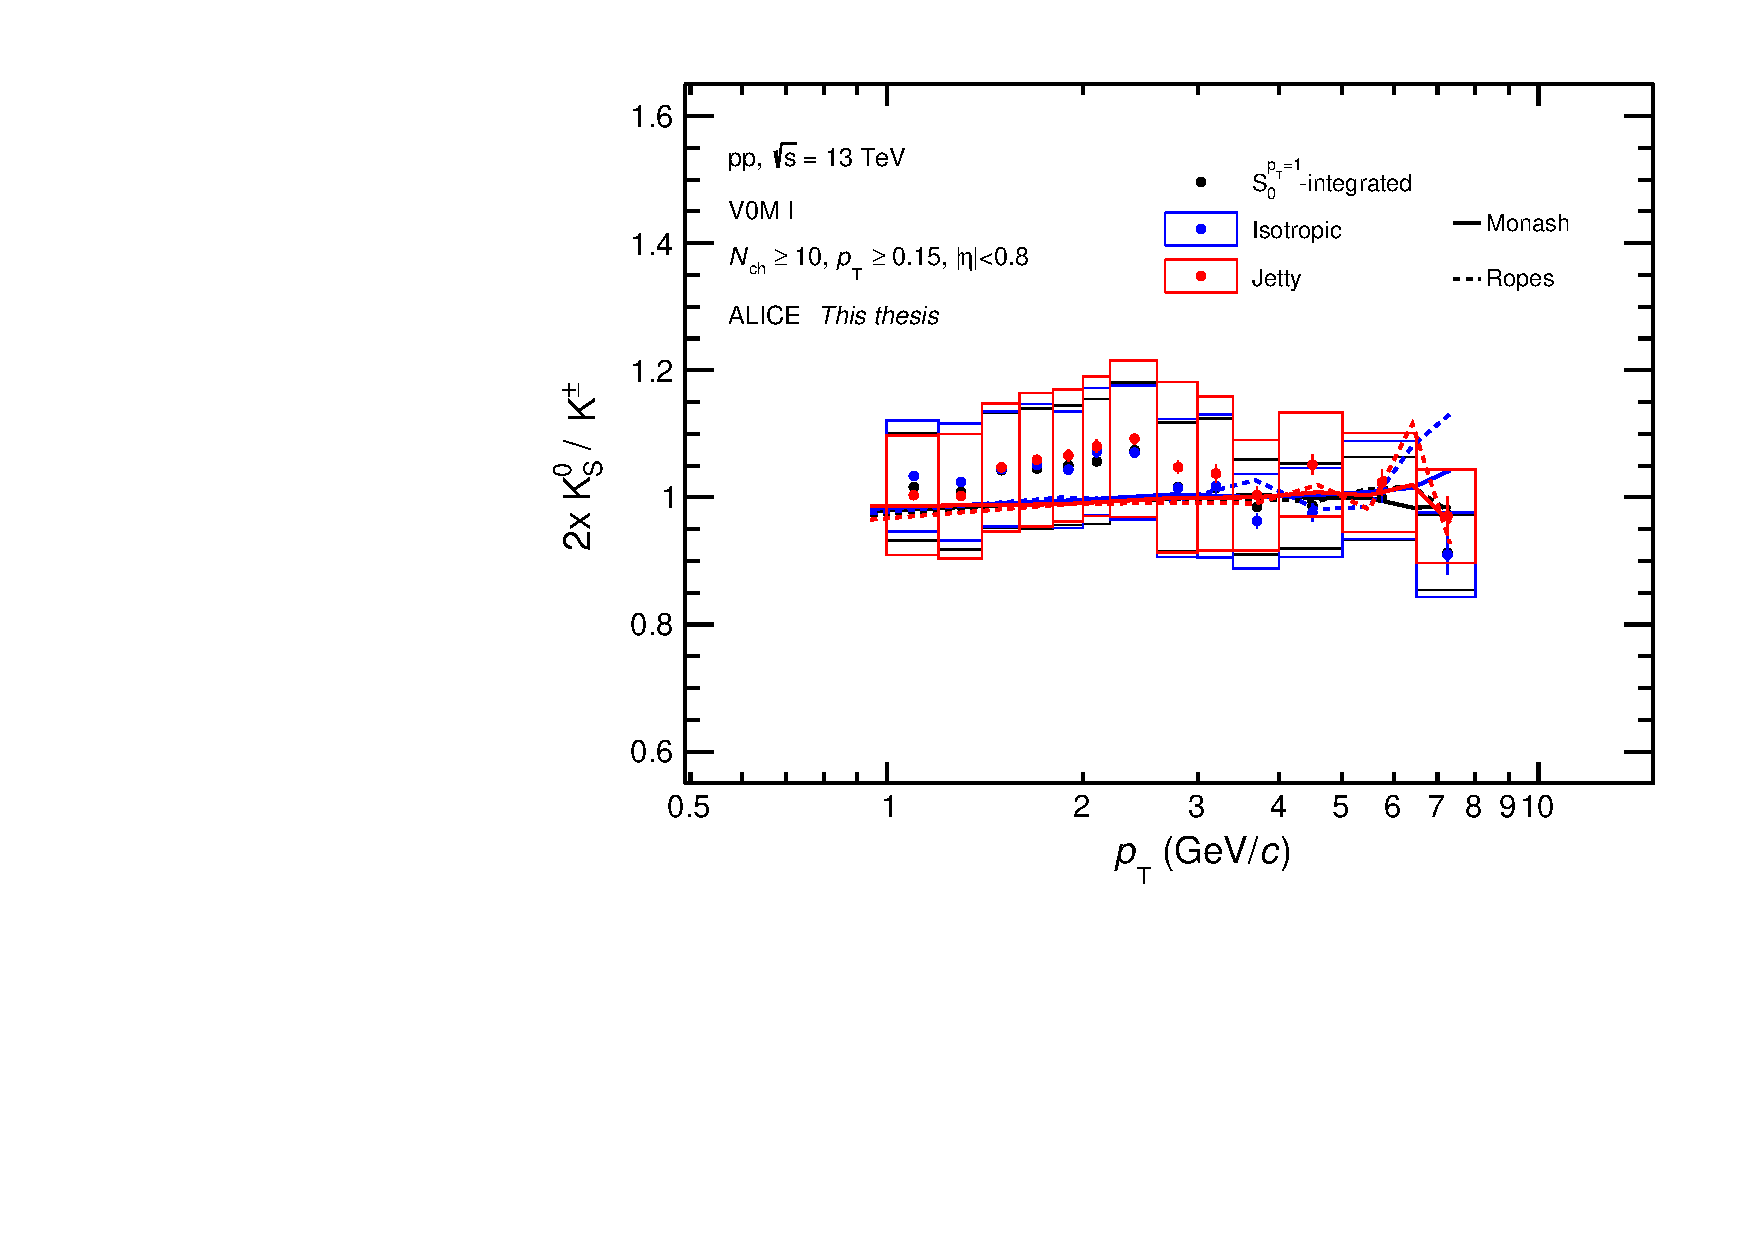
\includegraphics[width=.4\textwidth]{\imgpath/KtoK_V0M01_spher10.pdf}}
\caption{Ratios of transverse momentum spectra of \KOs to \kpm in \textbf{(a)} \NSPD I and \textbf{(b)} \VOM I high-multiplicity events, also showing the effect of spherocity selection. The results are compared with MC predictions of Pythia 8 tunes.}
\label{fig:sphero:ktok}
\end{figure}

\section{Mean transverse momenta and integrated yields}

The \meanpt and particle yields $\langle \dndy \rangle$ in different \SOPT bins for the \NSPD I class are reported in Fig.~\ref{fig:sphero:meanpt}. The measured values of \meanpt quantify the observations in the spectra: there is a significant \pt-hardening in jet-like events, consistently seen in both \KOs and \LA. Furthermore, the \meanpt of the inclusive high-multiplicity events is consistent with that of the isotropic subsample. This result suggests that the average high-multiplicity events and \SOPT-selected isotropic events are dominated by similar underlying physics processes.

Furthermore, the \SOPT-integrated event class is not simply the arithmetic average of the jetty and isotropic subsamples. This implies that jetty events are rare outliers of a much more homogeneous group of high-multiplicity events, which will be further focused on in the next sections.

\begin{figure}[H]
\subfloat[][]{\adjincludegraphics[trim={0 0 0 0},clip,height=10em]{\imgpath/meanpt.pdf}}\\
\subfloat[][]{\adjincludegraphics[trim={0 0 0 0},clip,height=10em]{\imgpath/meanpttopi.pdf}}\\
\subfloat[][]{\adjincludegraphics[trim={0 0 0 0},clip,height=10em]{\imgpath/dndy.pdf}}\\
\subfloat[][]{\adjincludegraphics[trim={0 0 0 0},clip,height=10em]{\imgpath/dndytopi.pdf}} 
\caption{\textbf{(a)} Mean transverse momentum and \textbf{(c)} integrated yields of \pip+\pim, \KOs, and \LA+\AL in jetty, isotropic, and \SOPT-unbiased high-multiplicity events determined at mid-rapidity. \textbf{(b,d)} Their ratios of \KOs and \LA+\AL to pions. \textit{CROP TO SHOW ONLY pi, \KOs, \LA.}}
\label{fig:sphero:meanpt}
\end{figure}

The results indicate that not only charged pions but also neutral \KOs and \LA show little variation in multiplicity between the different \SOPT extremes in the \NSPD I class, although more so for the latter two. This could be because of their smaller correlation with \SOPT as they are neutral, or it may suggest strangeness enhancement. The models generally provide good agreement with the measured \meanpt of \KOs, while the results for \LA are best described by the Pythia Ropes model. The yields for \KOs are also largely consistent with the models presented, whereas the Pythia Monash model does not match the \LA yields.

\section{Ratios to pions}

Rather than focusing on the models' inability to match the absolute values, this measurement can provide an opportunity to study the underlying dynamics that affect the heavier and stranger particles. To achieve this, the \KOs and \LA+\AL \pt spectra are divided by the \pip+\pim spectra. The results are presented in Fig.~\ref{fig:sphero:ktopi} and Fig.~\ref{fig:sphero:ltopi}.

The data reveals overall suppression of \KOs in jetty events and enhancement in isotropic events in the measured \pt range. The effect is observed, although in different ways, in all three event classes: \NSPD I (where spherocity is assumed to change mostly the \meanpt), \NSPD I-III (where spherocity is assumed to change both the \meanpt and multiplicity), and \VOM I (where spherocity is assumed to change mostly the multiplicity). The \LA ratios behave similarly but an enhancement in low-\pt is observed in the \VOM I case, resembling typical radial flow signatures.

The presented models cannot describe the ratios to pions, although the trends relative to the \SOPT-unbiased case are reproduced well.

\begin{figure}[H]%
\centering%
\subfloat[][]{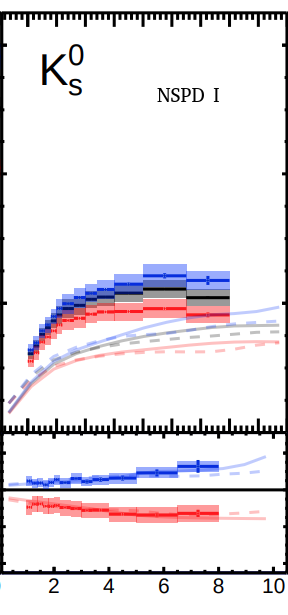
\includegraphics[width=.25\textwidth]{\imgpath/ktopi_nch01.png}}\hspace{1em}
\subfloat[][]{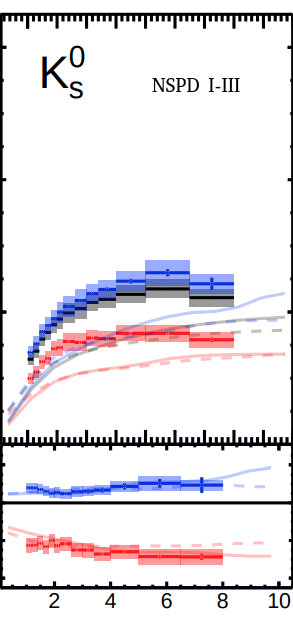
\includegraphics[width=.25\textwidth]{\imgpath/ktopi_nch.png}}\hspace{1em}
\subfloat[][]{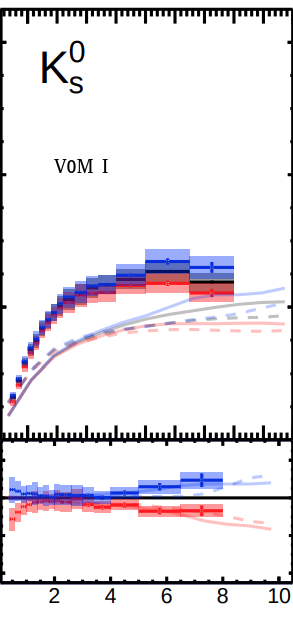
\includegraphics[width=.25\textwidth]{\imgpath/ktopi_v0m01.png}}
\caption{Ratios of transverse momentum spectra of \KOs to \pip+\pim in jetty, isotropic, and \SOPT-unbiased in events with high-multiplicity classes \textbf{(a)} \NSPD I, \textbf{(b)} \NSPD I-III, and \textbf{(c)} \VOM I. Statistical and systematic uncertainties are depicted as error bars and boxes, respectively.}
\label{fig:sphero:ktopi}
\end{figure}

\begin{figure}[H]%
\centering%
\subfloat[][]{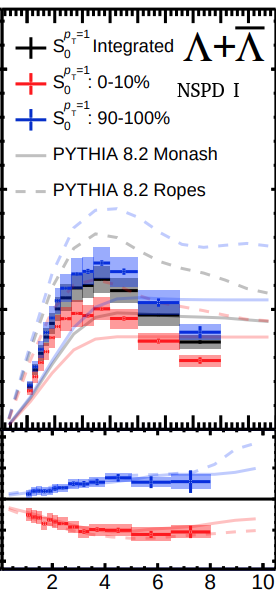
\includegraphics[width=.25\textwidth]{\imgpath/ltopi_nch01.png}}\hspace{1em}
\subfloat[][]{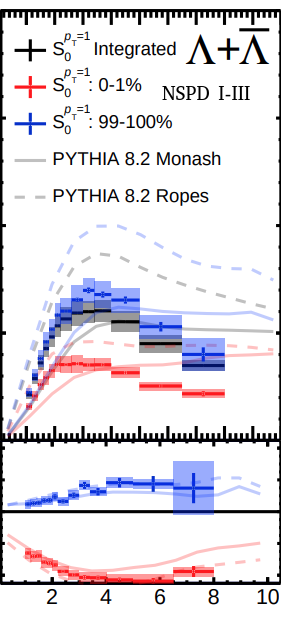
\includegraphics[width=.25\textwidth]{\imgpath/ltopi_nch.png}}\hspace{1em}
\subfloat[][]{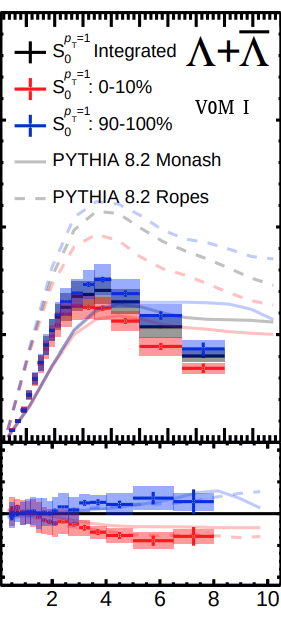
\includegraphics[width=.25\textwidth]{\imgpath/ltopi_v0m01.png}}
\caption{Ratios of transverse momentum spectra of \LA+\AL to \pip+\pim in jetty, isotropic, and \SOPT-unbiased in events with high-multiplicity classes \textbf{(a)} \NSPD I, \textbf{(b)} \NSPD I-III, and \textbf{(c)} \VOM I. Statistical and systematic uncertainties are depicted as error bars and boxes, respectively.}
\label{fig:sphero:ltopi}
\end{figure}

\section{Baryon-to-meson ratio}

The baryon-to-meson ratio \ltok was investigated in this study, as it is a common observable used to measure the effects of radial flow, as discussed in Section X. To focus on the different functions of \SOPT selection in the different high-multiplicity classes, the results for the \NSPD I and \VOM I events are shown in Fig.~\ref{fig:sphero:ltok}. They are also juxtaposed with the \ptopi ratios \cite{vazquezruedaStudyProductionPp2022}. The ratios reveal a significant increase when transitioning from jetty to isotropic events, indicating that the production of heavier $\LA$ is systematically more suppressed in jetty events than \KOs. Similar observations have been made in other ALICE measurements studying jets (discussed further in \ref{sec:rt:btom}) \cite{acharyaProductionKS0Jets2022}.

Although the increase in the ratio is consistent with the typical signatures of radial flow, the \NSPD I results do not reveal the depletion at low \pt and neither results show the shift of the peak to higher \pt, both of which are also its characteristic features. Additionally, the data are compared with the two tunes of Pythia 8, favouring the Ropes configuration.

\begin{figure}[H]
%\subfloat[][]{\adjincludegraphics[trim={0 0 {0.32\width} 0},clip,height=15em]{\imgpath/ratiosBaryonMeson.pdf}}\\
\subfloat[][]{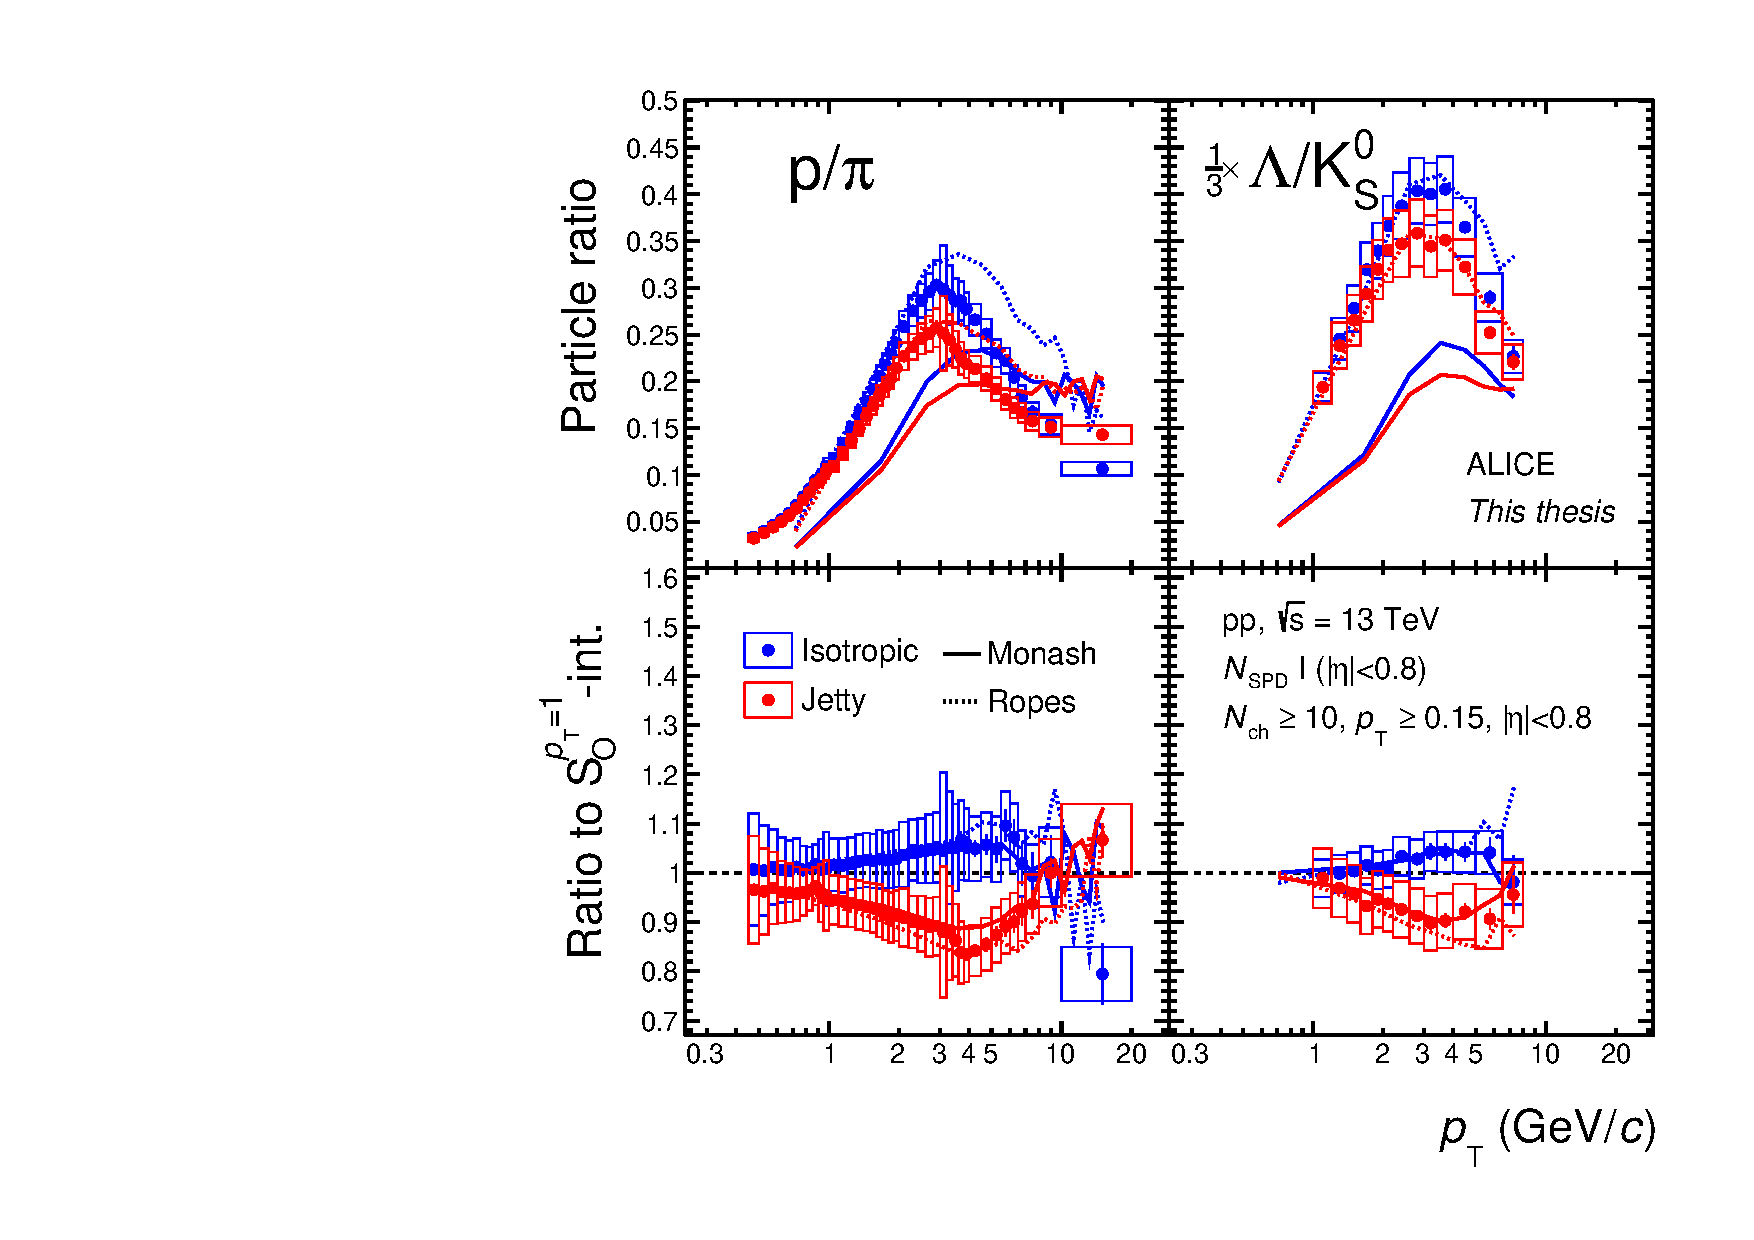
\includegraphics[width=.49\textwidth]{\imgpath/ratiosBaryonMesonNCharged01.pdf}}
\subfloat[][]{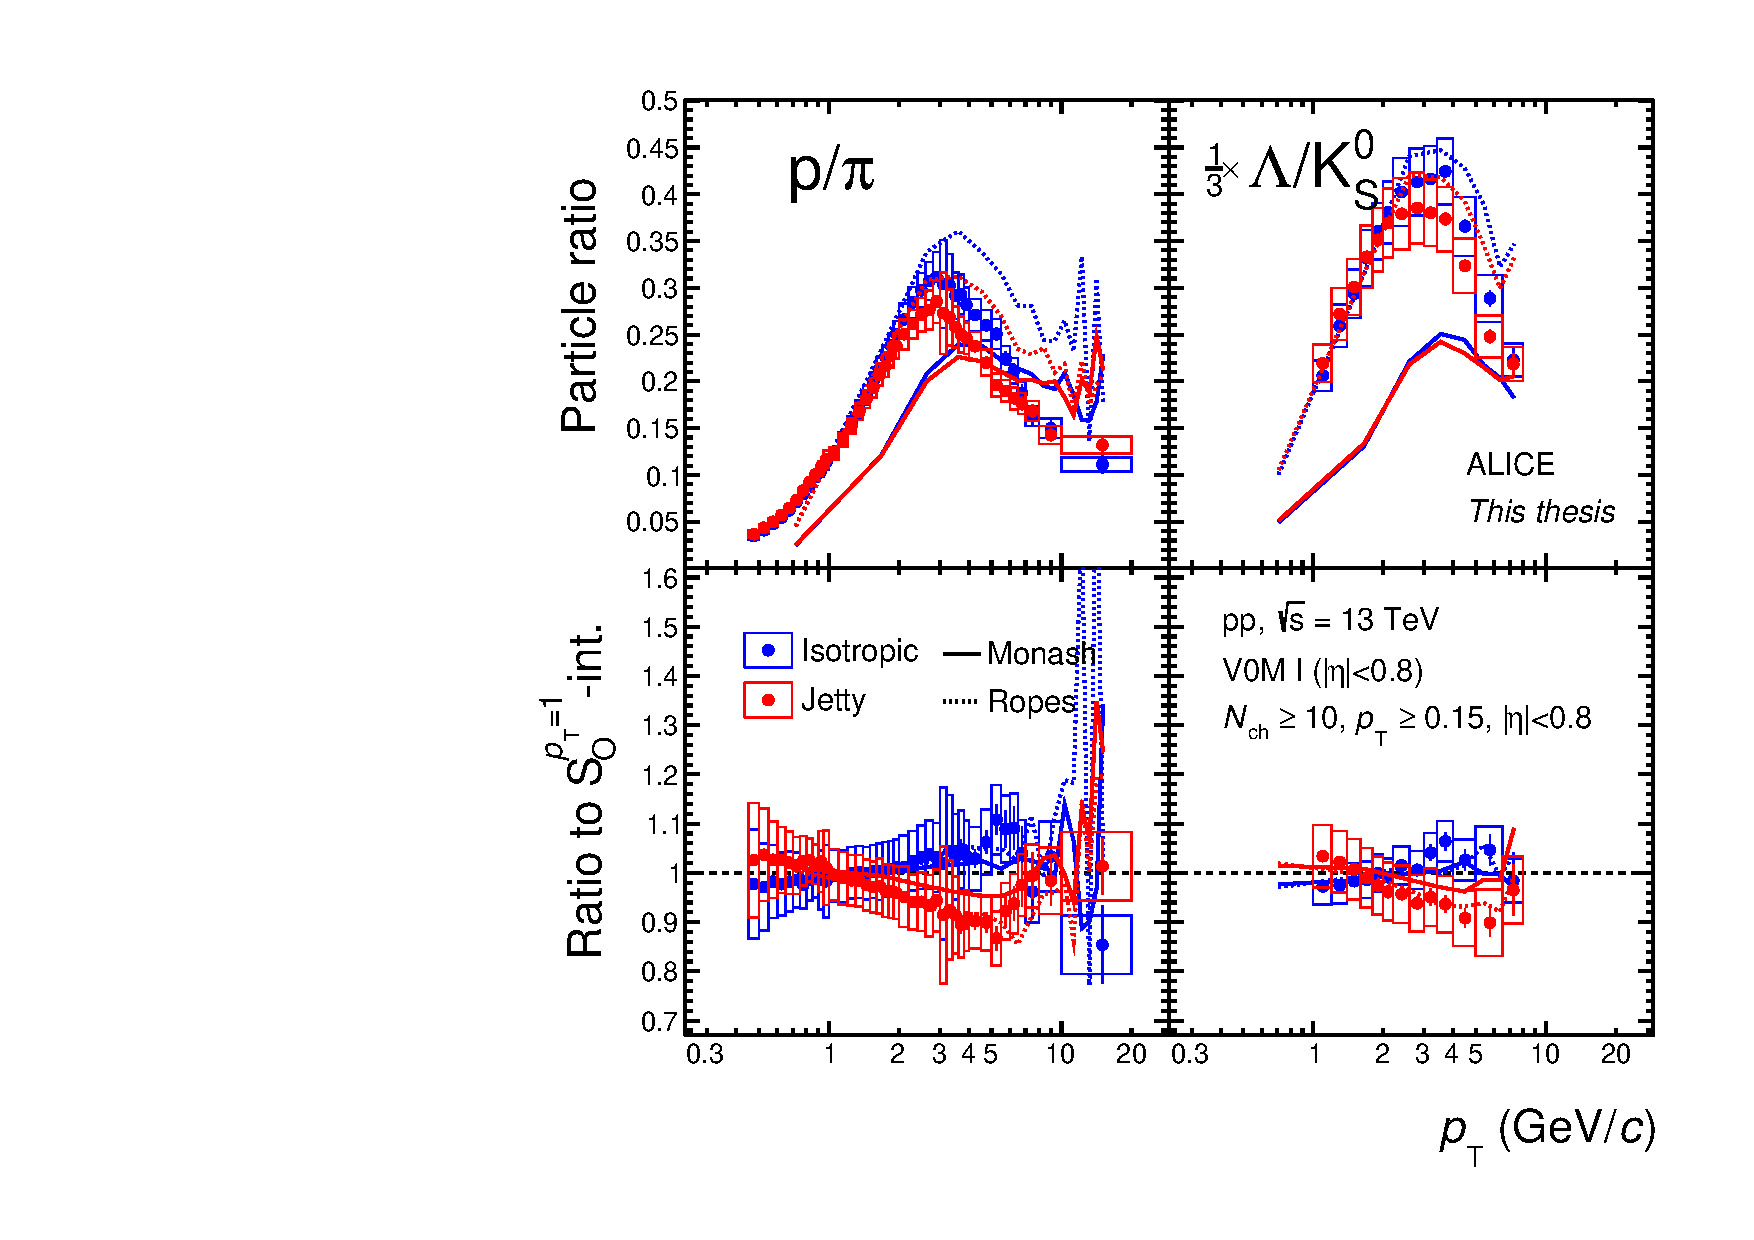
\includegraphics[width=.49\textwidth]{\imgpath/ratiosBaryonMesonV0M01.pdf}}
\caption{Baryon-to-meson ratios of the jetty ($0-10\%$) and isotropic ($90-100\%$) transverse momentum spectra of p to $\pi$ and \LA+\AL to \KOs in the \textbf{(a)} \NSPD I and \textbf{(b)} \VOM I high-multiplicity events of pp collisions at \sppt{13}. The bottom panels display the ratios to the \SOPT-unbiased case. MC predictions are denoted as lines, statistical uncertainties as error bars, and systematic uncertainties as error boxes.}
\label{fig:sphero:ltok}
\end{figure}

\section{Ratio of integrated yields vs. \SOPT}

The main contribution of this study is the investigation of strangeness production as a function of \SOPT. Yields of the \LA baryon were determined in \NSPD I and \VOM I classes in the following intervals of \SOPT: $0-1\%$, $1-5\%$, $5-10\%$, $10-20\%$, $20-80\%$, $80-90\%$, $90-95\%$, $95-99\%$, and $99-100\%$. The integration was done in the measured \pt range rather than extrapolated. The \SOPT-dependent \LA yields are then divided by \SOPT-dependent pion yields as a reference. The effects of not extrapolating were studied and found to be unimportant, and while the extrapolation confirms the physics message of the default method, it also increases systematic uncertainties. 

The results, together also with p ($|S|=0$) and \XI ($|S|=2$) are reported in Fig.~\ref{fig:sphero:lvssOpt}. For the \NSPD I events, there is a clear strangeness- and/or mass-dependent enhancement with increasing \SOPT. It is important to emphasize that in this event class, the \Nch multiplicity is basically fixed. Therefore, these effects are results of the different underlying dynamics of the collisions, specifically the varying hardness of involved scatterings, rather than merely an effect of increased \Nch.

Conversely, the \VOM I events show no such dependence, and jetty and isotropic events appear to produce the same relative amount of strangeness. This goes against intuition that varying \Nch between jetty ($\Nch \to 15$) and isotropic events ($\Nch \to 30$, according to Fig.~\ref{fig:sphero:v0mvscl1}) should introduce an effect, in accordance with traditional studies of strangeness enhancement in pp collisions as a function of \Nch. This observation is not fully understood, but it suggests that the decrease in strangeness in jetty events due to the decrease in \Nch and  increase in \meanpt is not trivial and counterbalanced by some other factors of the collision.

Finally, the results were compared with MC predictions, and only Pythia 8 Ropes accurately captures the observed trends and, to some extent, the magnitudes.

\begin{figure}[H]
\centering%
\subfloat[][]{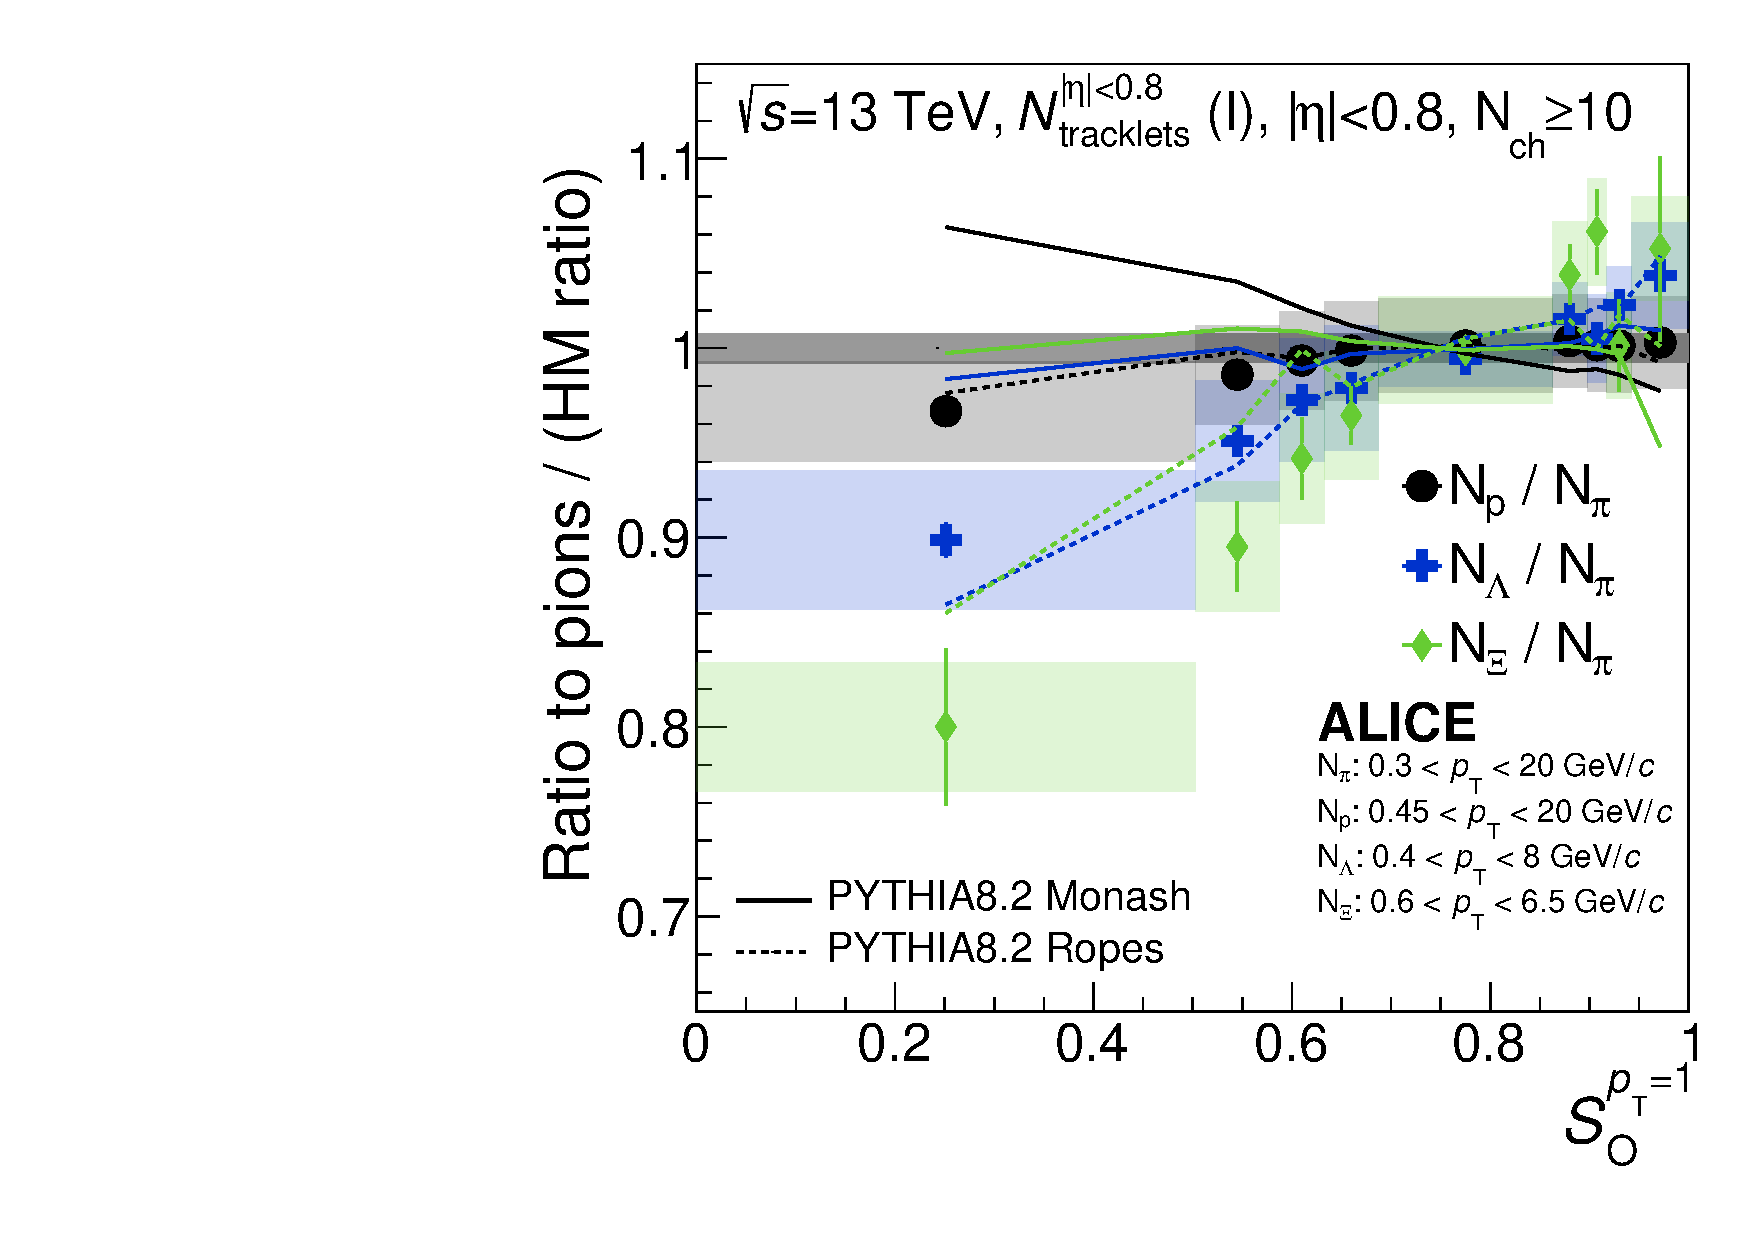
\includegraphics[width=.45\textwidth]{\imgpath/xi_over_pi_vs_So_CL1_01_PY.pdf}}
\subfloat[][]{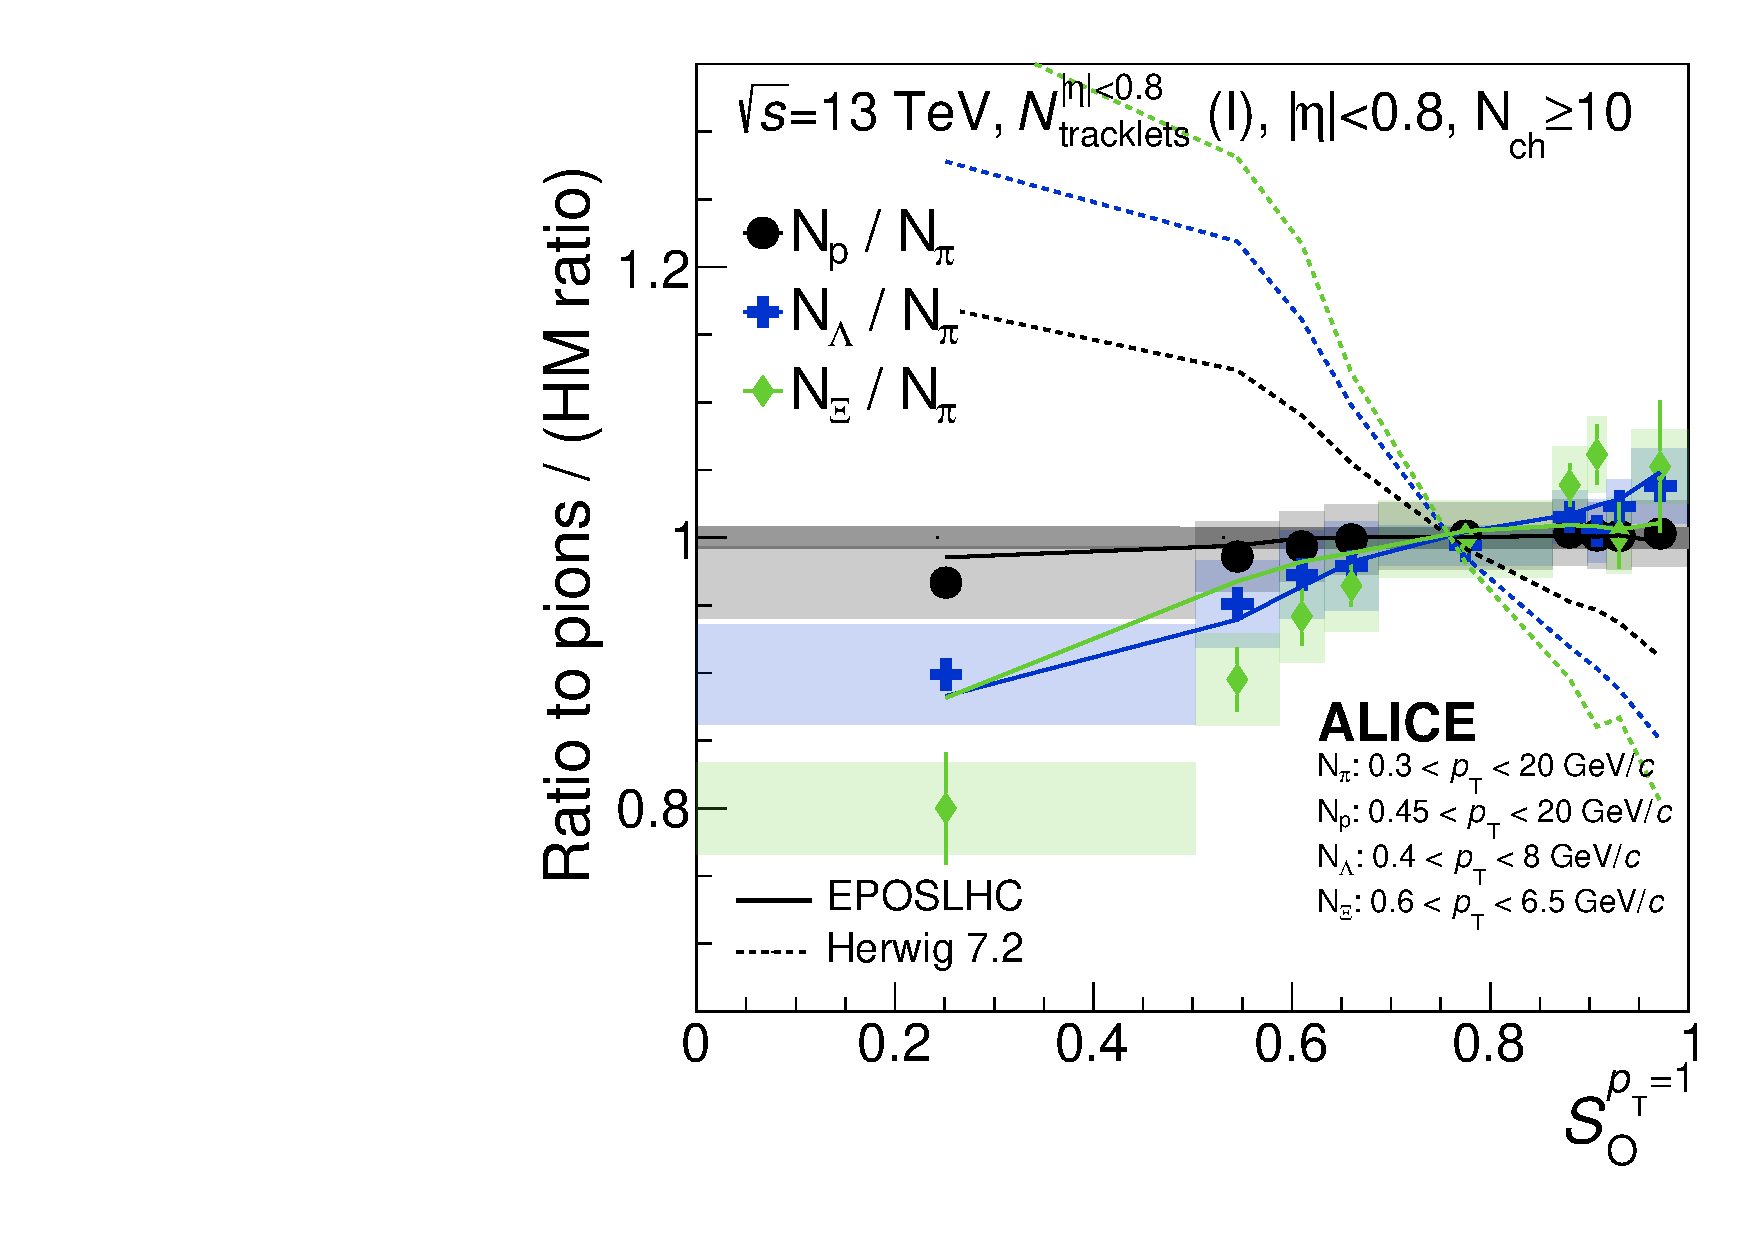
\includegraphics[width=.45\textwidth]{\imgpath/xi_over_pi_vs_So_CL1_01_HW.pdf}}\\
\subfloat[][]{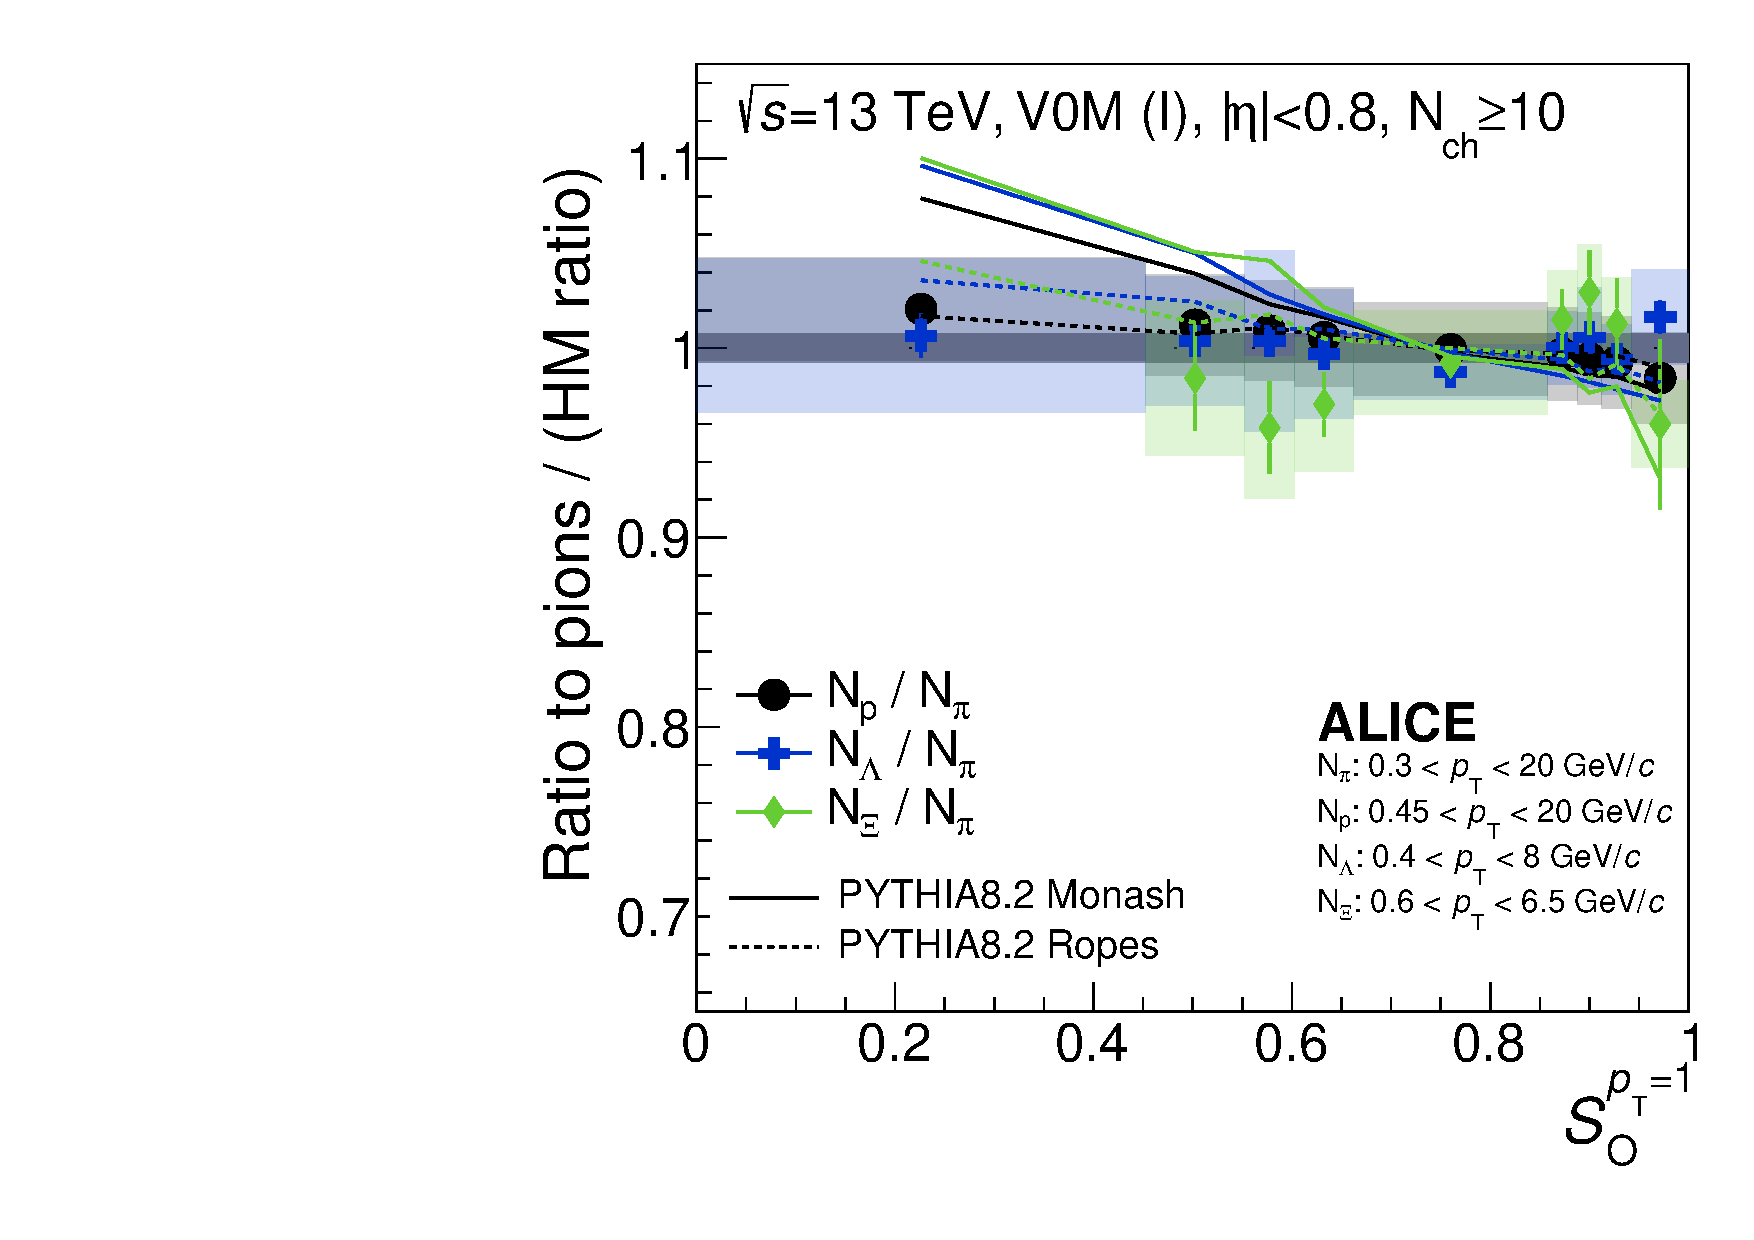
\includegraphics[width=.45\textwidth]{\imgpath/xi_over_pi_vs_So_V0M_01_PY.pdf}}
\subfloat[][]{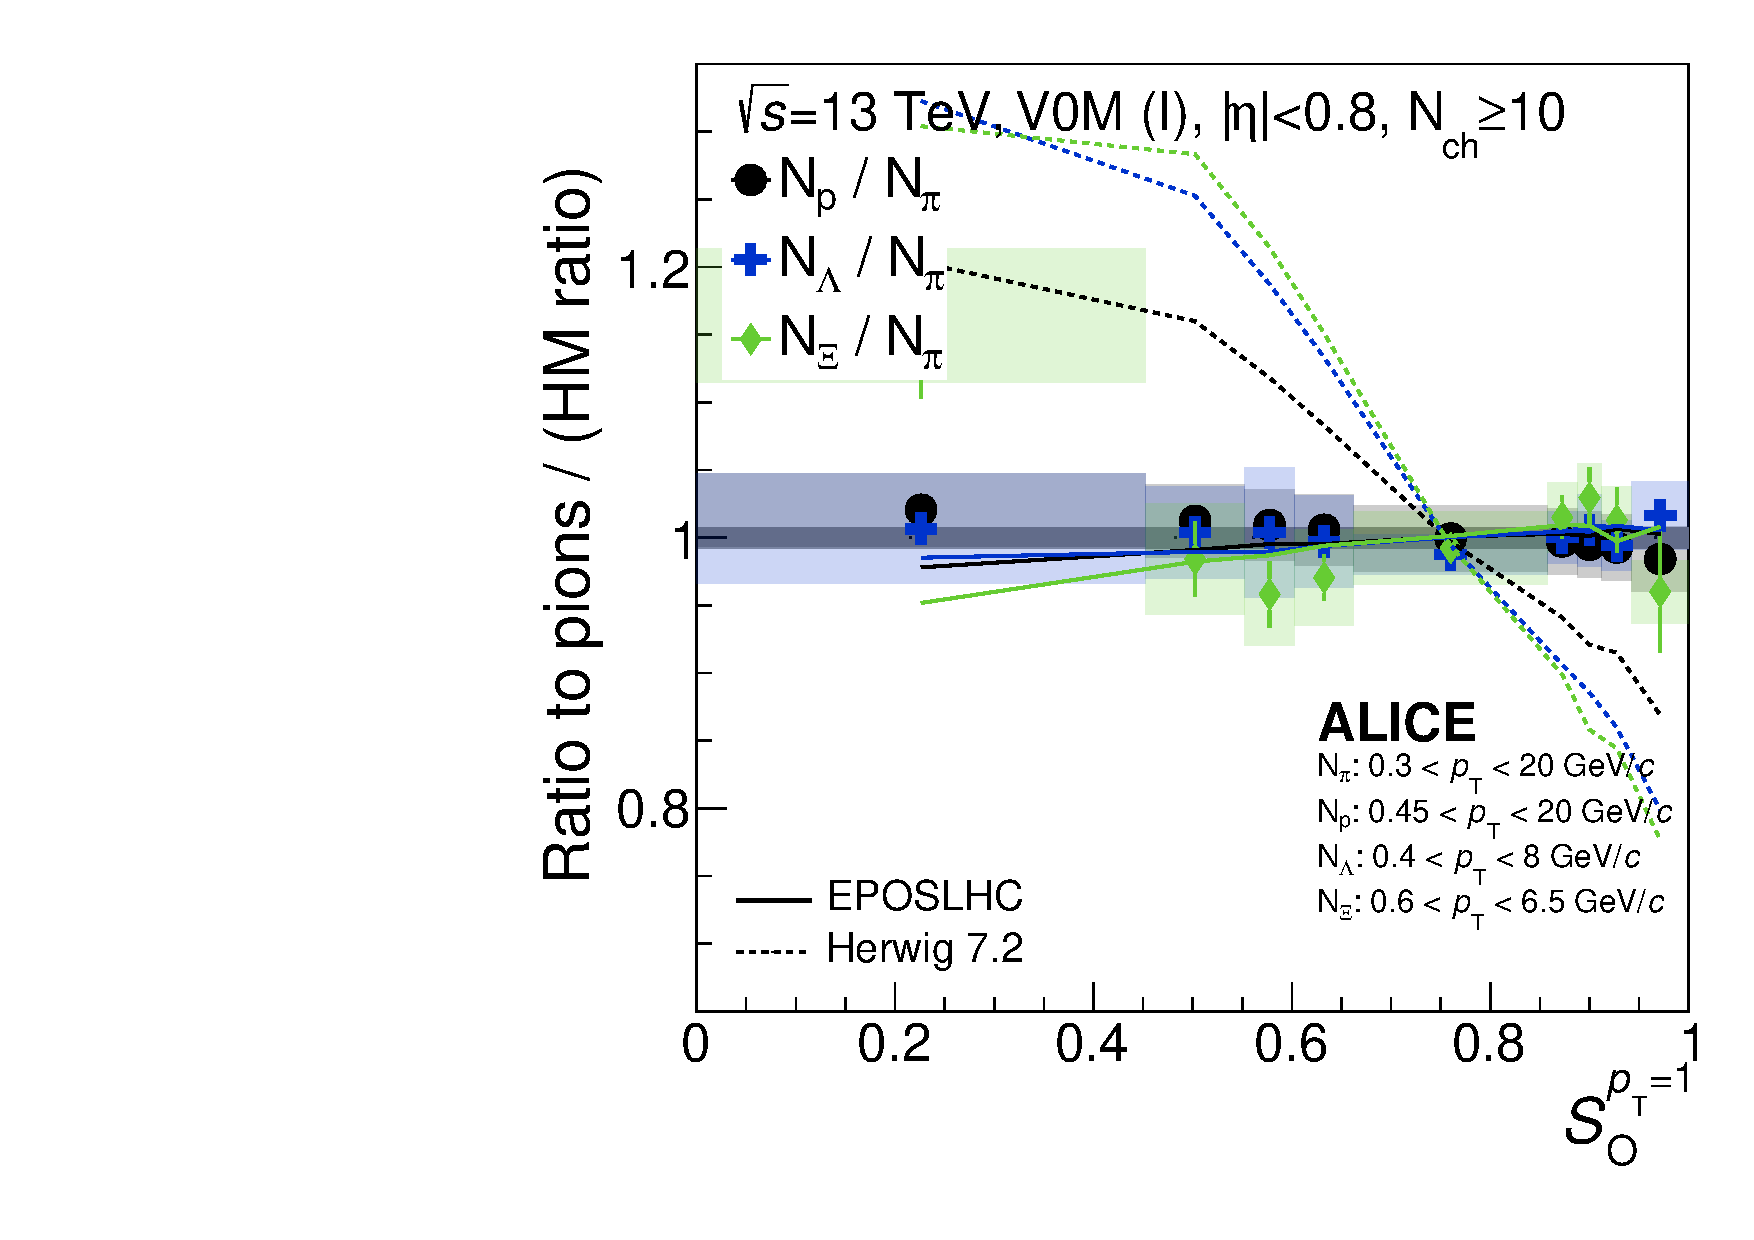
\includegraphics[width=.45\textwidth]{\imgpath/xi_over_pi_vs_So_V0M_01_HW.pdf}}\\
\caption{Double-ratios of integrated yields with respect to pions as a function of \SOPT in the \NSPD I and \VOM I events. Statistical and total systematic uncertainties are shown by bars and boxes, respectively. The curves represent different model predictions of the same measurement: \textbf{(a)},\textbf{(c)} Pythia Monash and Ropes, \textbf{(b)},\textbf{(d)} EPOS LHC and Herwig.}
\label{fig:sphero:lvssOpt}
\end{figure}
